\documentclass[10pt]{article}

\usepackage{blindtext}
\usepackage{etex}
\usepackage{makeidx}  % allows for indexgeneration
\usepackage{mathtools} %
\usepackage{booktabs} %
\usepackage{verbatim} %
\usepackage{graphicx} 
\usepackage{amsmath}
\usepackage{amssymb}
\usepackage{amsthm}
\usepackage{xspace}
\usepackage{natbib}
\usepackage{pifont}%
\usepackage{tikz}
\usepackage{relsize}
\usepackage{multirow}
\usepackage{textcomp}
\usepackage{comment}
\usepackage{url}
\usepackage{float}
\usepackage{algorithm}
\usepackage{algpseudocode}
\usepackage{subfig}
\usepackage{framed}
\usepackage{empheq}

\newcommand{\cmark}{\ding{51}}%
\newcommand{\xmark}{\ding{55}}%
\newcommand{\vectornorm}[1]{\left|\left|#1\right|\right|}
\newcommand{\argmin}{\operatornamewithlimits{argmin}}
\newcommand{\argmax}{\operatornamewithlimits{argmax}}

\algdef{SE}[DOWHILE]{Do}{doWhile}{\algorithmicdo}[1]{\algorithmicwhile\ #1}%

\newtheorem{problem}{Problem}

\newcommand{\Tempselect}{\textit{TempSelect}\xspace}

\excludecomment{plots}
%\includecomment{plots}

\begin{document}

\title{Efficient Selection of Optimal Time Points Over Biological Time-Series Data}
\date{}

\maketitle

\section{Methods}

\subsection{Problem statement}
Our goal is to identify a (small) subset of time points that can be
used to accurately reconstruct the expression trajectory for {\em
all} genes or other molecules being profiled. We assume that we can
efficiently and cheaply obtain a dense sample for the expression of
a very small subset of representative genes (here we use nanostring
to profile less than $0.5\%$ of all genes) and attempt to use this
subset to determine optimal sampling points for the entire set of
genes.

Formally, let $G$ be the set of genes we have profiled in our dense
sample, $T = \{t_{1}, t_{2}, \ldots, t_{T}\}$ be the set of all
sampled time points. We assume that for each time point we have $R$
repeats for all genes. We denote by $e_{gt}^{r}$ be the expression
value for gene $g \in G$ at time $t \in T$ in the $r$'th repeat for
that time point. We define $D_{g} = \{e_{gt}^{r}\,,\, t \in T, r \in
R$ as the complete data for gene $g$ over all replicates and time
points $T$.

To constrain the set of points we select we assume that we have a
predefined budget $k$ for the maximum number of time points we can
sample in the complete experiment (i.e. for profiling all genes, miRNAs, epigenetic marks etc. using high throughput seq
experiments). We are interested in selecting $k$ time points from
$T$ which, when using only the data collected at these $k$ points,
minimizes the prediction error for the expression values of the
unused points. To evaluate such a selection, we use the selected
values to obtain a smoothing spline~\cite{deboor, bar2003,
wahba1990} function for each gene and compare the predicted values
based on the spline to the measured value for the non-selected
points to determine the error. In our problem, $t_{1}$ and $t_{T}$
define the first and end points, so they are always selected. The
rest of the points are selected to maximize the following
objective~\ref{prob:prob1}:
%
\begin{problem}\label{prob:prob1}
Given $D_{g}$ for genes $g \in G$, the number of desired time points
$k$, identify a subset of $k-2$ time points in $T \setminus \{t_{1},
t_{T}\}$ which minimizes the prediction error for the expression
values of all genes in the remaining time points.
\end{problem}


\subsection{Spline assignments}

Before discussing the actual procedure we use to select the set of
time points, we discuss the method we use to assign splines based on
a selected subset of points for each gene. There are two issues
that needs to be resolved when assigning such smoothing splines: 1.
The number of knots (control points) and 2. their spacing. Past
approaches for using splines to model time series gene expression
data have usually used the same number of control points for all
genes regardless of their trajectories~\cite{bar2012, singh2005}, and mostly employed uniform
knot placements. However, since our method needs to be able to adapt
to any size of $k$ as defined above, we select them indirectly through
regularization parameter of the fitted cubic smoothing spline where number
of knots will be increased until the smoothing condition is
satisfied~\cite{wahba1990}. Regularization parameter is estimated by leave-one-out cross-validation~(LOOCV).
%Given number of knots, it simply starts by uniform knot
%placement and iteratively improves it in a data-adaptive fashion. It repeats this procedure
%multiple times and returns the best solution. 

\subsection{\Tempselect: Iterative process to select points}\label{sec:mainalgo}

%We also emply a combinatorial procedure when number of points is less than.
Because of the highly combinatorial nature of the time points, selection problem we rely on a greedy iterative process to select
the optimal points as shown in Algorithm~\ref{alg:algo}.

There are three key steps in this algorithm which we discuss in
detail below.

\begin{itemize}
\item {\em Selecting the initial set of points:} When using an iterative algorithm to solve non-convex problems with several local minima,
a key issue is the appropriate selection of the initial solution set~\cite{kmeans, mixture}. We have tested a number
of methods for performing such initializations. The simplest method
we tried is to uniformly select a subset of the points (so if
$k=T/4$ we use each 4'th point). Another method we tested is to partition the set
of all time points $T$ into $k-1$ intervals of almost equal size. This
method determines these boundaries by estimating the cumulative number of points until each time point and
selecting time points with cumulative values $\frac{T}{k-1}, 2\frac{T}{k-1},
\ldots, (k-2)\frac{T}{k-1}$ respectively. Then, it uses $k$ interval
boundaries including $t_{1}$ and $t_{T}$ as initial solution. Finally, we tested a
method that relies on the changes between consecutive time points to
select the most important ones for our initial set. Specifically, we sort all points except $t_{1}$ and $t_{T}$ by average
absolute difference with respect to its predecessor and successor time points by
computing:
%
\begin{equation}
m_{t_{i}} = \frac{\sum_{g \in G}\,|Md(e_{g t_{i-1}}) - Md(e_{g t_{i}})| + |Md(e_{g t_{i+1}}) - Md(e_{g t_{i}})|}{2|G|}
\end{equation}
%
where $Md(e_{g t_{i}})$ is the median expression for gene $g$ at
time $t_{i}$. We then select the $k-2$ points with maximum $m_{t_{i}}$
as the initial solution.

\item {\em Iterative improvement step:} After selecting the initial set, we begin the iterative process of refining the subset of selected points.
In this step we repeat the following analysis in each iteration. We
exhaustively remove all points from the existing solution (one at a
time) and replace it with all points that were not in the selected
set (again, one at a time). For each pair of such point, we compute
the error resulting from the change (using the splines computed
based on the current set of points evaluated on the left out time
points), and determine if the new point reduces the error or not.
Formally, let $T^{-} = T \setminus \{t_{1}, t_{T}\}$ and $C_n$ be set of points for iteration $n$. We are
interested in finding a point pair $(t_{a} \in C_n, t_{b} \in T^{-}
\setminus C_n)$ which minimizes the following error ratio for the next iteration $C_{n+} =
C_n \setminus \{t_{a}\} \cup \{t_{b}\}$:
%
\begin{equation}
\textit{error ratio} = \frac{error(C_{n+})}{error(C_{n})} = \frac{\sum_{g \in G} \sum_{r \in R}\, \sum_{t \in
    T \setminus C_{n+}} (\hat{e}_{gt}^{C_{n+}} - e_{gt}^{r})^{2}}{\sum_{g \in G}
  \sum_{r \in R} \sum_{t \in
    T \setminus C_{n}} (\hat{e}_{gt}^{C_{n}} - e_{gt}^{r})^{2}}
\end{equation}
%
where $\hat{e}_{gt}^{C_{n}}$ is our spline based estimate of the expression
of gene $g$ at time $t$ by fitting smoothing spline over points
$C_{n}$. If there are pairs which leads to an error ratio
of less than $1$ in the above function, we select the best (lowest
error), assign it to $C_{n+1}$ and continue the iterative process. Otherwise we terminate
the process and output $C_n$ as the optimal solution. Note that this
greedy process is guaranteed to converge to a (local) minima since
the number of time points is finite.

% \begin{figure}
% \centering
% 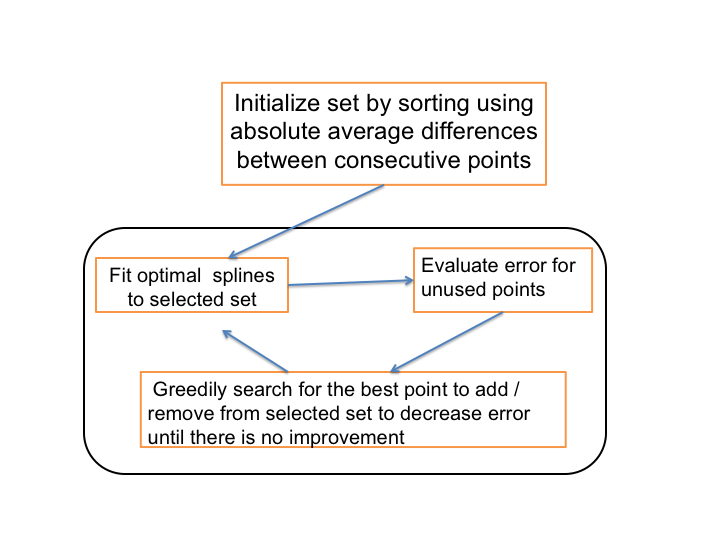
\includegraphics[scale=0.4]{algo.png}
% \caption{Summary of our Method}
% \label{fig:algo}
% \end{figure}

\begin{algorithm}
\caption{\Tempselect: Iterative $k$-point selection}
\label{alg:algo}
\begin{algorithmic}[1]
\Procedure{Iterative\textendash Temporal\textendash Selection}{}
\State $C_{0} = $ select initial $k$ time points by absolute difference sorting
\State $e_{0} = $ error of remaining points by fitting splines to $C_{0}$
\State $i=0$
\Do 
\For{each pair $(t_{a}, t_{b}) \in (T^{-} \setminus C_{i}) \times C_{i}$}
\State $C^{*} = C_{i} \cup \{ t_{a} \} \setminus \{ t_{b}\}$ 
\State $e^{*} = $ estimate error by fitting smoothing spline to
$C^{*}$ where \par 
\hspace{1.62cm} regularization parameter is estimated by LOOCV
\If{$e^{*} < e_{i}$}
\State $C_{i+1} = C^{*}$ 
\State $e_{i+1} = e^{*}$
\EndIf
\State $i = i+1$
\EndFor
\doWhile{$e_{i+1} < e_{i}$}
\State Output $C_{i}$ and $e_{i}$
\EndProcedure
\end{algorithmic}
\end{algorithm}

\item {\em Fitting smoothing spline:} Third key step of our approach
  is fitting smoothing spline to every gene independently for selected
  subset of time points. Smoothing splines are capable of modeling
  arbitrary nonlinear shapes as well as they do not have the problems seen in other polynomial fitting
  methods such as Runge's phenomenon. Smoothing splines perform quite well in preventing overfitting~\cite{wahba1990}. Let
  $I_{g} = \{(t, Md(e_{gt})),\, t \in C \}$, and $\mu$ be the spline we are interested in fitting, smoothing spline
  can be found by the following optimization problem which minimizes
  penalized least-squares error:
%
\begin{equation}
\min \sum_{(t, y_{t}) \in I_{g}} \,(y_{t} - \mu(t))^{2} + \lambda
\int_{t_{1}}^{t_{T}} \mu^{''}(x)^{2} dx
\end{equation}
%
where $\lambda$ is the regularization parameter which prevents
overfitting by affecting the number of knots selected. We estimated regularization parameter by
leave-one-out cross-validation (LOOCV) in our experiments.

\end{itemize}


\subsection{Individual vs. Cluster based Evaluation}\label{sec:clusteval}

In section~\ref{sec:mainalgo}, we assume that error of each gene has
same contribution to the overall error. However, this assumption
ignores the fact that expression profiles of genes are correlated with the expression of other genes. To take the
correlation between gene profiles into account, we also performed cluster
based evaluation of genes where we analyzed the error by weighting each gene in terms of inverse of the numbers of
genes in the cluster it belongs. This scheme ensures that each cluster
contributes equally to the resulting error rather than each gene. We
find clusters by k-means algorithm over time series-data by treating each gene as a
point in $R^{T}$ space as well as over a vector of
randomly sampled $T$ time points on fitted spline~\cite{bishop2006}. We use Bayesian Information Criterion~(BIC) to
determine the optimal number of clusters~\cite{bic}.

\subsection{More Complex Iterative Improvement Procedures}\label{sec:complexiter}

We also propose the following more complex iterative improvement procedures for \Tempselect:

\begin{itemize}
\item We add and remove $b$ time points in each iteration instead of a single point. This increases the complexity of each
  iteration from $O(kGT^{2}Q)$ to $O(kGT^{2b}Q)$ where $Q$ is
  the complexity of fitting a smoothing spline.

\item We run simulated annealing to escape from local
  minima~\cite{kirkpatrick1983}. In this case, we do not always move
  to a pair of points with the minimum error in each iteration, but
  instead move to a solution with random pair of points with probability $1$ if
  its error $e^{r}$ is lower than error of current solution $e^{i}$ whereas we move to a solution with probability
  $e^{-T(e^{r}-e^{i})}$ if $e^{r} \ge e^{i}$. Here, $T$ is the temperature that increases by
  increasing number of iterations and the probability of moving to a solution
  with larger error decreases over time.
\end{itemize}

Even though both approaches should escape from local minima theoretically better than
the greedy approach we described above, they do not perform significantly
better in practical instances.

\section{Results}

\subsection{Datasets and Implementation}

We developed a method \Tempselect to select a subset of $k$ time points from an
initial larger set of $n$ points such that the selected subset provides an accurate, yet compact, representation of the temporal
trajectory. The method utilizes splines to represent temporal profiles and implements a cross
validation strategy to evaluate potential sets of points. Following
initialization which is based on the expression values, we employ a
greedy search procedure that adds and removes points until a local minima is reached. The resulting
set is then used for the larger genomic and epigenetic experiments. To test this method and to demonstrate its ability to reduce time,
costs and samples while still providing accurate description of the
temporal profiles, we focused on experiments related to lung
development in mice. We implemented \Tempselect in Python. Its implementation, code, detailed results, and datasets are available
on~\url{https://github.com/emresefer/geneexpress}. 

We have used mRNA and miRNA expression datasets as well as temporal histone
methylation dataset over Mus Musculus in our analysis. mRNA dataset is obtained by profiling the expression of $126$ selected
genes that are determined to be effective in lung development via NanoString array at a
high sampling rate. On the other hand, larger miRNA dataset
profiles the expression of $599$ microRNAs. Both mRNA and
miRNA datasets includes samples at $40$ time points between the half and
$28$'th days in mouse development. mRNA dataset has between $2$ and
$4$ repeats for each time point whereas miRNA dataset has between $3$
and $4$ repeats for each time point. We normalized mRNA dataset by
quantile normalization followed by $\log 2$ transformation whereas
miRNA values are normalized by variance mean normalization~\cite{bolstad2003}. Methylation data has $3$ repeats for time
points $0.5$, $1.5$, $2.5$, $5$, $10$, $15$, $19$, $26$ for $266$ loci
belonging to $13$ genes. Among these genes all of them except Zfp536 also exist in
mRNA dataset. Supplementary Table~\ref{tab:sup1} summarizes the number of loci for each gene in methylation
dataset. We used shifted percentage of methylation at each time
point as our dataset which is obtained by subtracting the median percentage of
methylation at initial time point~(baseline) from all data points for each gene.

\subsection{\Tempselect identifies subset of important time points across multiple genes}\label{sec:findsubset}

%identified points
While our method can be used to select any number of time points, to demonstrate its utility we have tested it
in the following setting. First we fixed a set of points in advance (first~($0.5$'th day) and
last~($28$'th day), which are required for any setting and day $7$ which was
previously determined to be of importance to lung development, see
Supplementary Results for other settings). In addition, we have asked
\Tempselect to further select $10$ more points (for a total of $13$). For
this setting, the method selected the following points: $0.5$,
$1.0$, $1.5$, $2.5$, $4$, $5$, $7$, $10$, $13.5$, $15$, $19$, $23$,
$28$ out of $40$ points. While we do not know the ground truth, the larger focus on the
earlier time points determined by the method (with $7$ of the $13$
points for the first $7$ days) makes sense in this context as several
aspects of lung differentiation are determined in this early phase~\cite{guilliams2013}. The other $3$ weeks were more or less
uniformly sampled by our method. This highlights the usefulness of
an unbiased approach to sampling time points rather than just
uniformly sampling through the time window.

%comparison
We tested the performance of our method by using it to select
subsets of size $3$ to $25$ time points. To determine the accuracy of the reconstructed profiles
using the selected points, we computed the average mean squared error for points
that were not used by the method (Methods). The results are
presented in Figure~\ref{fig:errplots} which also plots a
comparison between the performance of our method and two baseline
approaches: a random selection of points and uniform sampling which is
often used in such experiments~\cite{bar2012}. We have also compared the performance of the
different strategies to initialize the set of points~(sort by absolute
differences, equal partition) and to perform the search~(simulated
annealing, weighting genes by cluster size, and adding/removing multiple
time points per iteration). Finally, the figure includes a comparison between the
performance of each of these strategies and the noise in the data (computed based on the repeat
information) which is the theoretical limit for the performance of
any profile reconstruction method. As can be seen in Figure~\ref{fig:errplots}, we
find significant performance improvement over randomly selected
points in terms of mean squared error. Sorting initial points by absolute values further improves
the performance highlighting the importance of initialization when
searching large combinatorial spaces. Simulated annealing, weighting, and multiple point selection increases
the performance only in a limited way~(Multiple point modification results are not presented due
to space limitations). As the number of points used by the method increases, it leads to results that are very close to the error represented by
noise in the data~($0.108$) even when only using half the points~(Supplementary Figure~\ref{fig:sup1} for noise in each time point). Relative order of the methods do not change if we also use
additional anchor points E16.5 and E18.5 in our analysis~(Supplementary Figure~\ref{fig:sup2}).

\begin{figure}[ht]
\centering
\includegraphics[scale=0.23]{{plots/newdata/perform}.png}
\caption{Performance of \Tempselect by increasing number of selected points}
\label{fig:errplots}
\end{figure}

Figure~\ref{fig:centplots} presents the reconstructed and measured
expression values for a few genes using $13$ time points~(in addition to the initial and last time
points). The figure plots median value for each time point as well as selected knots for spline
reconstruction. Note that even though each of these genes had a different trajectory and
different inflection points, the selected set of points enable \Tempselect to fit all of these quite accurately without
overfitting~(See Supplementary Figures~\eqref{fig:sup3}--\eqref{fig:sup4} for figures of
several other genes and for figures reconstructed by using $8$ time
points respectively). 

To understand whether gene-expression profiles over time has a simple
trend, we also compare the reconstruction performance of \Tempselect
with fitting piecewise linear curves between initial and middle time points
and between middle and last time points. The reconstruction error by
\Tempselect is significantly better than the piecewise linear reconstruction for $102$ genes out of $126$ genes~(See Supplementary
Information for details). Distribution of error difference between
these methods looks significantly different than normal
distribution~($p < 0.0001$ by Shapiro-Wilk test. See Supplementary
Figure~\ref{fig:sup5} for reconstruction comparison over several genes).

\begin{figure}[h]
\begin{minipage}{1.0\textwidth}
\subfloat[PDGFRA]{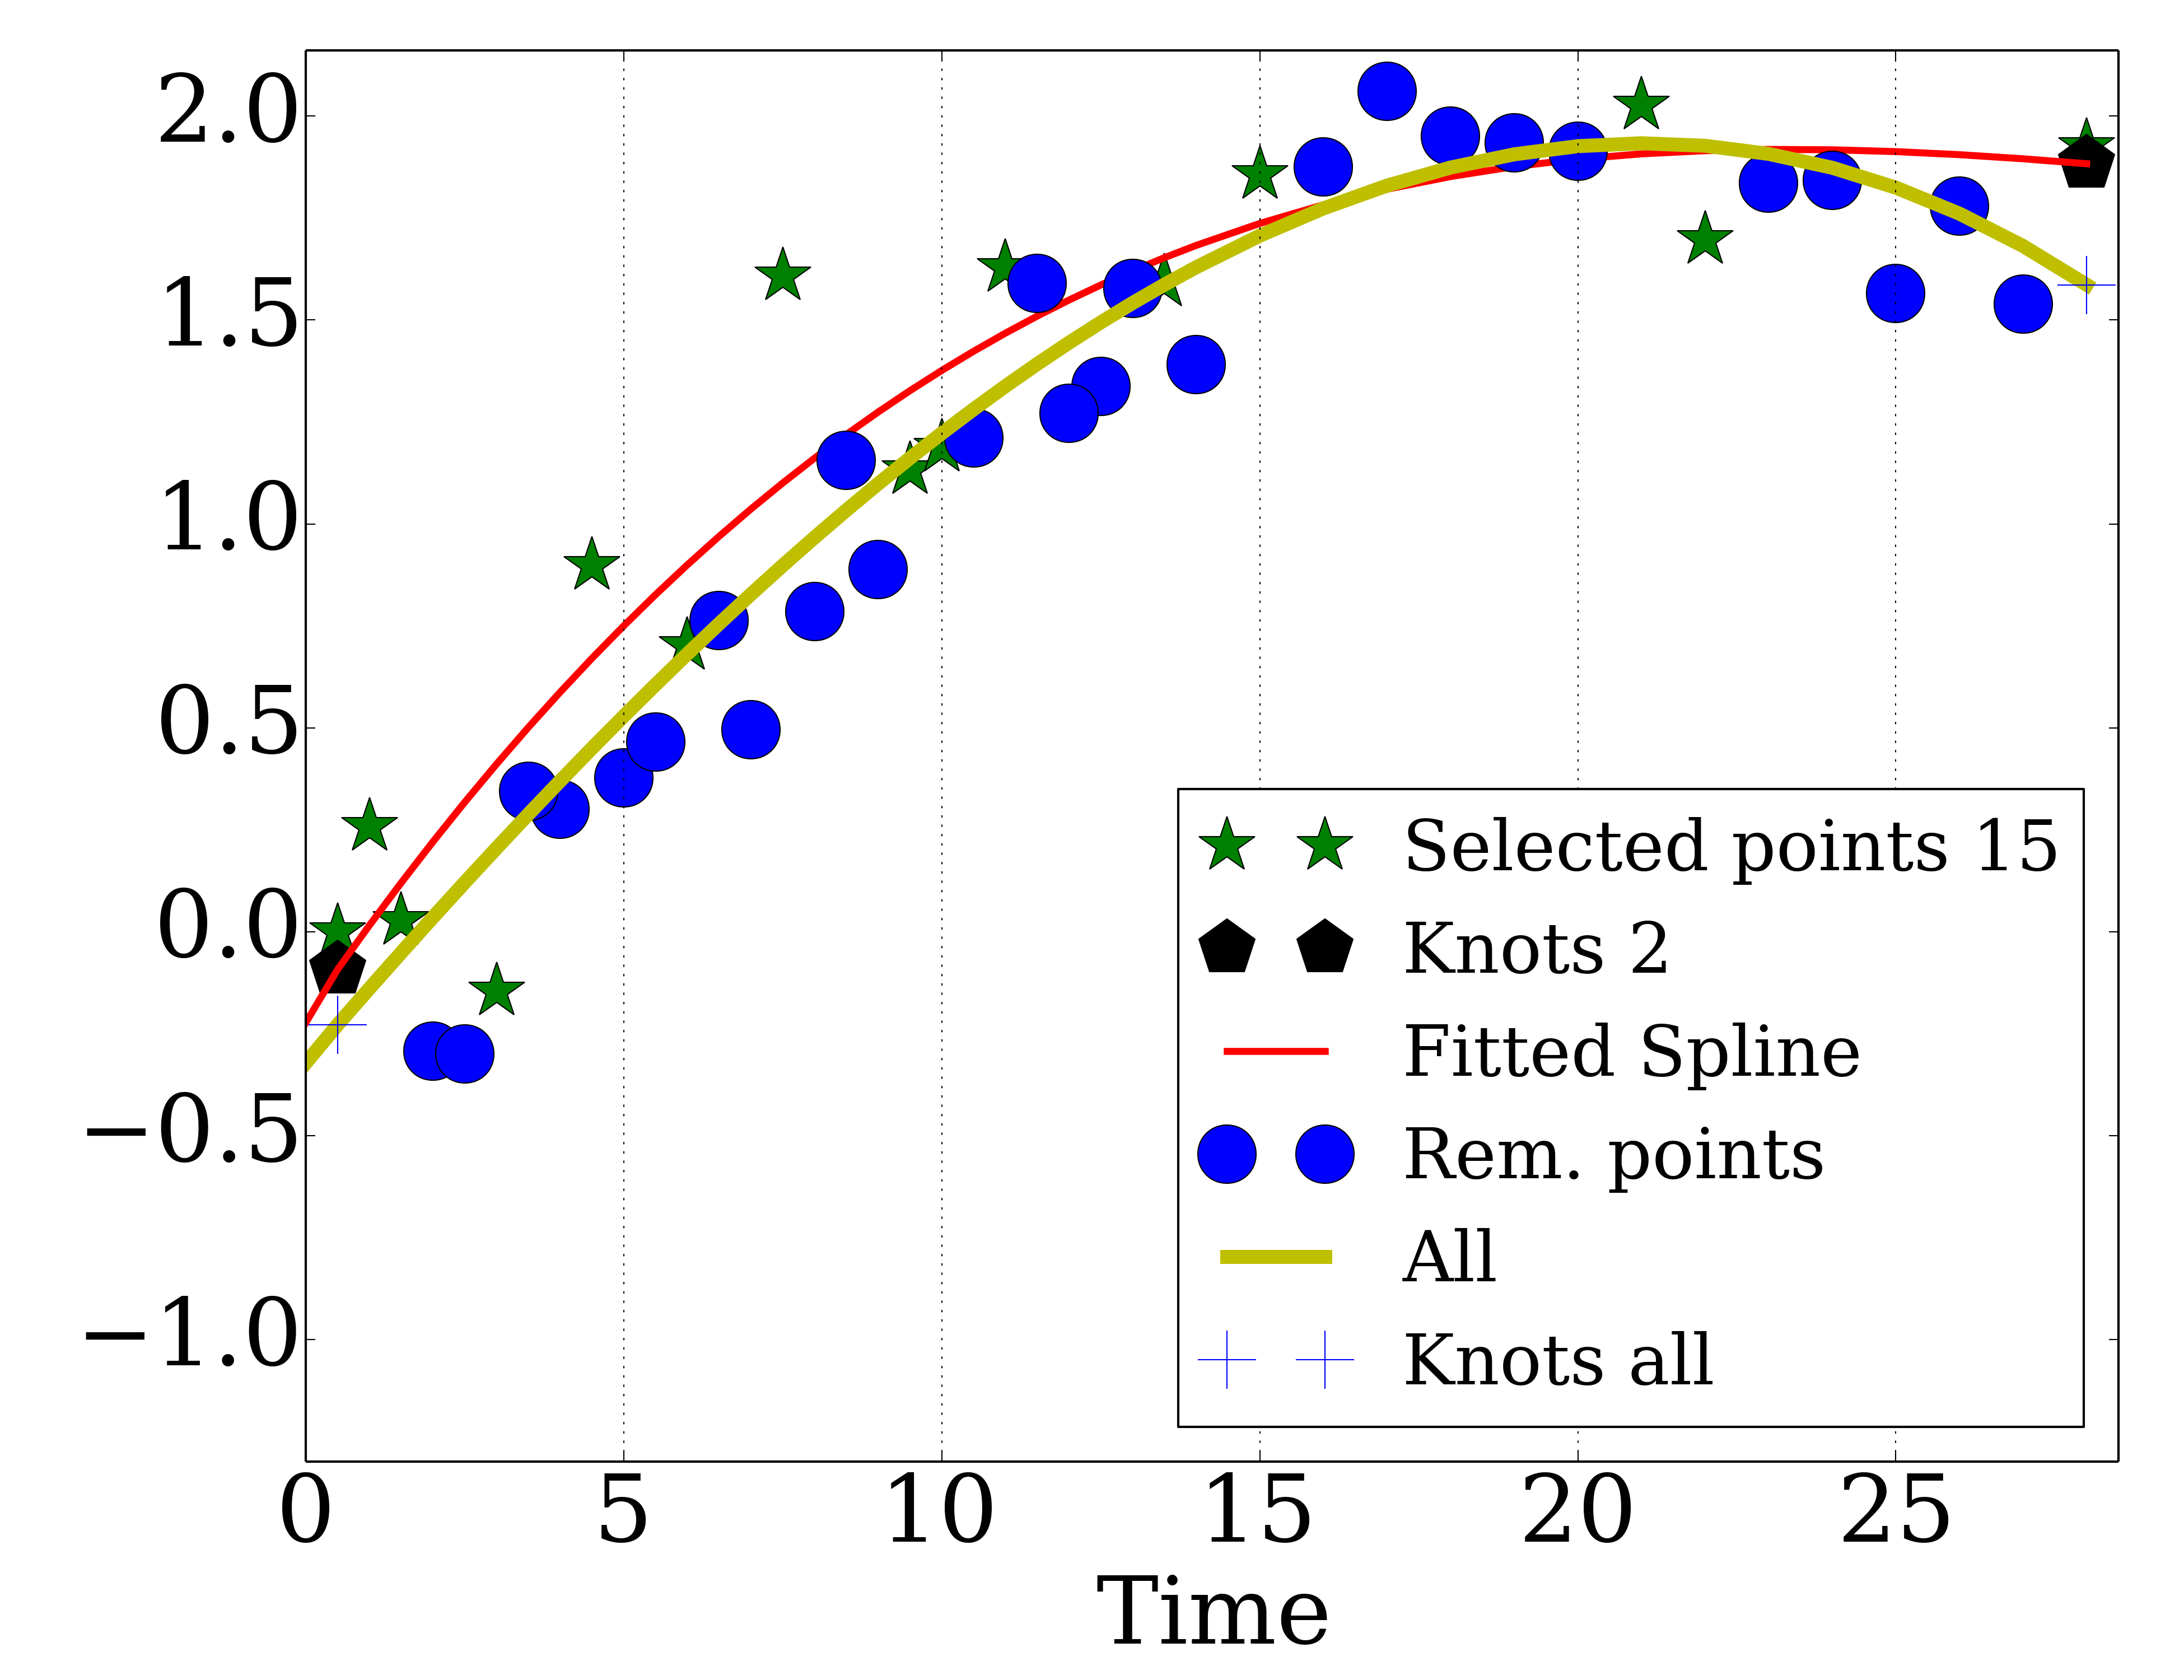
\includegraphics[scale=0.12]{{plots/newdata/splineplots15/PDGFRA_15_all}.png}}
\hfill
\subfloat[ELN]{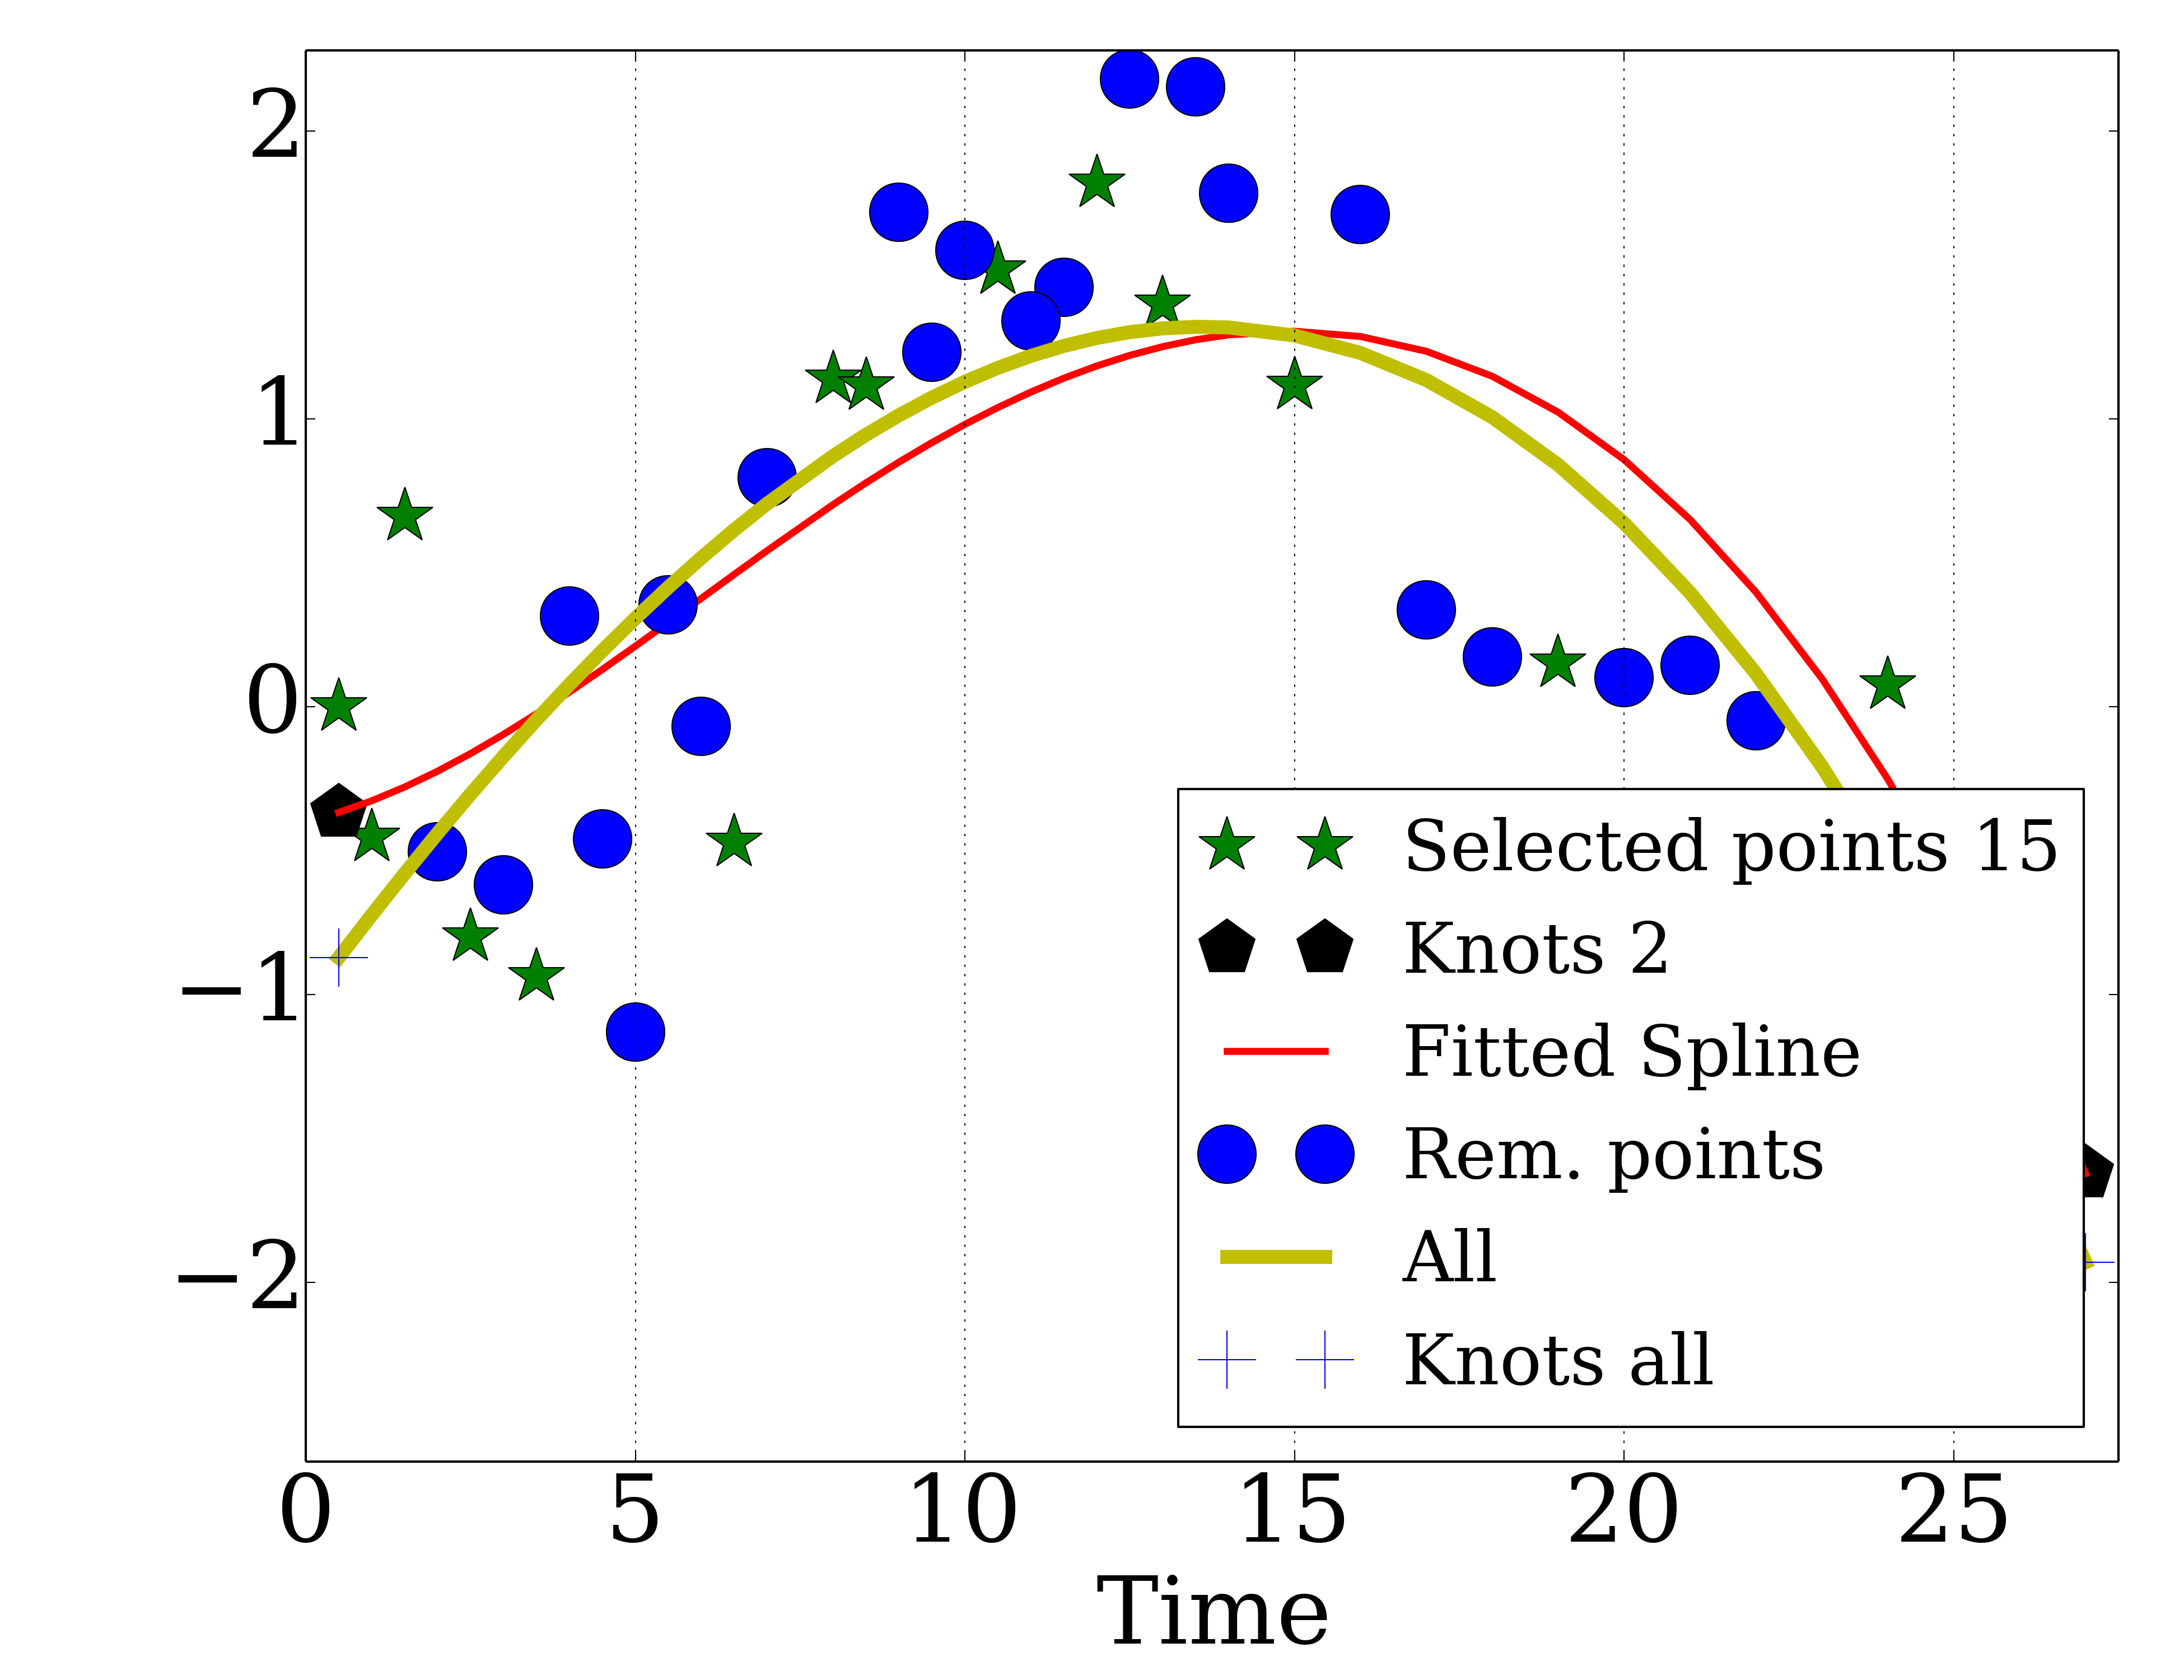
\includegraphics[scale=0.12]{{plots/newdata/splineplots15/Eln_15_all}.png}}
\hfill
\subfloat[INMT]{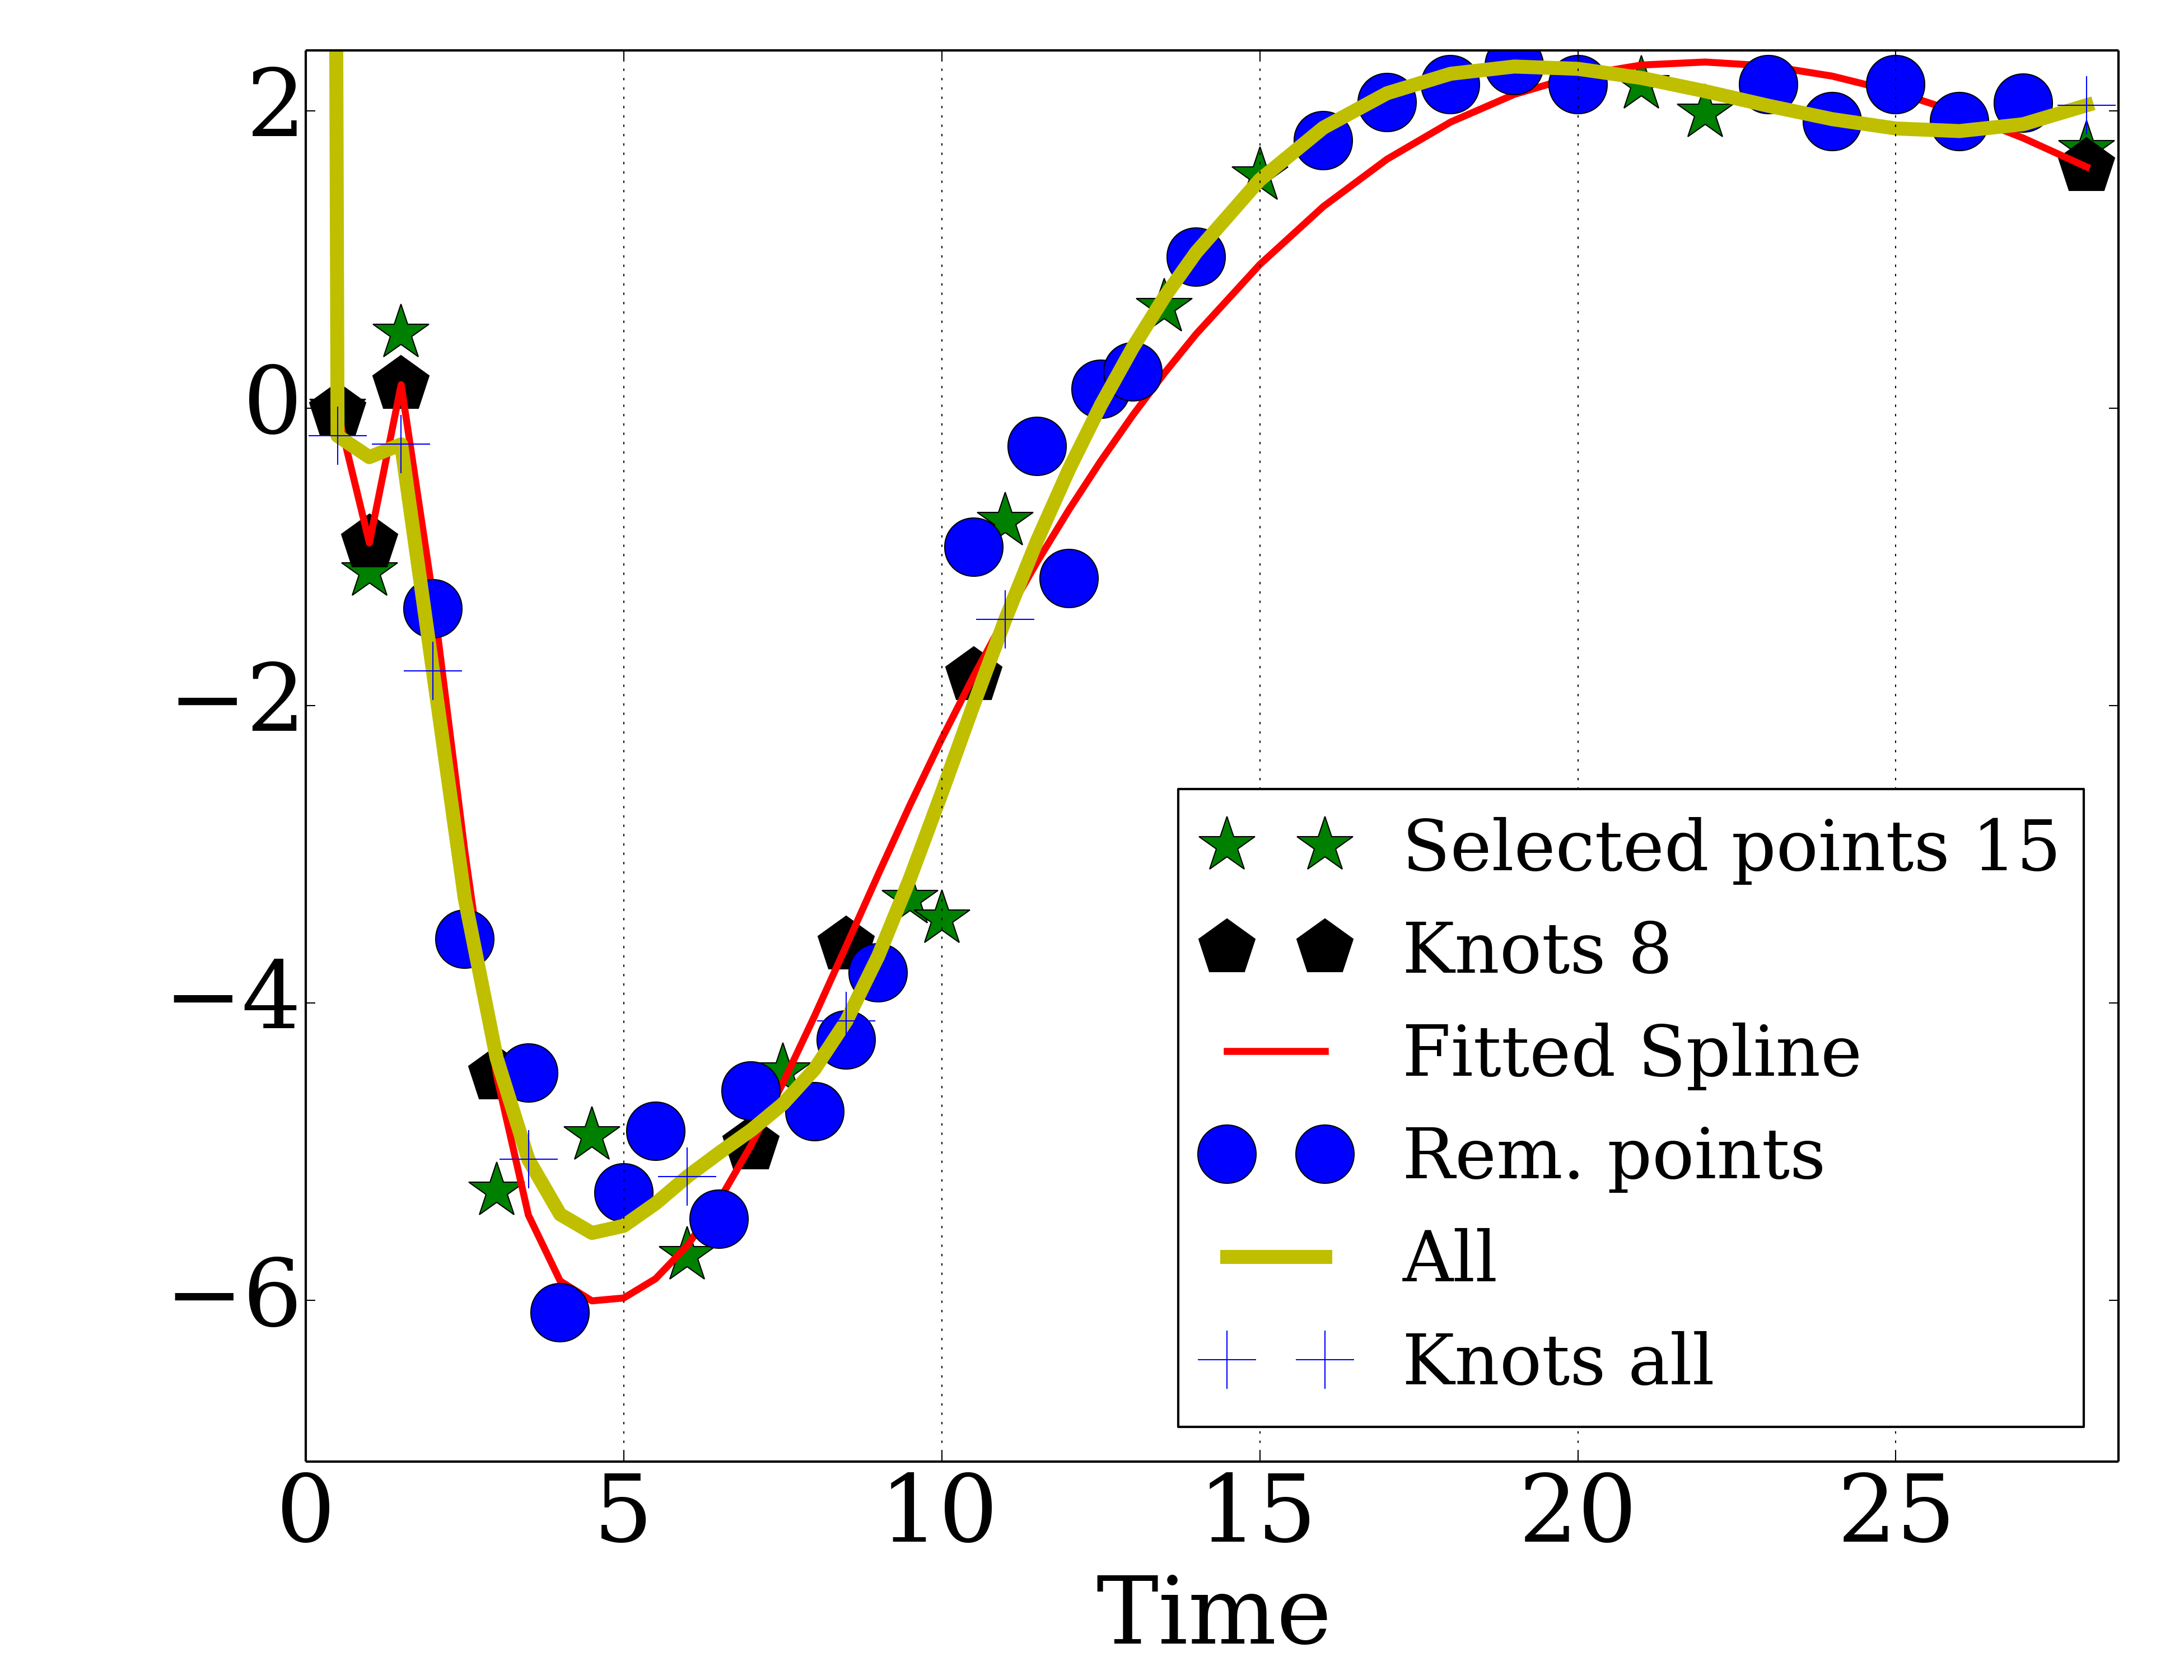
\includegraphics[scale=0.12]{{plots/newdata/splineplots15/INMT_15_all}.png}}
\hfill
\end{minipage}
\caption{Reconstructed expression profiles over genes a) PDGFRA, b) ELN, c) INMT}
\label{fig:centplots}
\end{figure}


\subsection{Identified time points over mRNA are predictive of miRNA profiles}\label{sec:mirnaexp}

%add mirna points also to plot
To test the usefulness of our method for predicting the correct sampling rates for other genomic datasets, we next profiled mouse
miRNAs for the same developmental process. miRNAs are important for
lung development as several miRNAs are differentially expressed
during lung development~\cite{williams2007} and some
miRNA families are involved in suppression of lung
tumors~\cite{kumar2008}. Unlike the mRNA dataset, which utilized prior knowledge to profile less than $1\%$ of
all genes, the miRNA dataset profiled $599$ miRNAs, more than $50\%$ of
known mouse miRNAs. Thus, such data represents an
unbiased sample and can provide information on whether using one
type of genomic data can be helpful for determining rates for other
types. 

To test the usefulness of our approach, we used the miRNA
expression values for the time points determined by the mRNA analysis to reconstruct the complete trajectories for each miRNA.
The results are presented in Figure~\ref{fig:mirnaerrplots}. In
addition to the comparison included in the mRNA figure, the miRNA
figure includes the optimal results for using miRNA data (as opposed
to mRNA data) to select the points. Even though the noise of miRNA data is
higher than mRNA dataset, relative ordering of the methods are almost
similar to Figure~\ref{fig:errplots}. As can be seen, the points selected by the mRNA analysis leads to
reconstruction that is much better than when using random points~($p <
0.01$) highlighting the relationship between the two datasets and the
ability to use one to determine points for the other. Further,
performance using the mRNA set is very similar to the performance
using the miRNA data itself. For example, when using the $13$
selected mRNA points, the average mean squared error is $0.4312$ whereas when
using the optimal points based on the miRNA data itself the error
 is $0.4042$. This serves as a strong indication that mRNAs can serve as a general proxy for
selecting time points.
%We also analyze the similarity of miRNA optimal points to mRNA optimal
%points as in Figure~\ref{xxx}.

\begin{figure}
\centering
\includegraphics[scale=0.25]{{plots/mirnadata/perform}.png}
\caption{Performance of \Tempselect by increasing number of selected
  points over miRNA dataset}
\label{fig:mirnaerrplots}
\end{figure}

Figure~\ref{fig:mirnaplots_spec} presents the reconstructed and measured
expression values for a few miRNAs using time points identified over
mRNA dataset. Accurate prediction of different miRNA profiles show the importance of
identified points over mRNA dataset. Among these miRNAs, mmu-miR-100
targets Fgfr3 and Igf1r, mmu-miR-136 targets Tgfb2. Similarly, mmu-miR-152 targets Meox2,
Robo1, Fbn1, Nfya. Lastly, mmu-miR-219 targets PDGFRA, Eya2, Esr1,
Esr2, Efnb2 and Robo1 some of which are associated with BPD in preterm
infants~\cite{popova2014}. 
%Spline-based reconstruction performs better than linear reconstruction similar to mRNA dataset.

\begin{figure}[ht]
\centering
\begin{minipage}{1.0\textwidth}
\subfloat[mmu-miR-100]{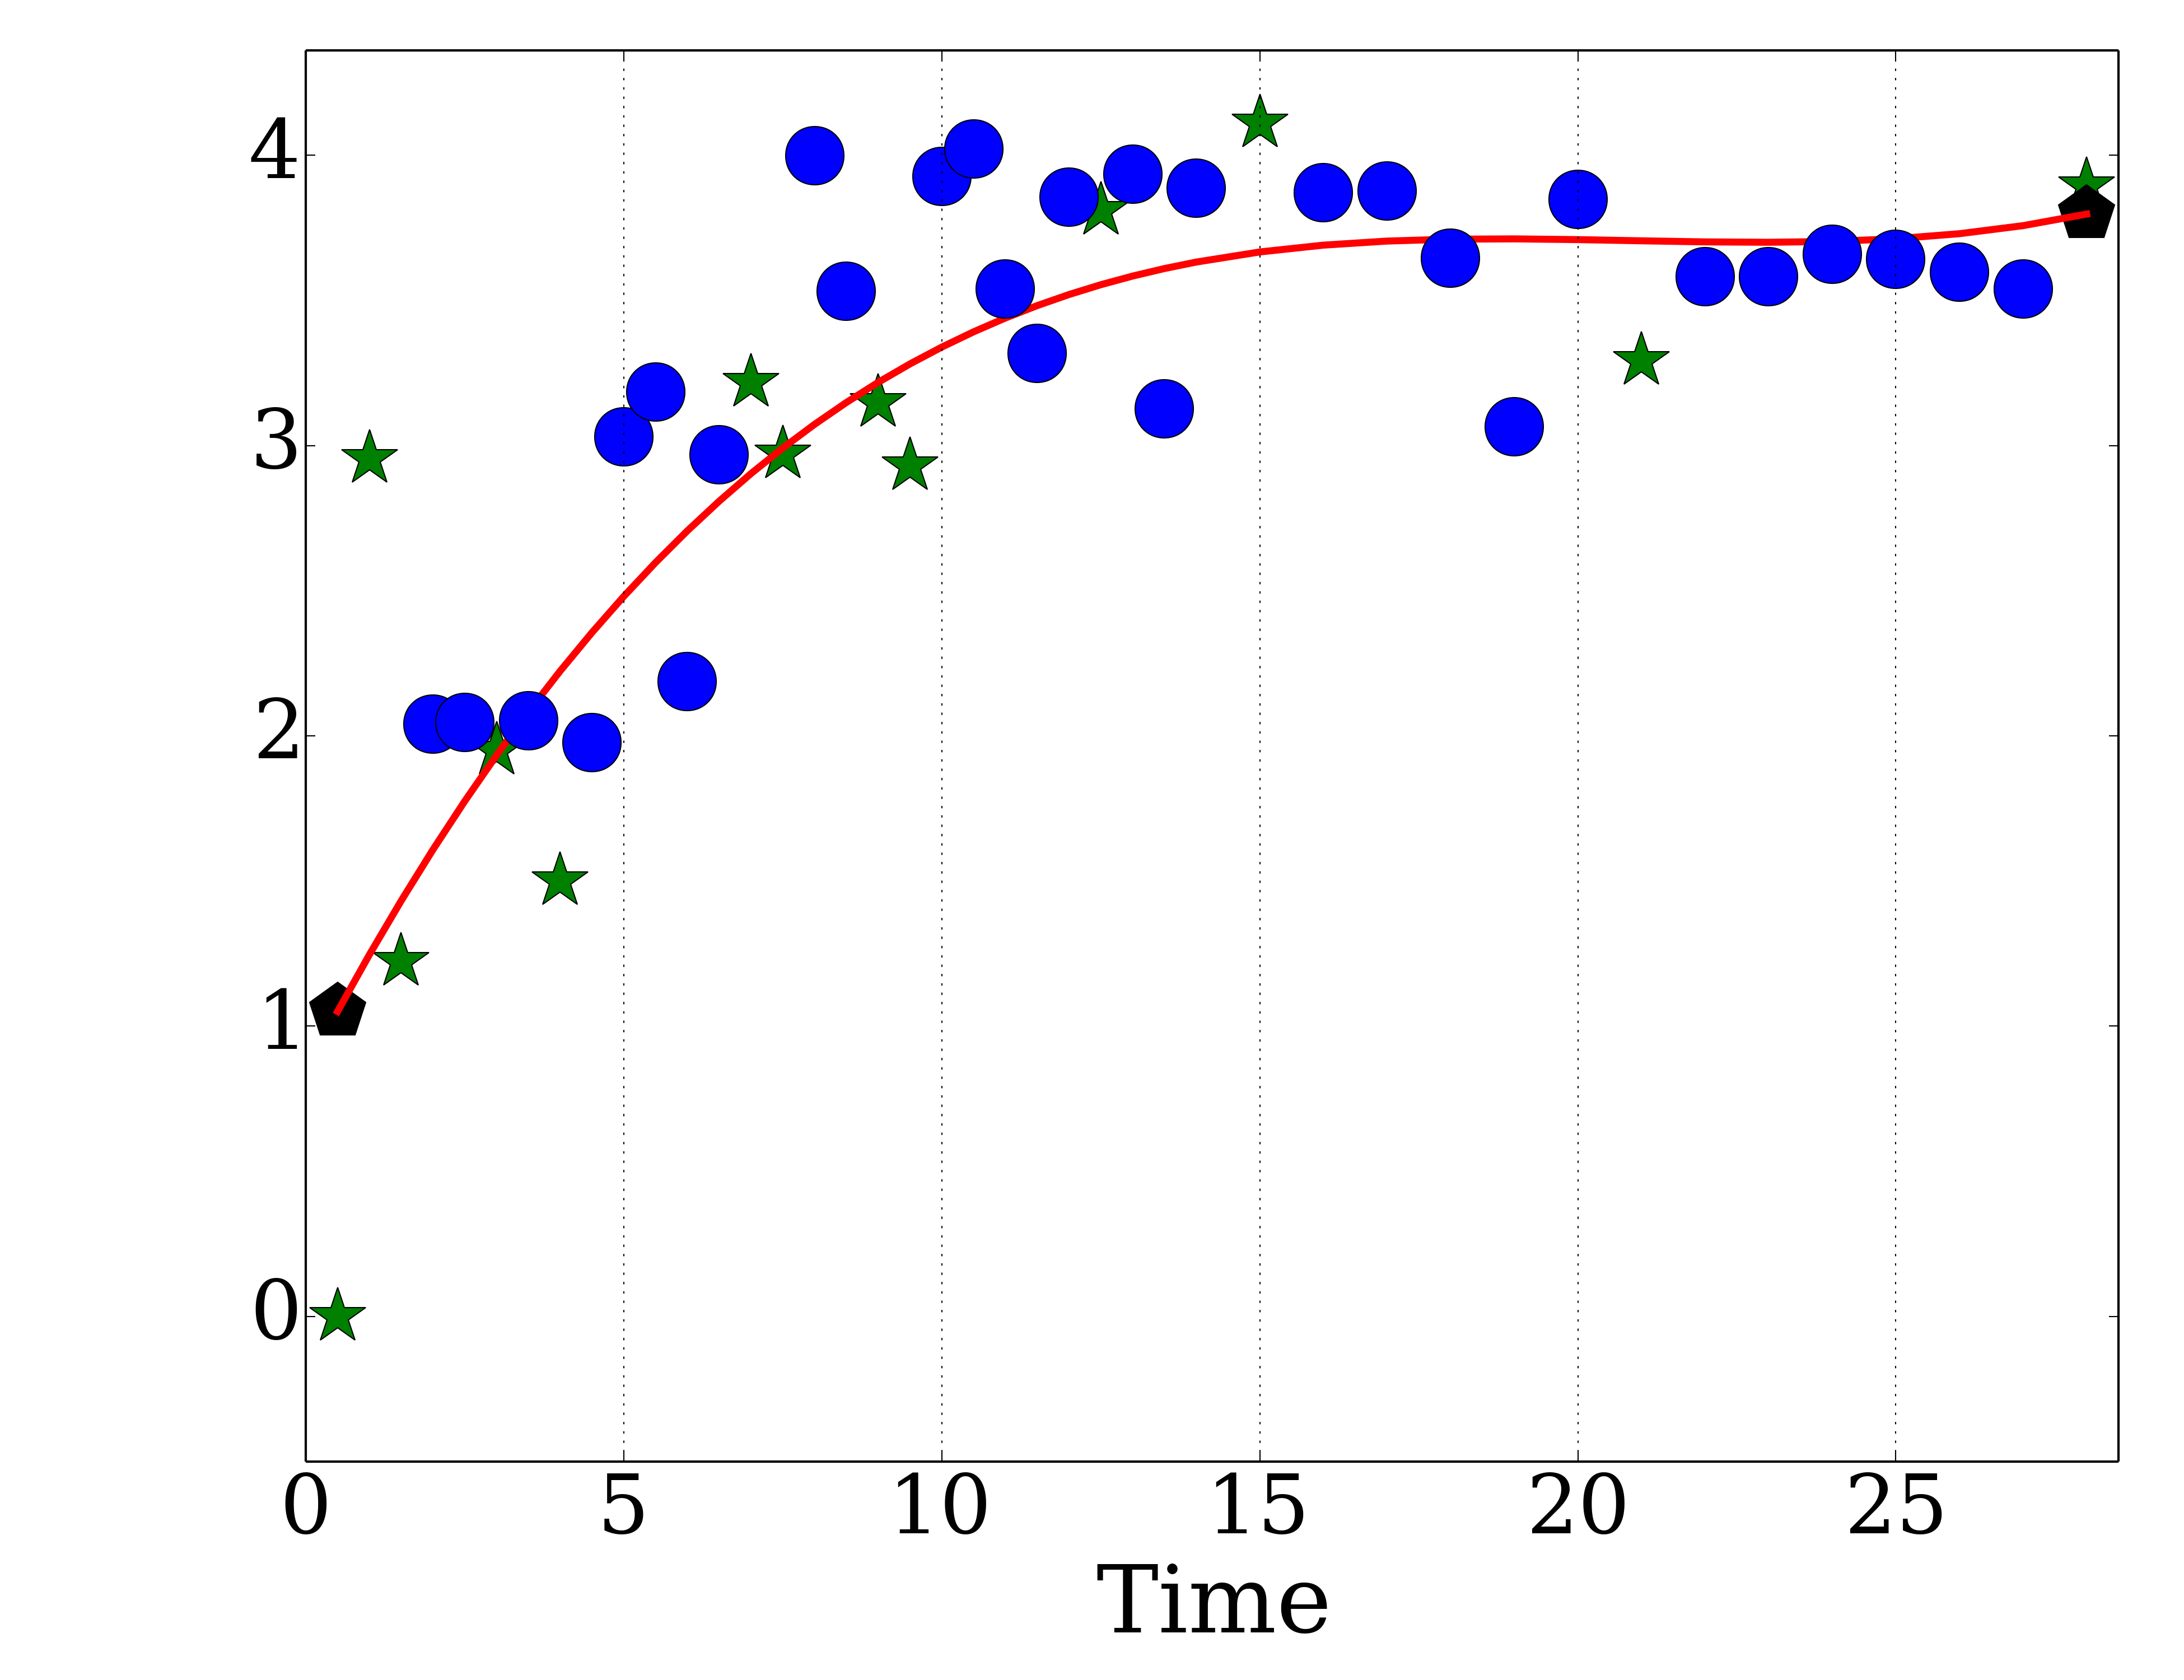
\includegraphics[scale=0.15]{{plots/mirnadata/splineplots13/uni/mmu-miR-100_13}.png}}
\hfill
\subfloat[mmu-miR-136]{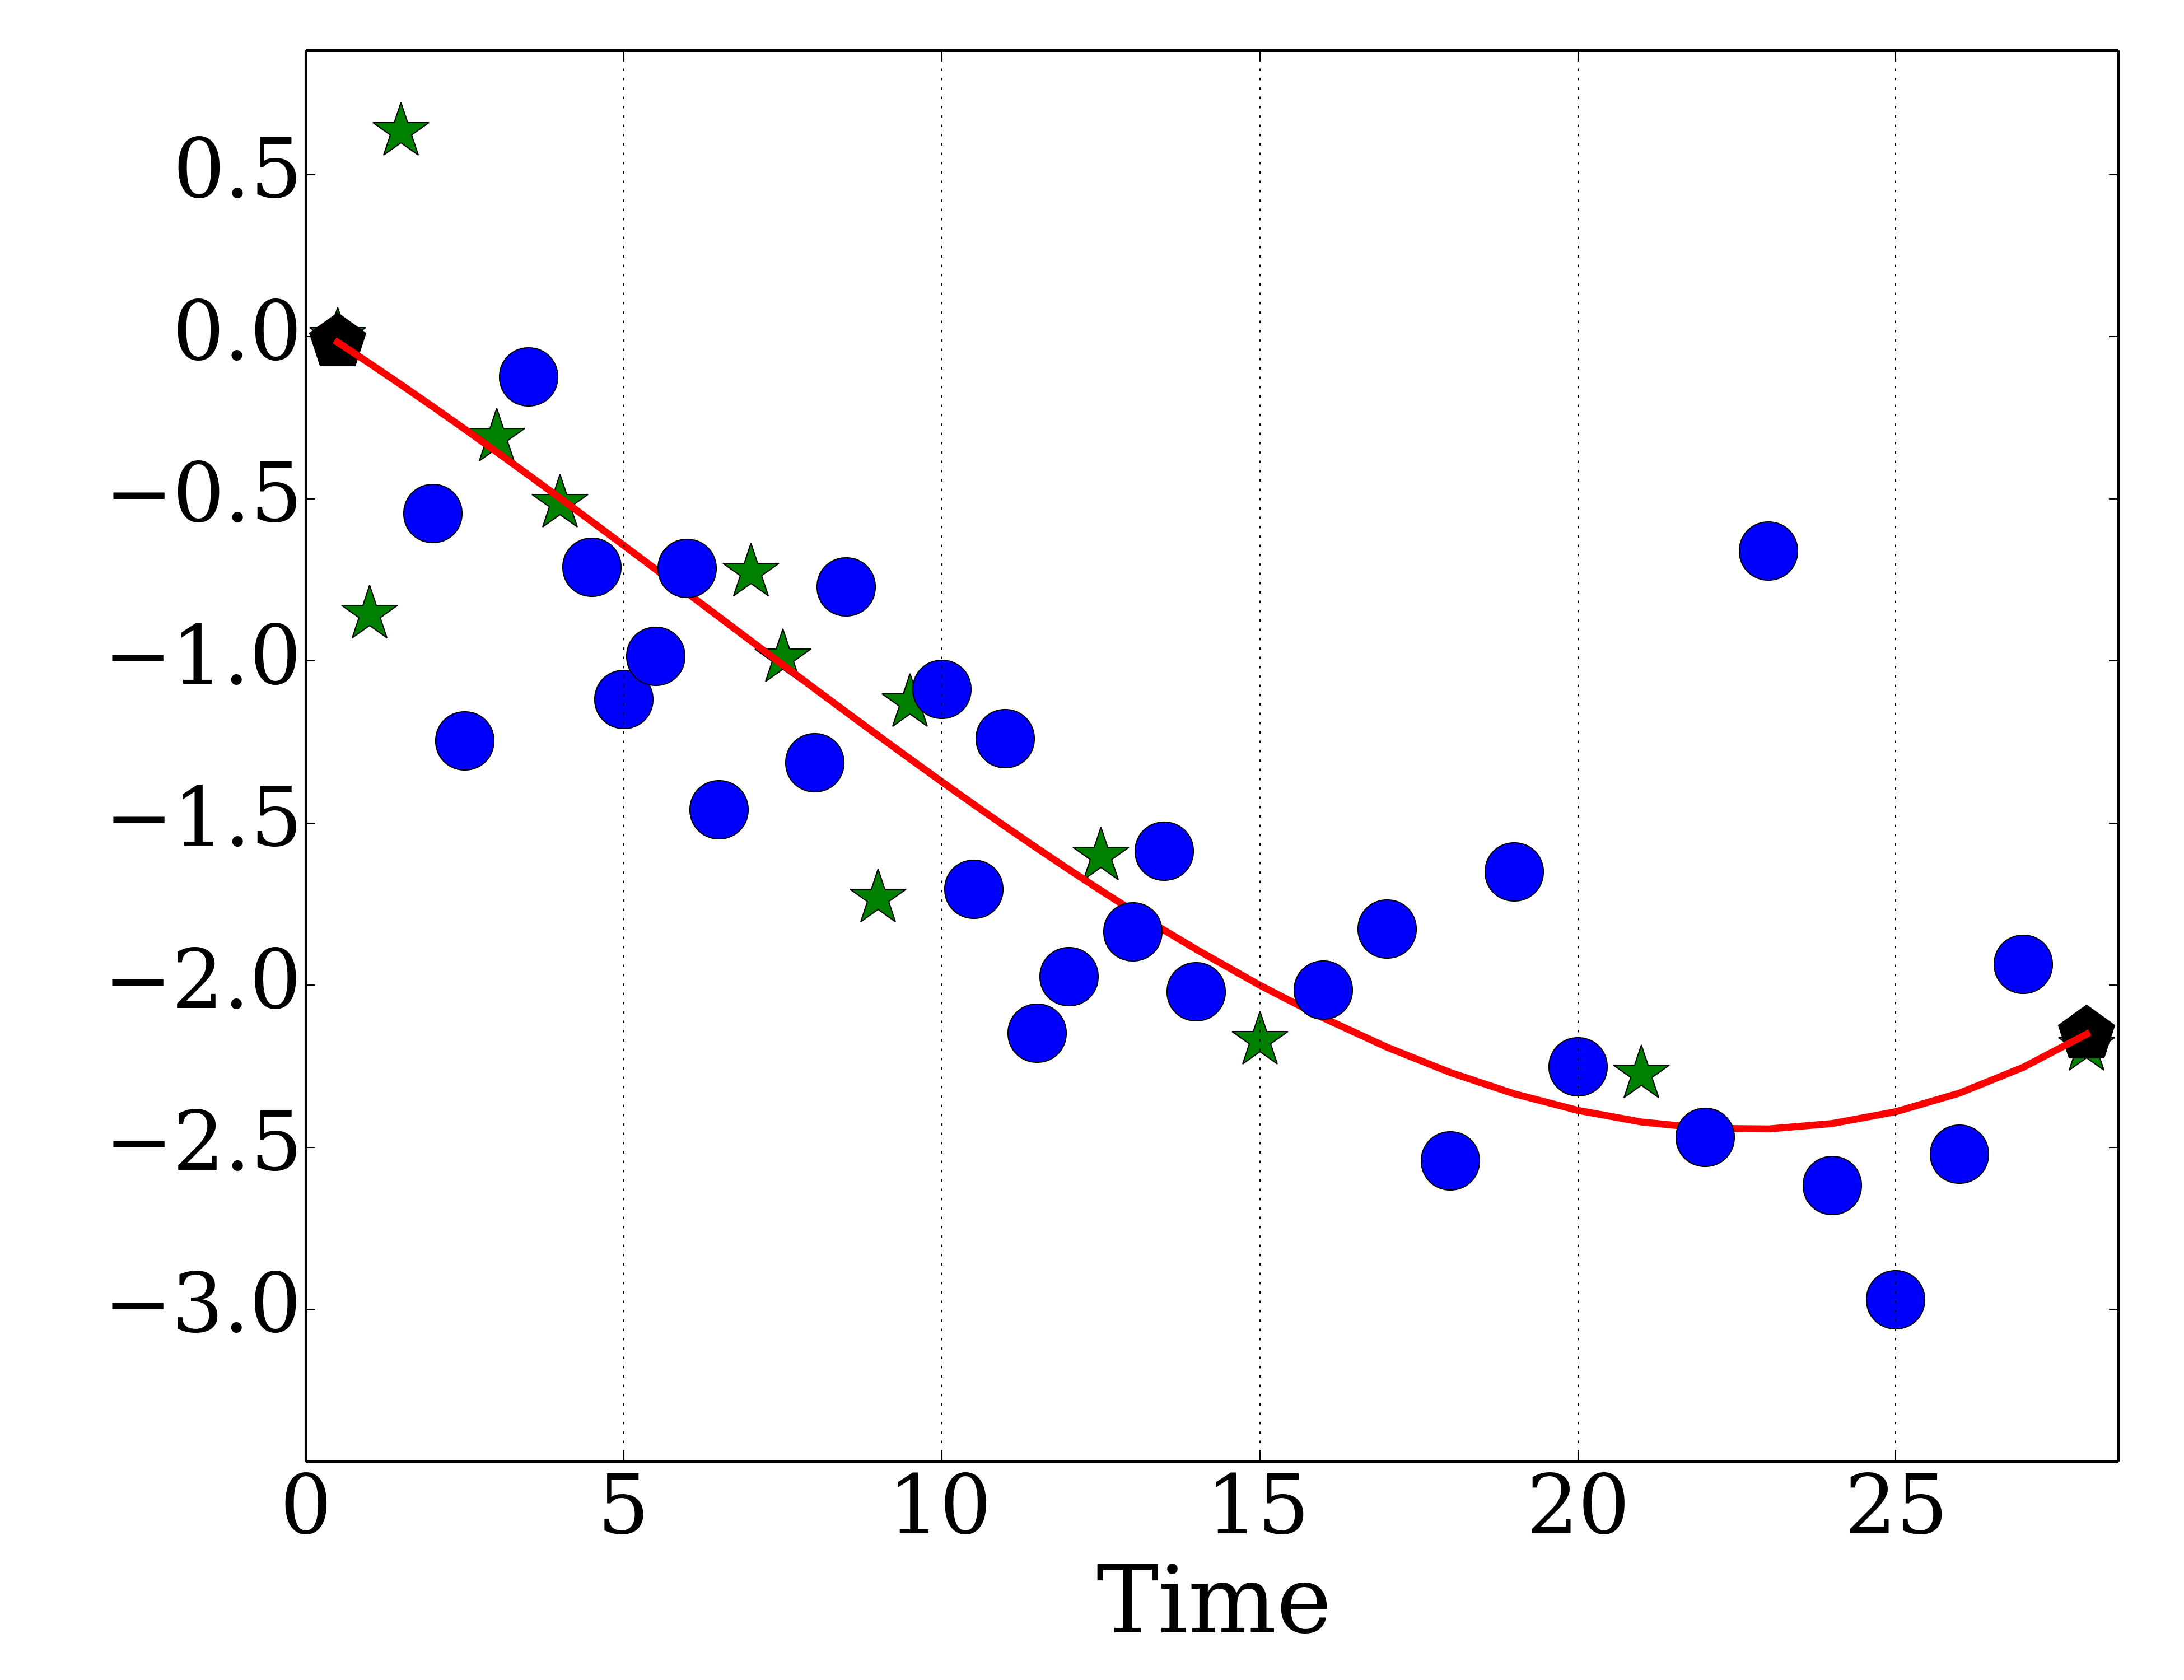
\includegraphics[scale=0.15]{{plots/mirnadata/splineplots13/uni/mmu-miR-136_13}.png}}
\\
\centering
\hfill
\subfloat[mmu-miR-152]{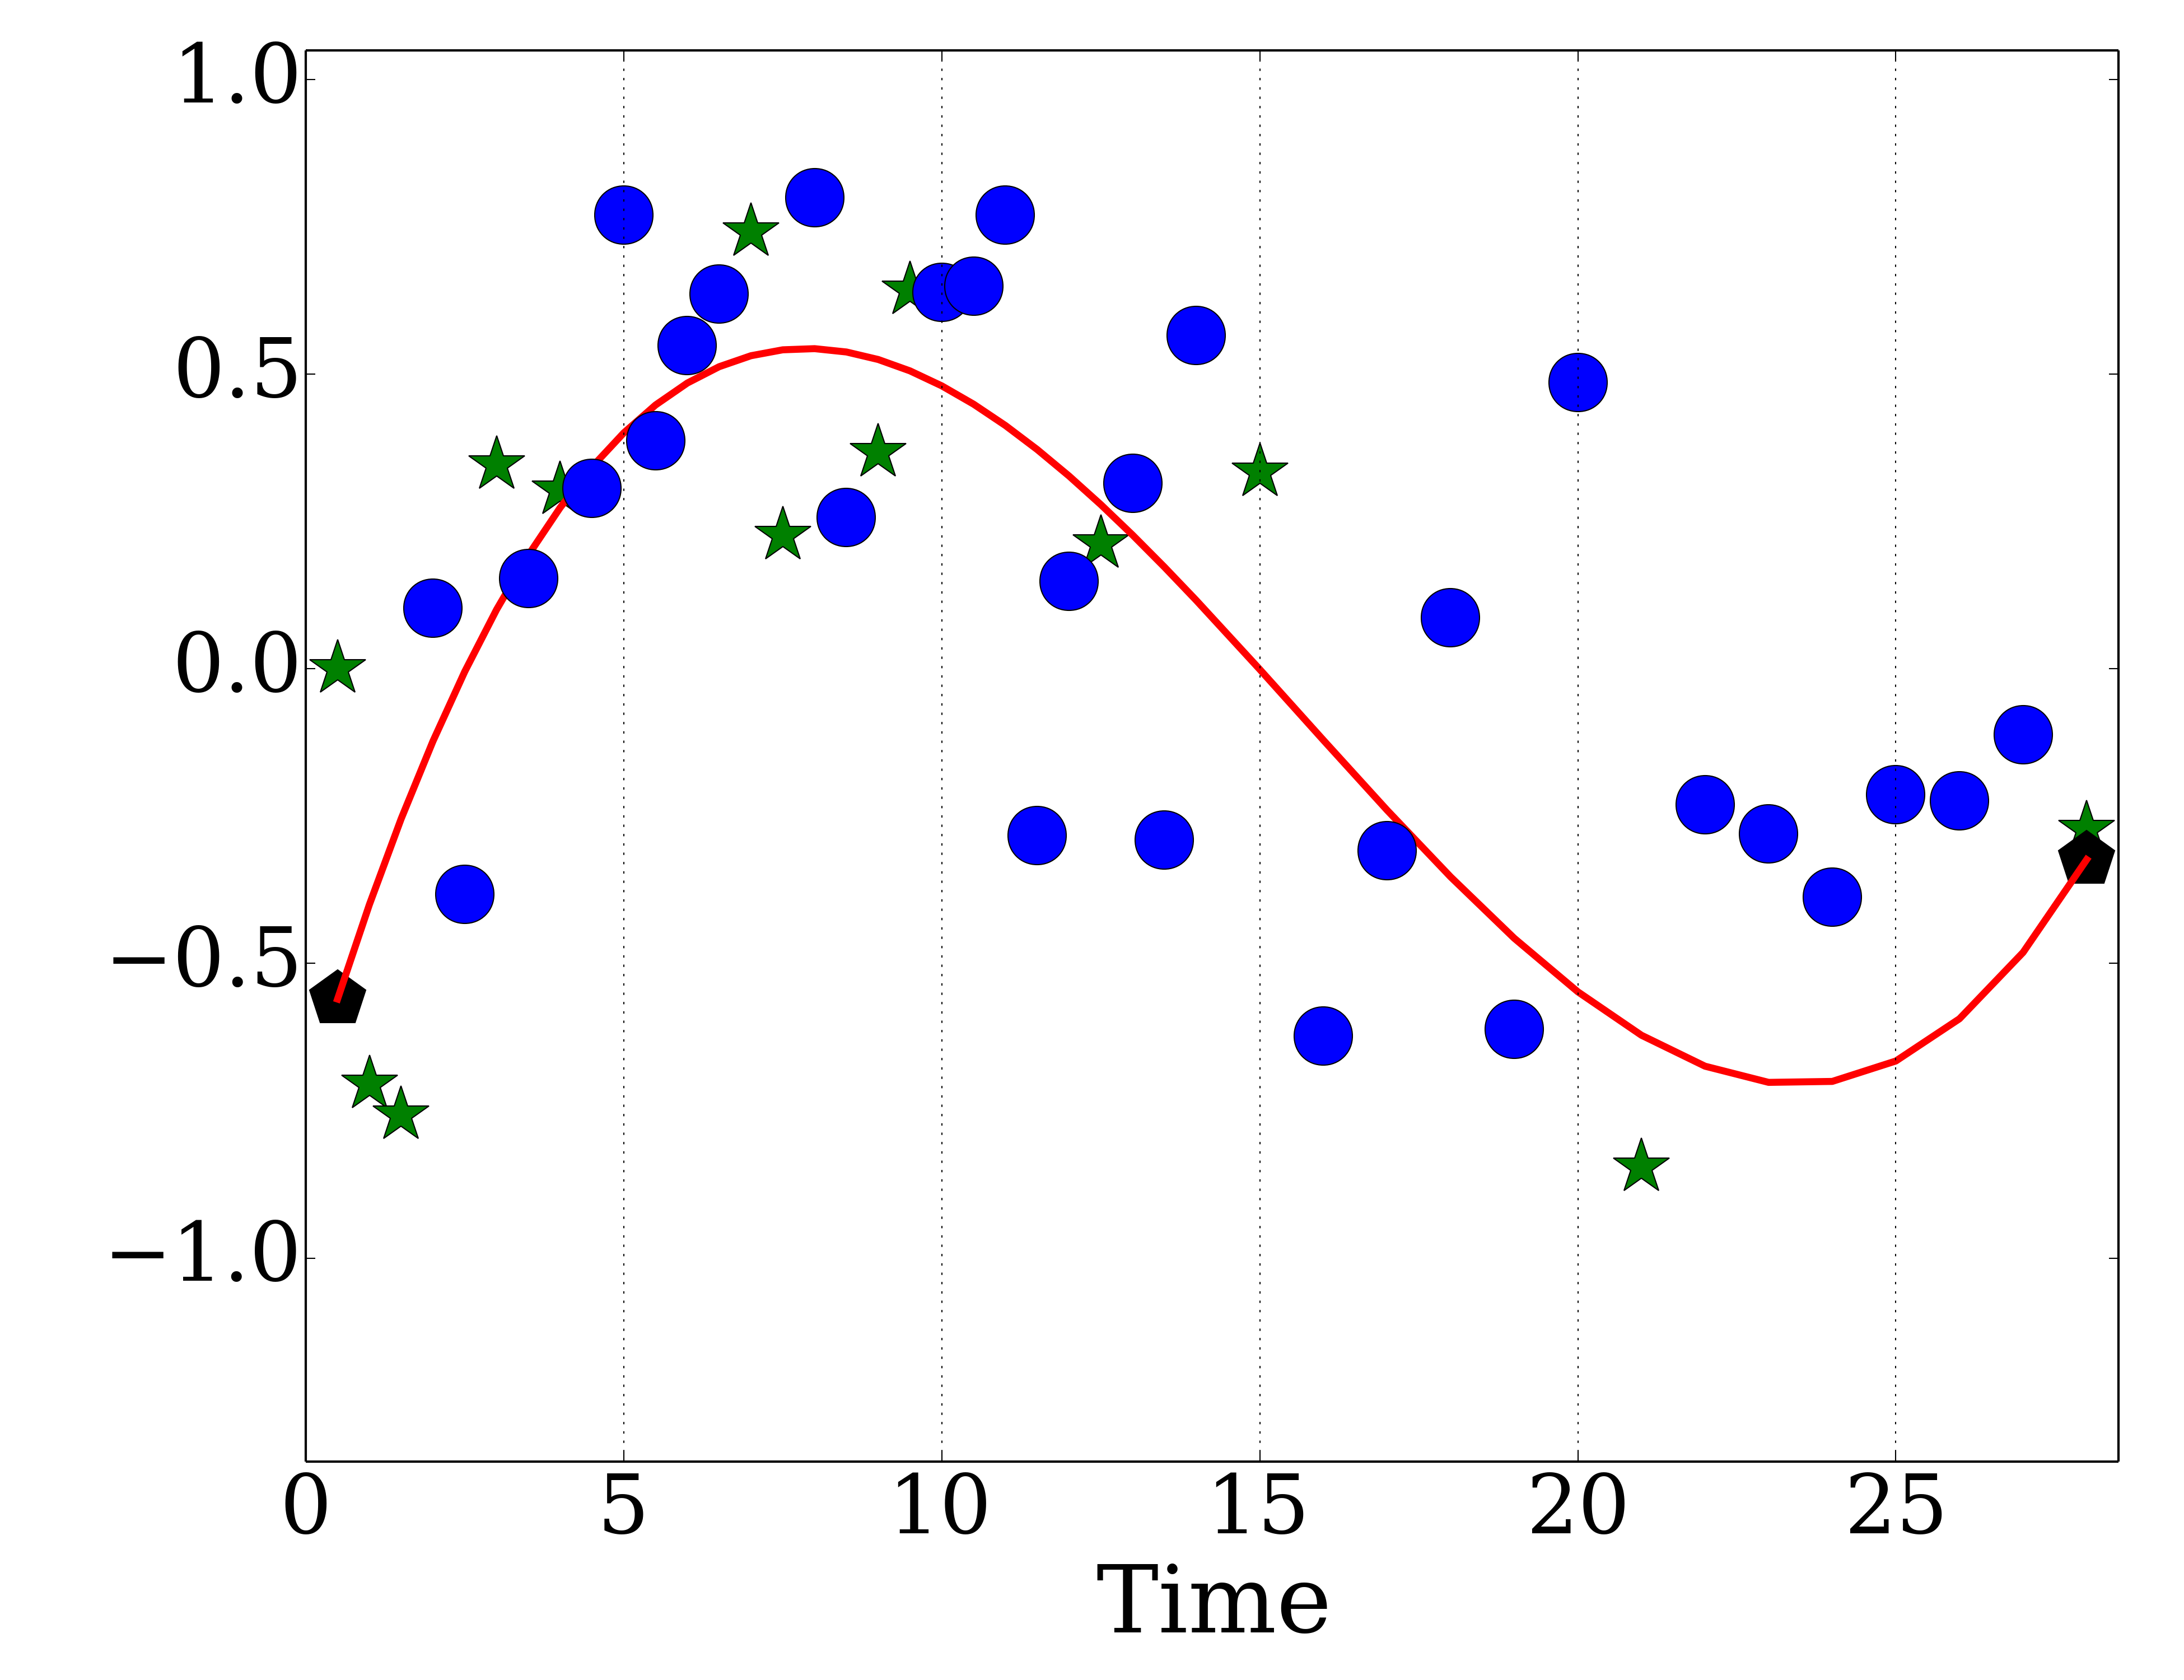
\includegraphics[scale=0.15]{{plots/mirnadata/splineplots13/uni/mmu-miR-152_13}.png}}
\hfill
\subfloat[mmu-miR-219]{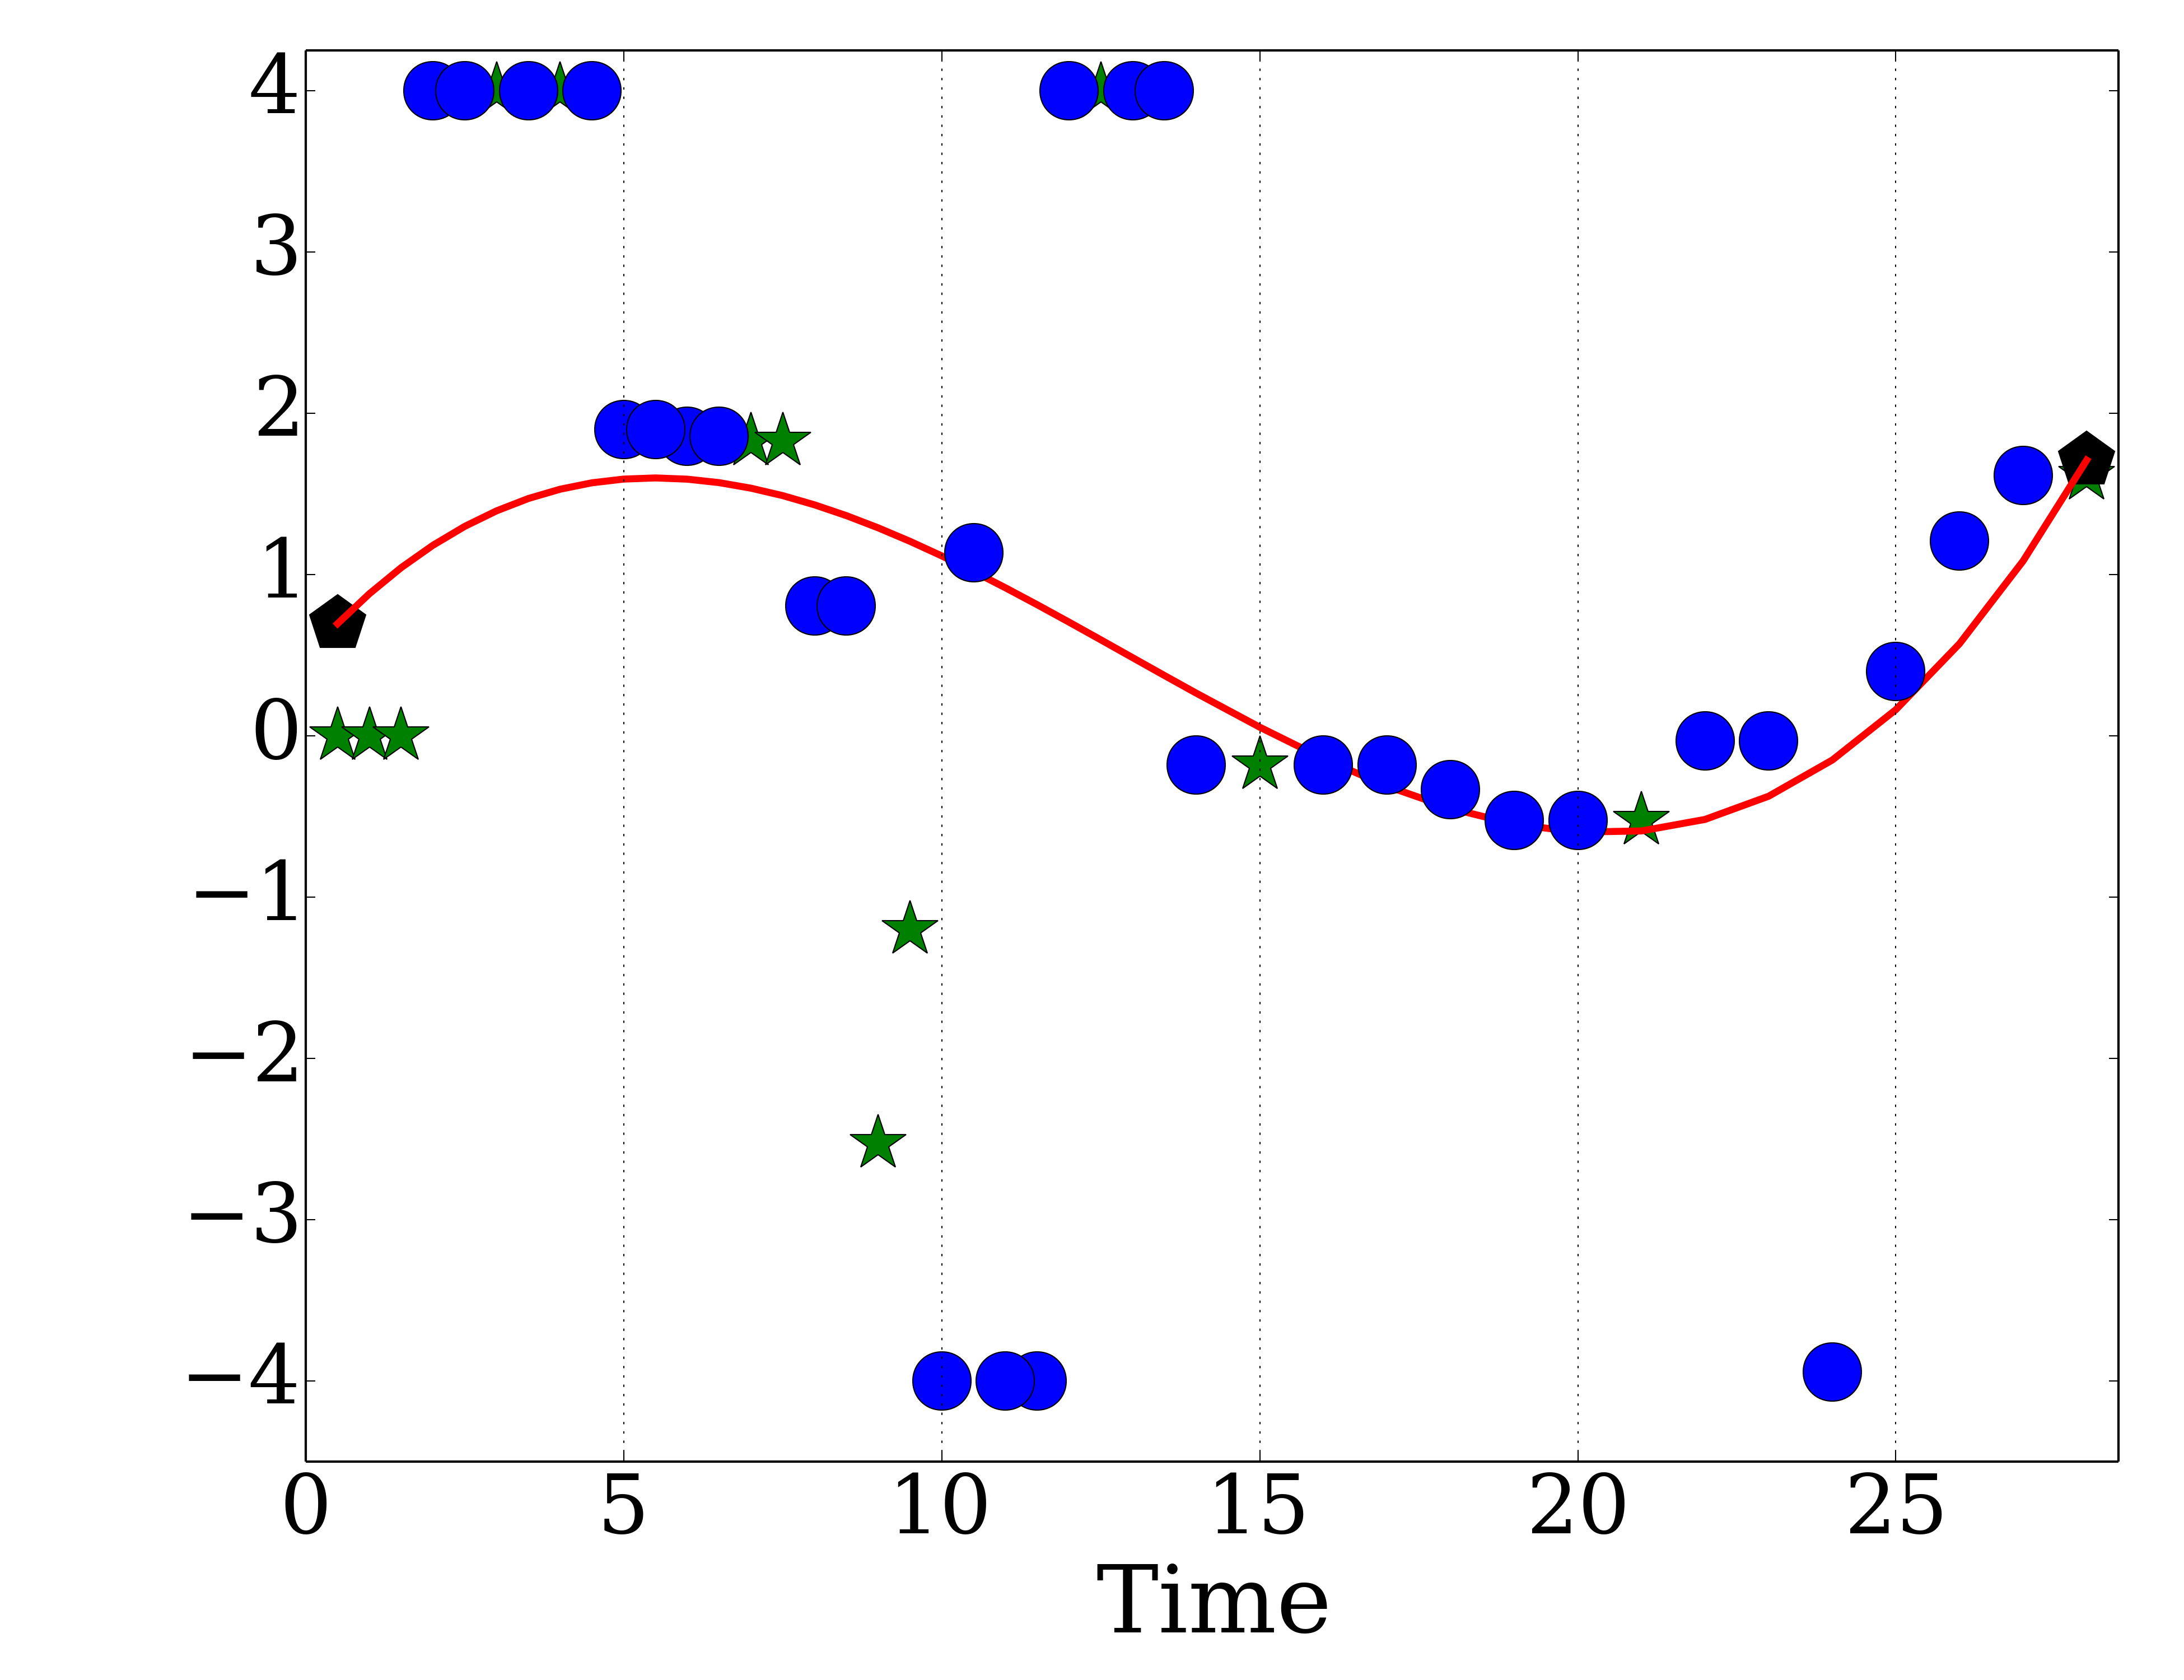
\includegraphics[scale=0.15]{{plots/mirnadata/splineplots13/uni/mmu-miR-219_13}.png}}
\end{minipage}
\caption{Predicted expression profiles of miRNAs a) mmu-miR-100, b)
  mmu-miR-136, c) mmu-miR-152, d) mmu-miR-219.}
\label{fig:mirnaplots_spec}
\end{figure}


\subsection{miRNA Clusters Are Enriched For Several Biological Processes}\label{sec:mirna}

Detailed analysis of miRNA dataset shows clustered expression profiles
of miRNAs as in Figure~\ref{fig:clustmirna}. We identified $8$ stable miRNA
clusters by k-means algorithm~\cite{kmeans} where the number of clusters is selected by
Bayesian Information Criteria~\cite{bic}. We find clusters to change more frequently
than mRNA data as miRNA is noisier than mRNA data~(See Supplementary
Figure~\ref{fig:sup6} for mRNA clusters). After mapping each miRNA to
the set of corresponding genes by TargetScan~\cite{agarwal2015}, we run
gene-enrichment analysis by FuncAssociate~\cite{berriz2003}. We find clusters to be enriched
for several Gene Ontology biological processes~\cite{go}. For
instance, cluster $4$ is enriched for single-organism cellular
process, positive regulation of biological process, regulation of
metabolic process, etc.

\begin{figure}
\centering
\includegraphics[scale=0.2]{{plots/mirnadata/centplot}.png}
\caption{$8$ stable clusters}
\label{fig:clustmirna}
\end{figure}

\subsection{Comparison of Temporal Methylation Data With The Expression Data}\label{sec:compareboth}

%These points look more uniform than
%the $13$ points identified over gene-expression dataset which can be due
%to its lower sampling rate than expression profiles.
\Tempselect identified $0.5$, $5$, $15$, $26$ as candidate points out
of $8$ time points over temporal methylation data when we consider
each locus independently. When we only use the same $8$ time points over
gene-expression dataset, we also identified $0.5$, $5$, $15$, $26$ by running
\Tempselect over all subset of possible time points. We have also
observed similarity between both datasets by plotting them jointly as in Figure~\ref{fig:methgene} for DNMT3A, SRC,
and LOX genes. Among the multiple methylation loci belonging to a gene, we select
the most similar one in terms of pearson correlation~(See
Supplementary Table~\ref{tab:sup2} for correlation analysis). Overall,
similarity of the identified points when combined with the similarity
of the curves in the Figure suggest the possibility of global set of time points that are important for both genomic and epigenetic experiments.

\begin{figure}
\centering
\begin{minipage}{1.0\textwidth}
\subfloat[DNMT3A]{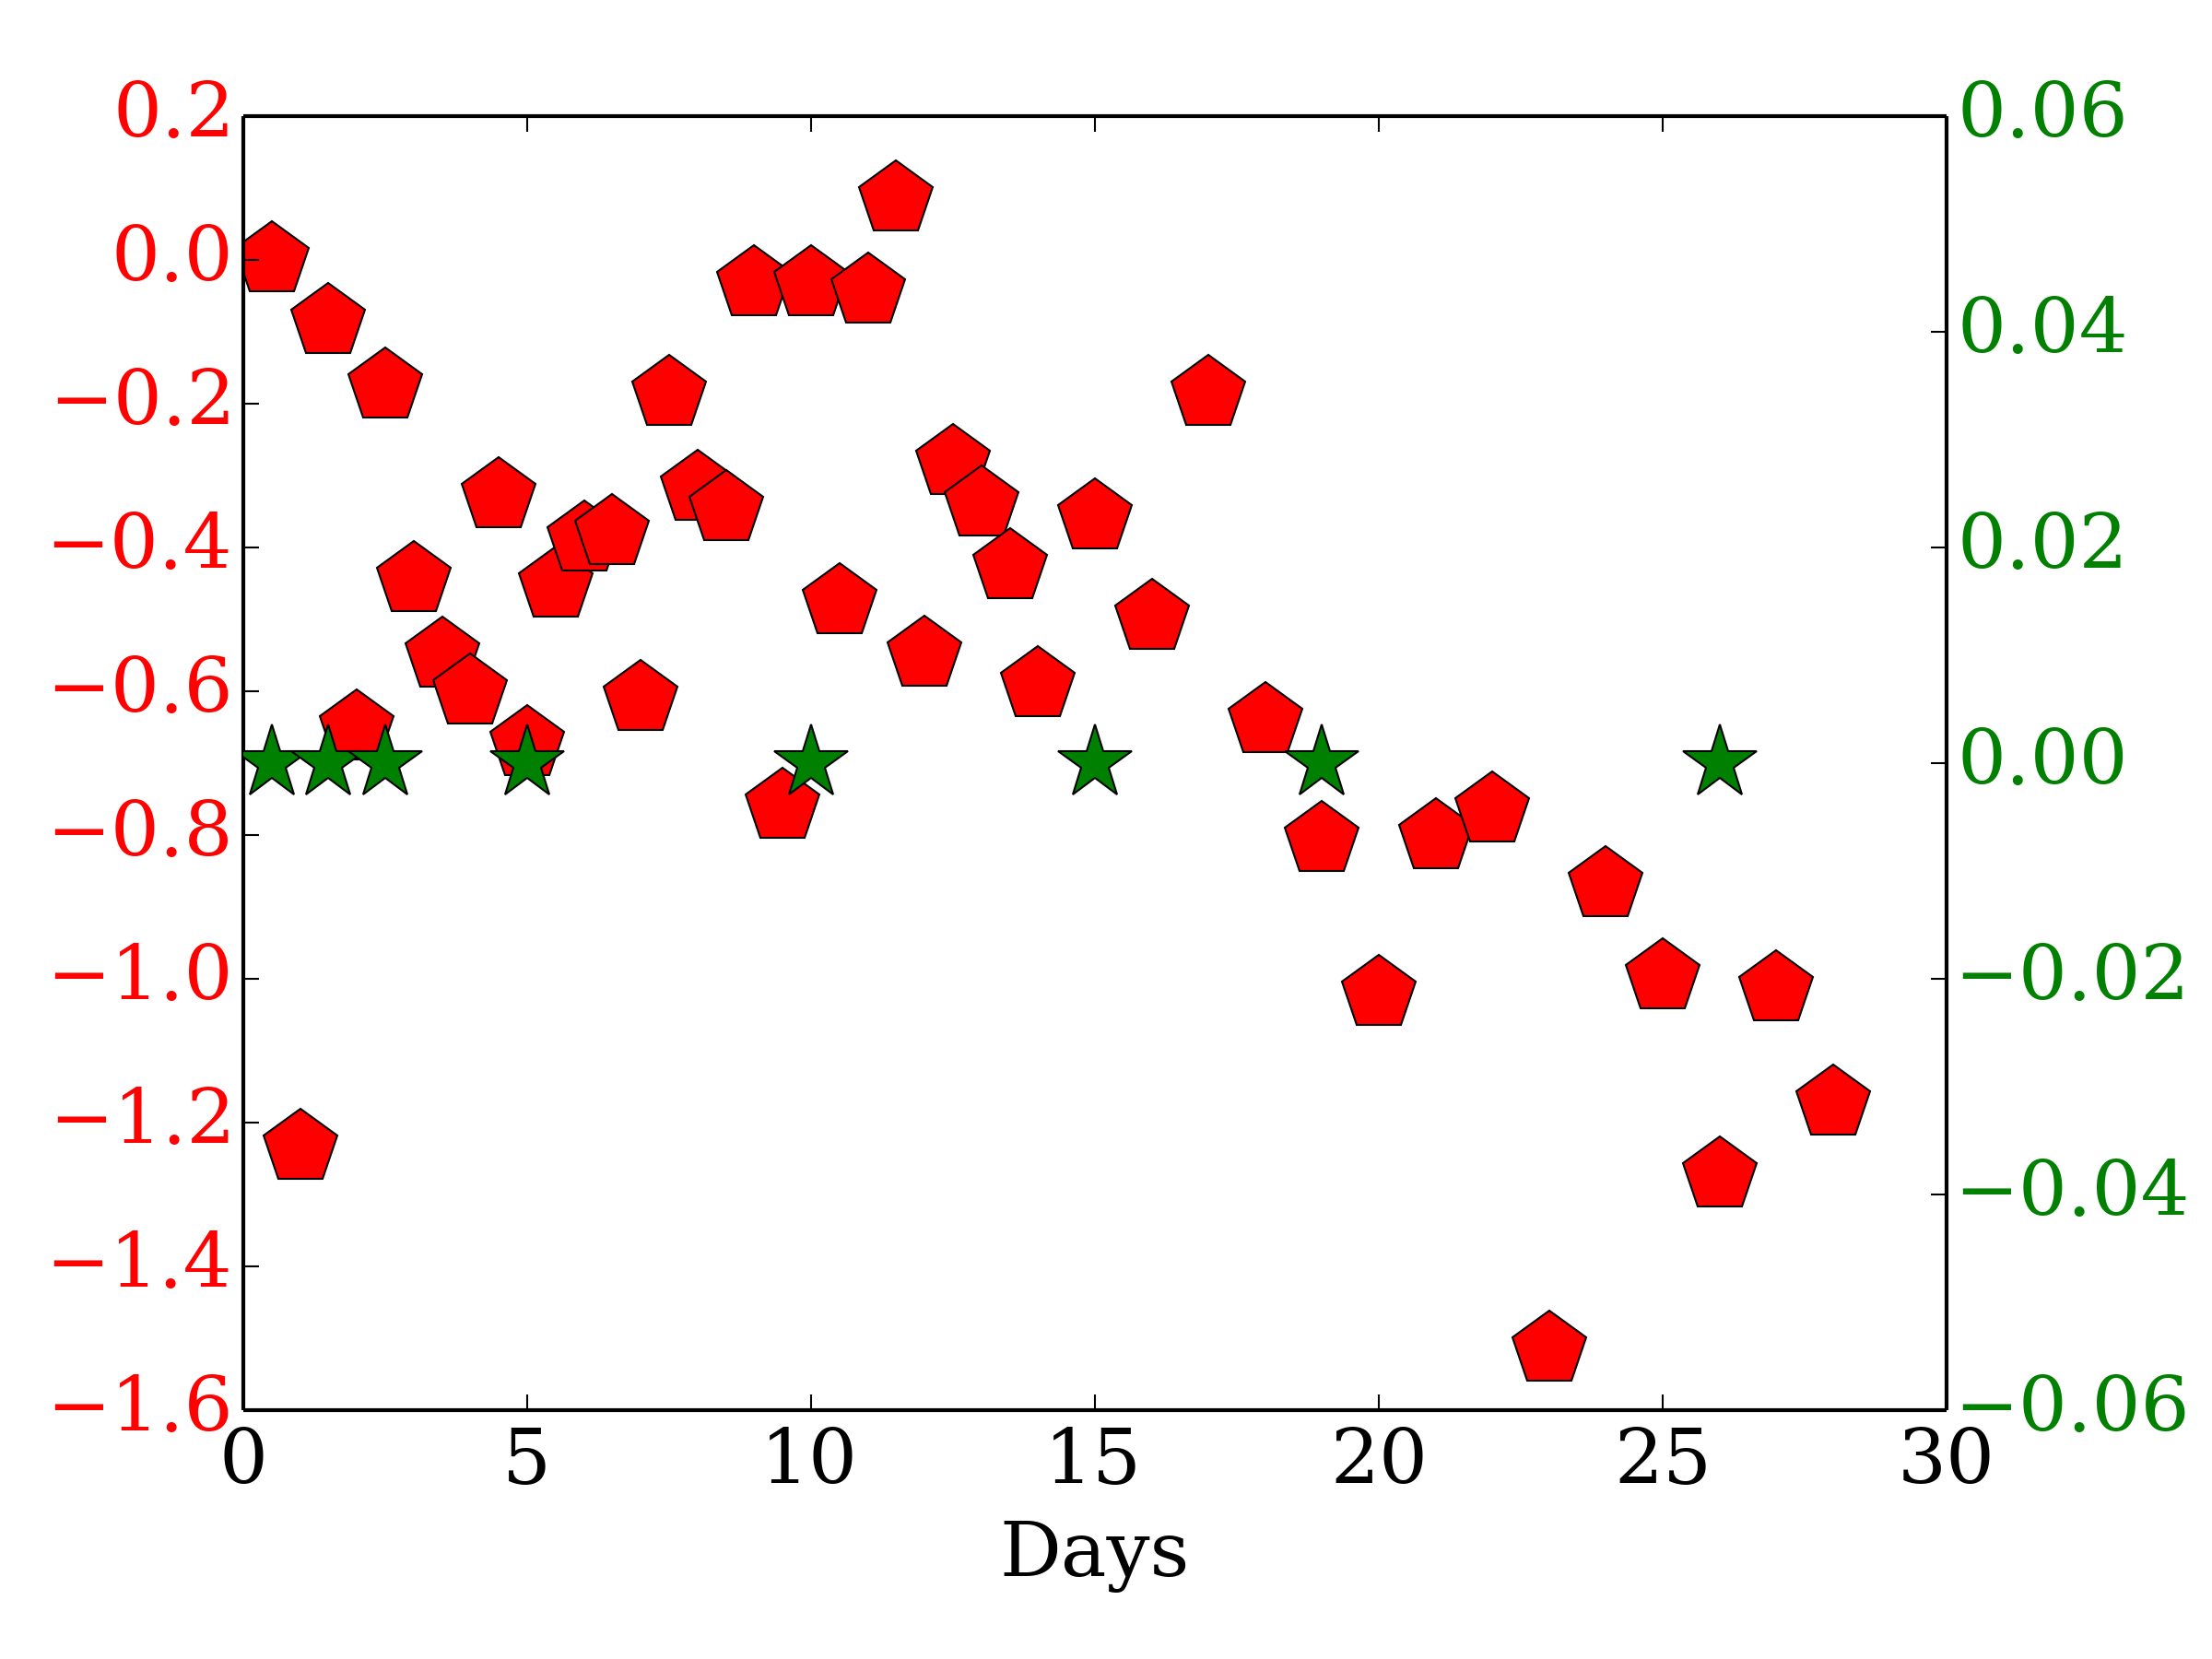
\includegraphics[scale=0.19]{{plots/meth/jointfigures_best/dnmt3a}.png}}
\hfill
\subfloat[SRC]{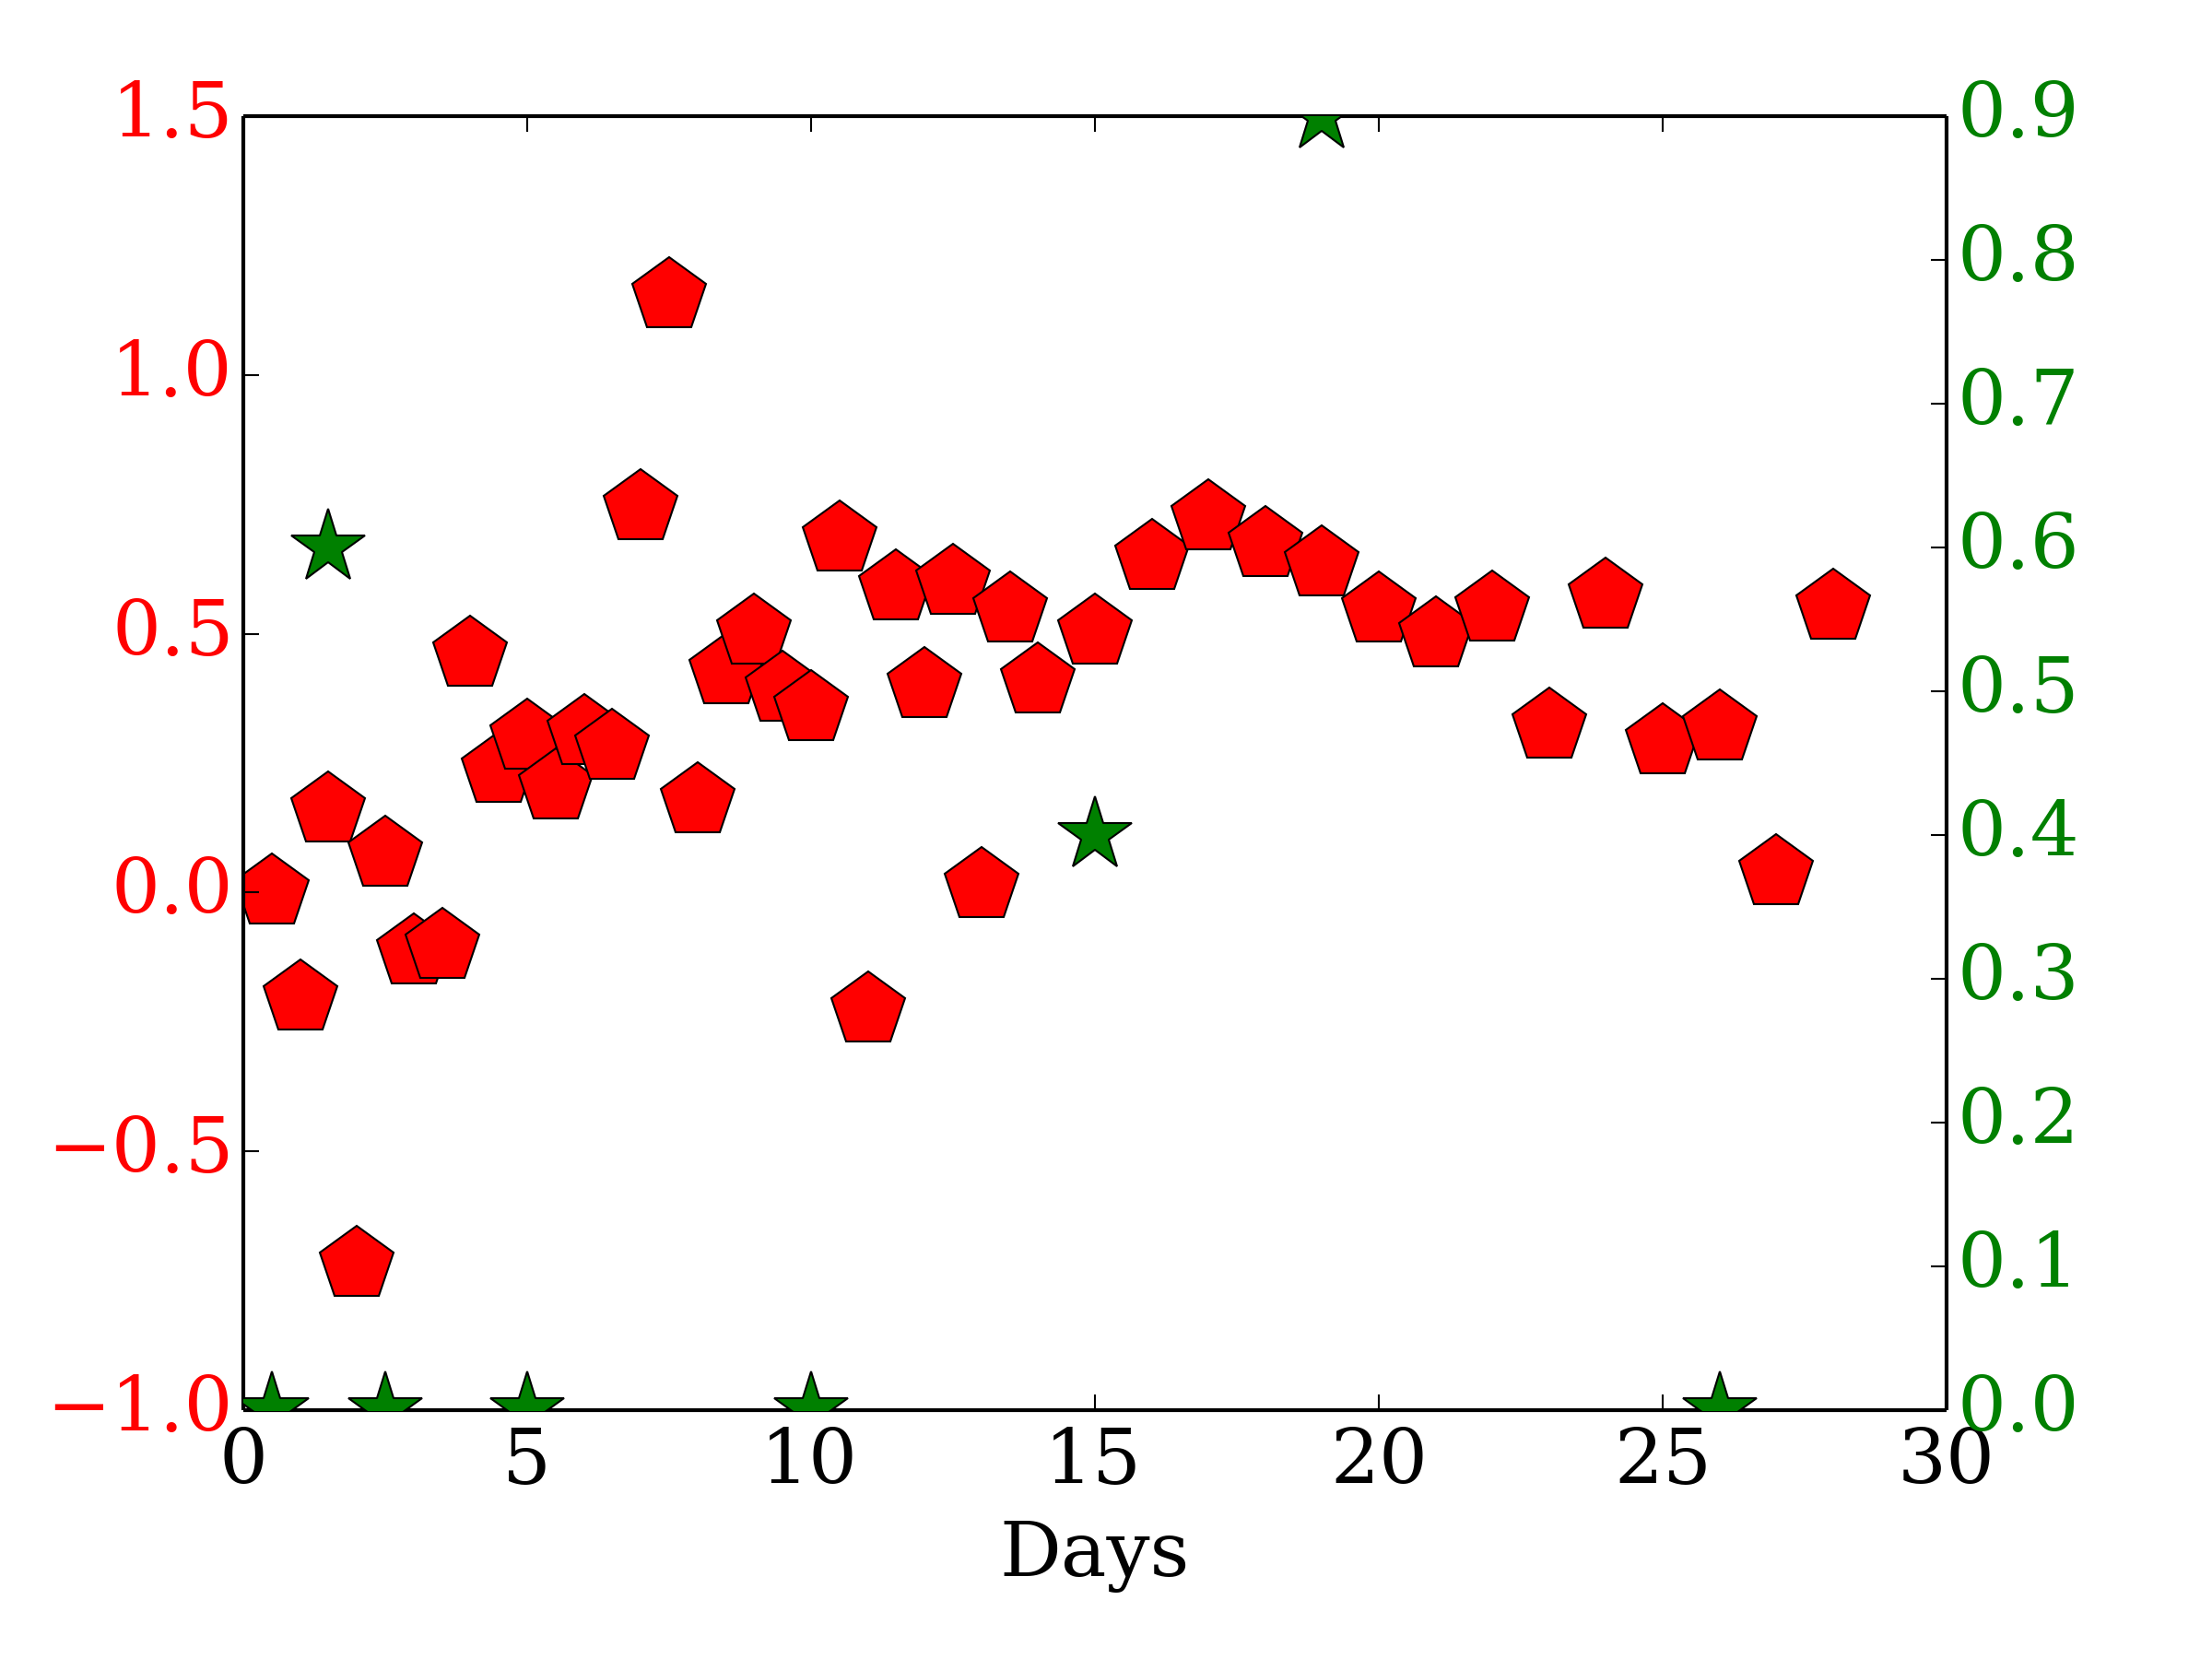
\includegraphics[scale=0.19]{{plots/meth/jointfigures_best/src}.png}}
\hfill
\subfloat[LOX]{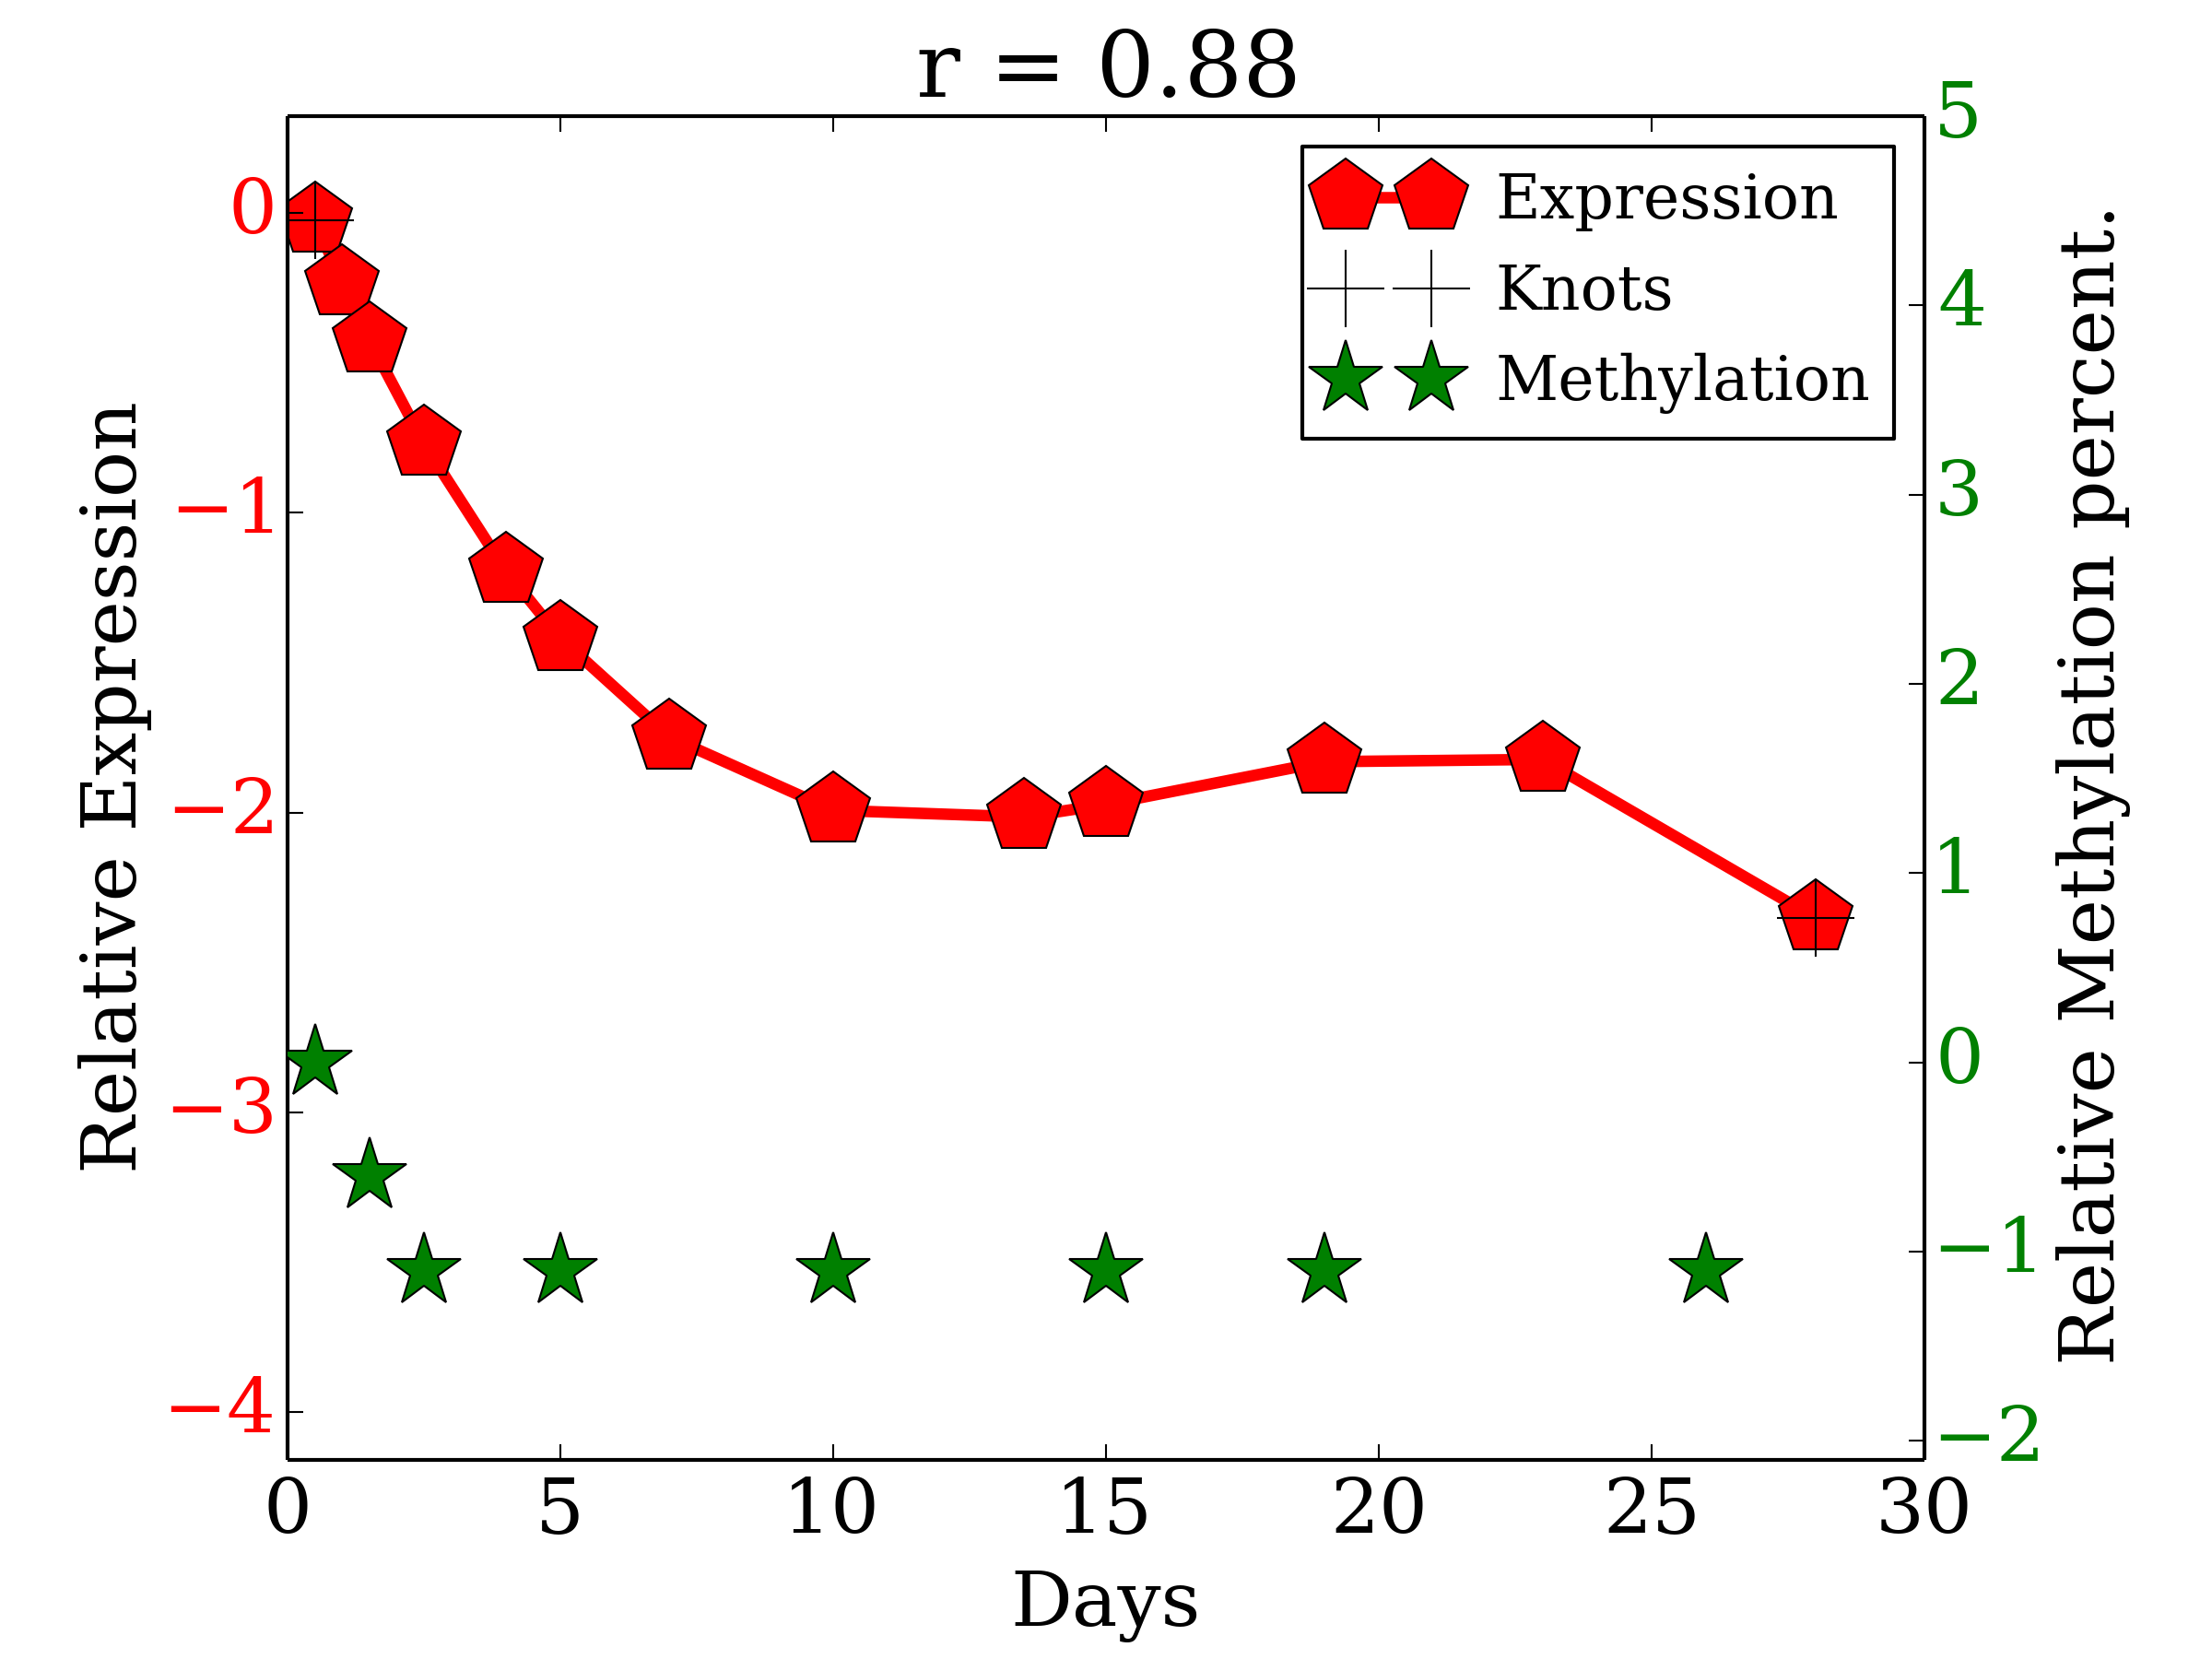
\includegraphics[scale=0.19]{{plots/meth/jointfigures_best/lox}.png}}
\end{minipage}
\caption{Comparison of gene expression and methylation data for genes a) DNMT3A, b) SRC, c) LOX.}
\label{fig:methgene}
\end{figure}


\section{Conclusion}

We develop a method \Tempselect to efficiently identify subset of important
time points over densely sampled gene expression profiles. We show
that these points can be used as candidates for high-throughput profiling
experiments as well as other temporal experiments such as
methylation. Additionally, identified points can serve as a proven
benchmark to reduce the experimental cost.

\bibliographystyle{plain}
\bibliography{expressbib}

\newpage

\appendix


\section{Supplementary Information}


%extra supporting
% We find that best informed guess is to initialize using points that are sorted by increasing absolute
% differences. Using additional anchor points such as E16.5 and E18.5
% for analyses leads to similar results. We also enumerated top $10$ optimal solutions by running \Tempselect
% across many initial conditions. We find selected points and errors of
% these solutions to be quite similar to our solution above~(See
% Supplementary Table~\ref{tab:xxx}). This trend is also observed when
% we select fewer points, we find similar results when we enumerate all
% possible solutions of size $6$ to examine the optimality structure of the solution space. 

\setcounter{figure}{0}   
\begin{figure}[ht]
\centering
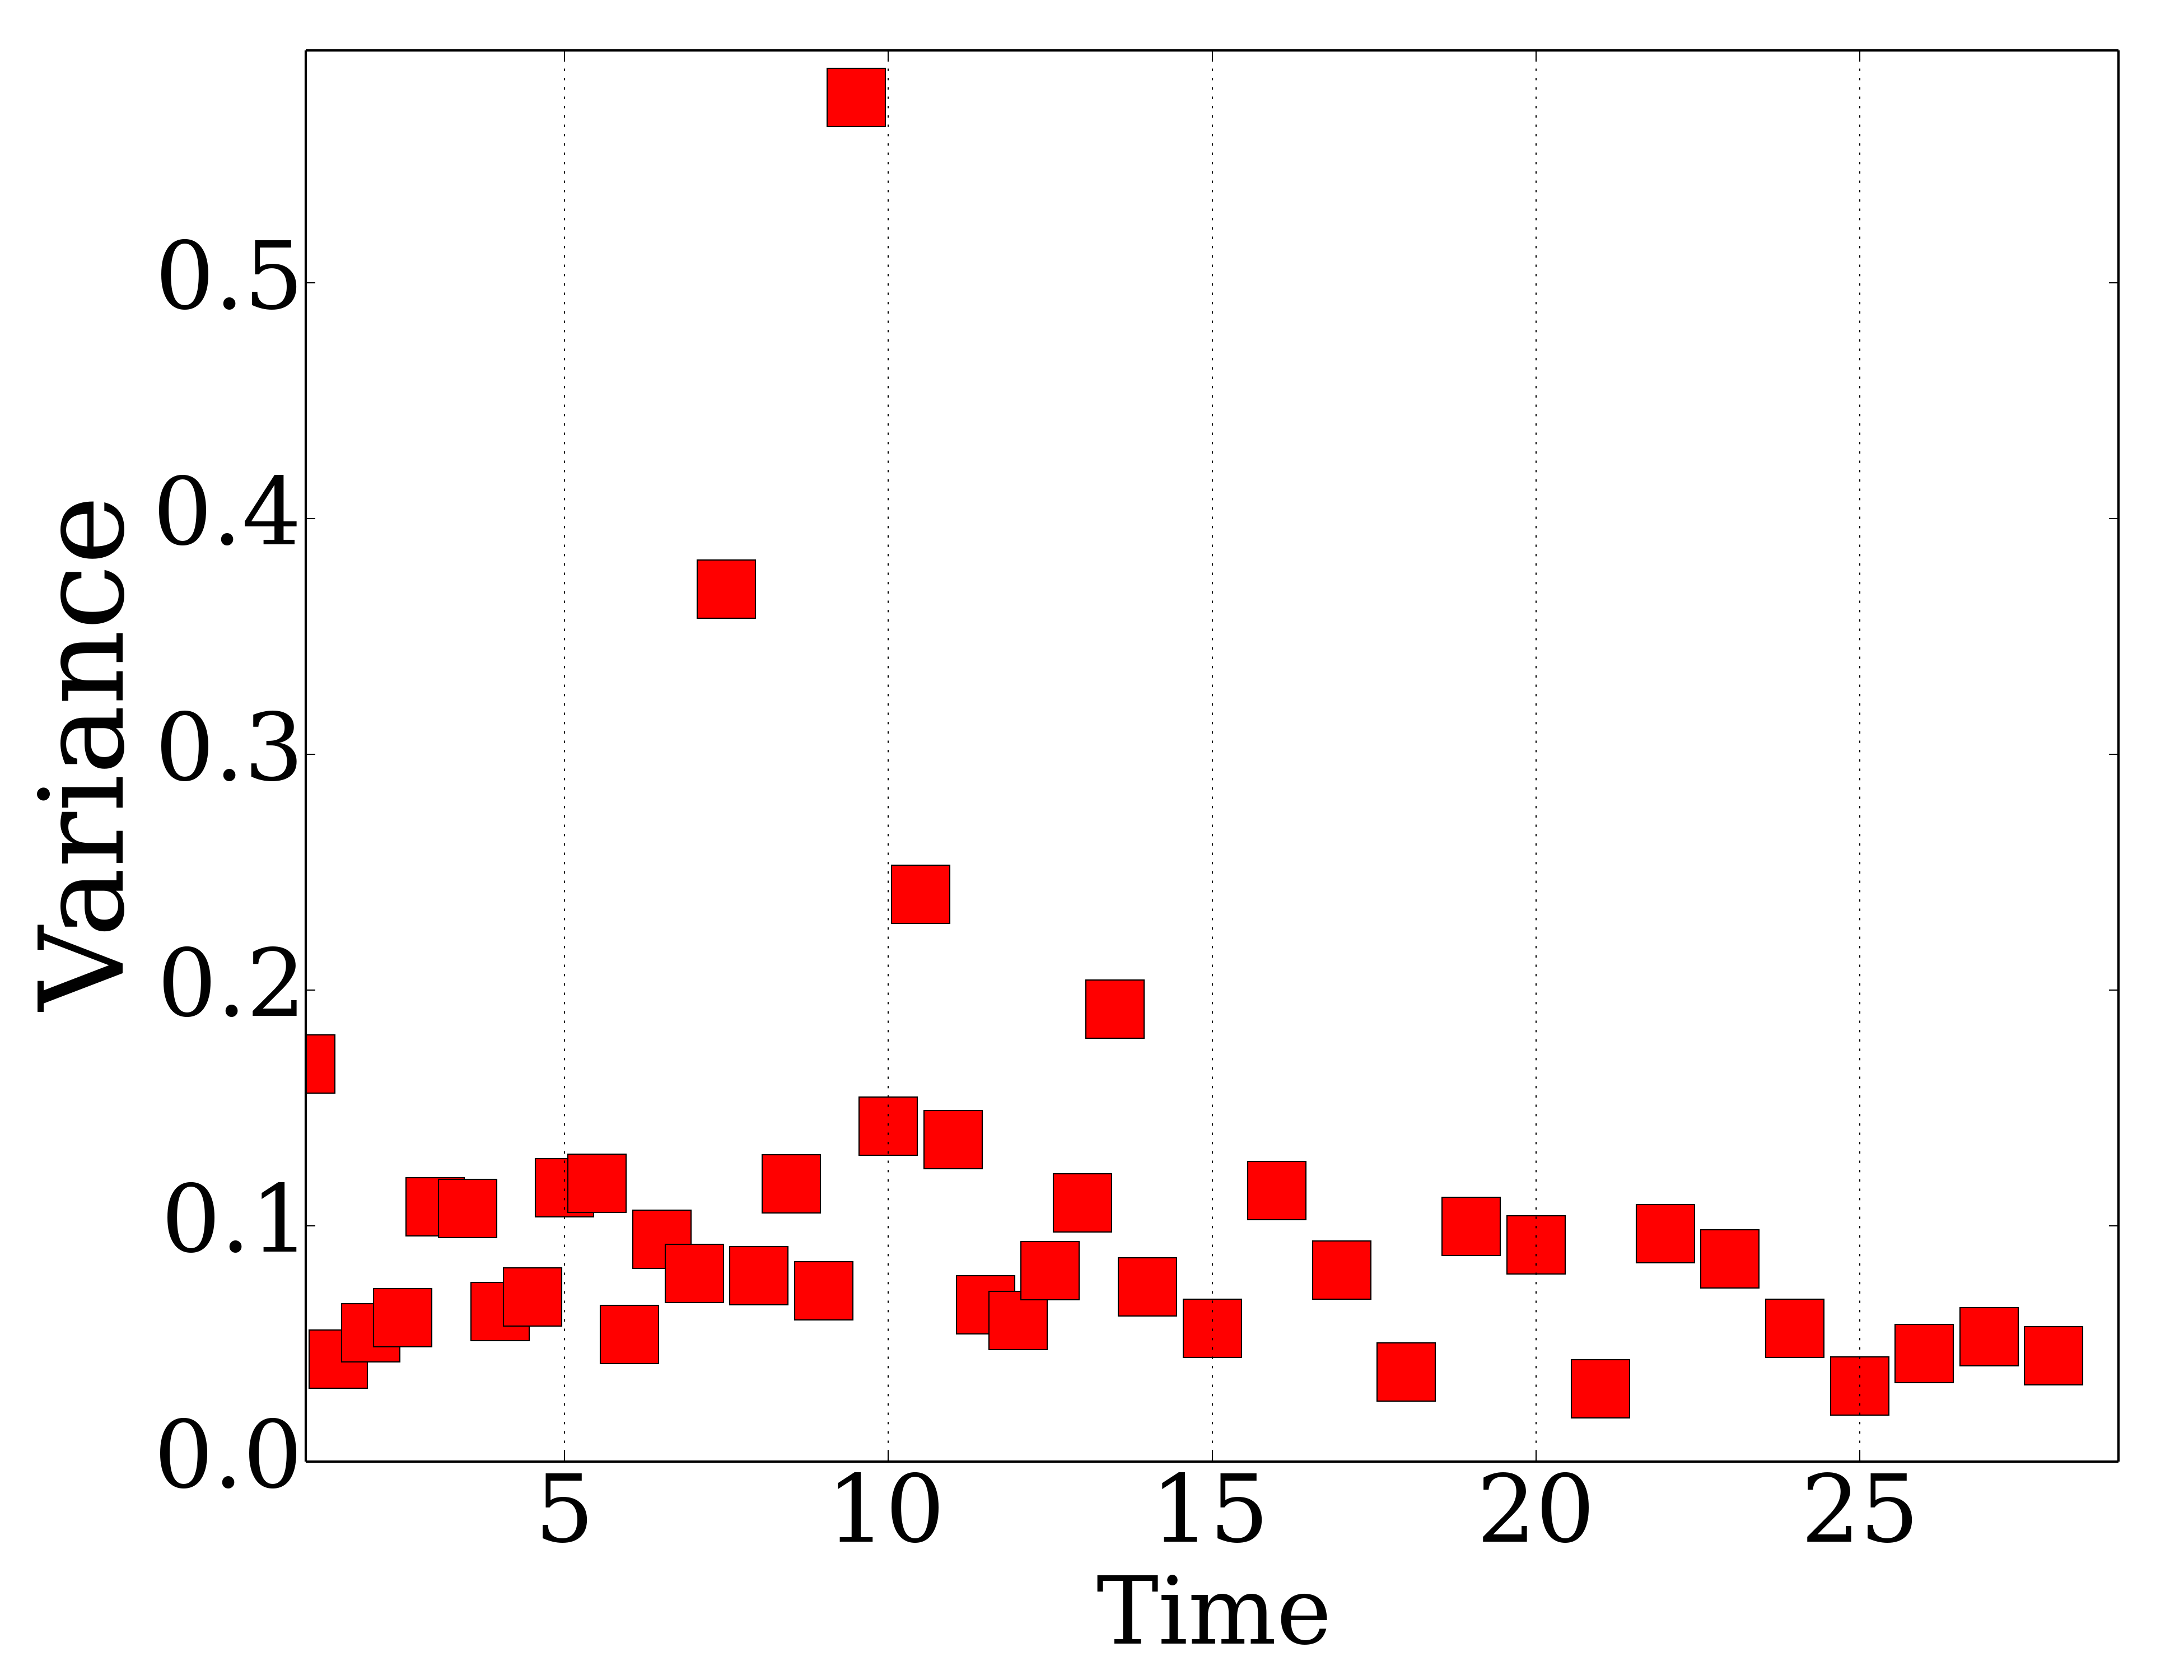
\includegraphics[scale=0.2]{{plots/newdata/timeerror}.png}
\caption{Average noise in each time point}
\label{fig:sup1}
\end{figure}

\begin{figure}
\centering
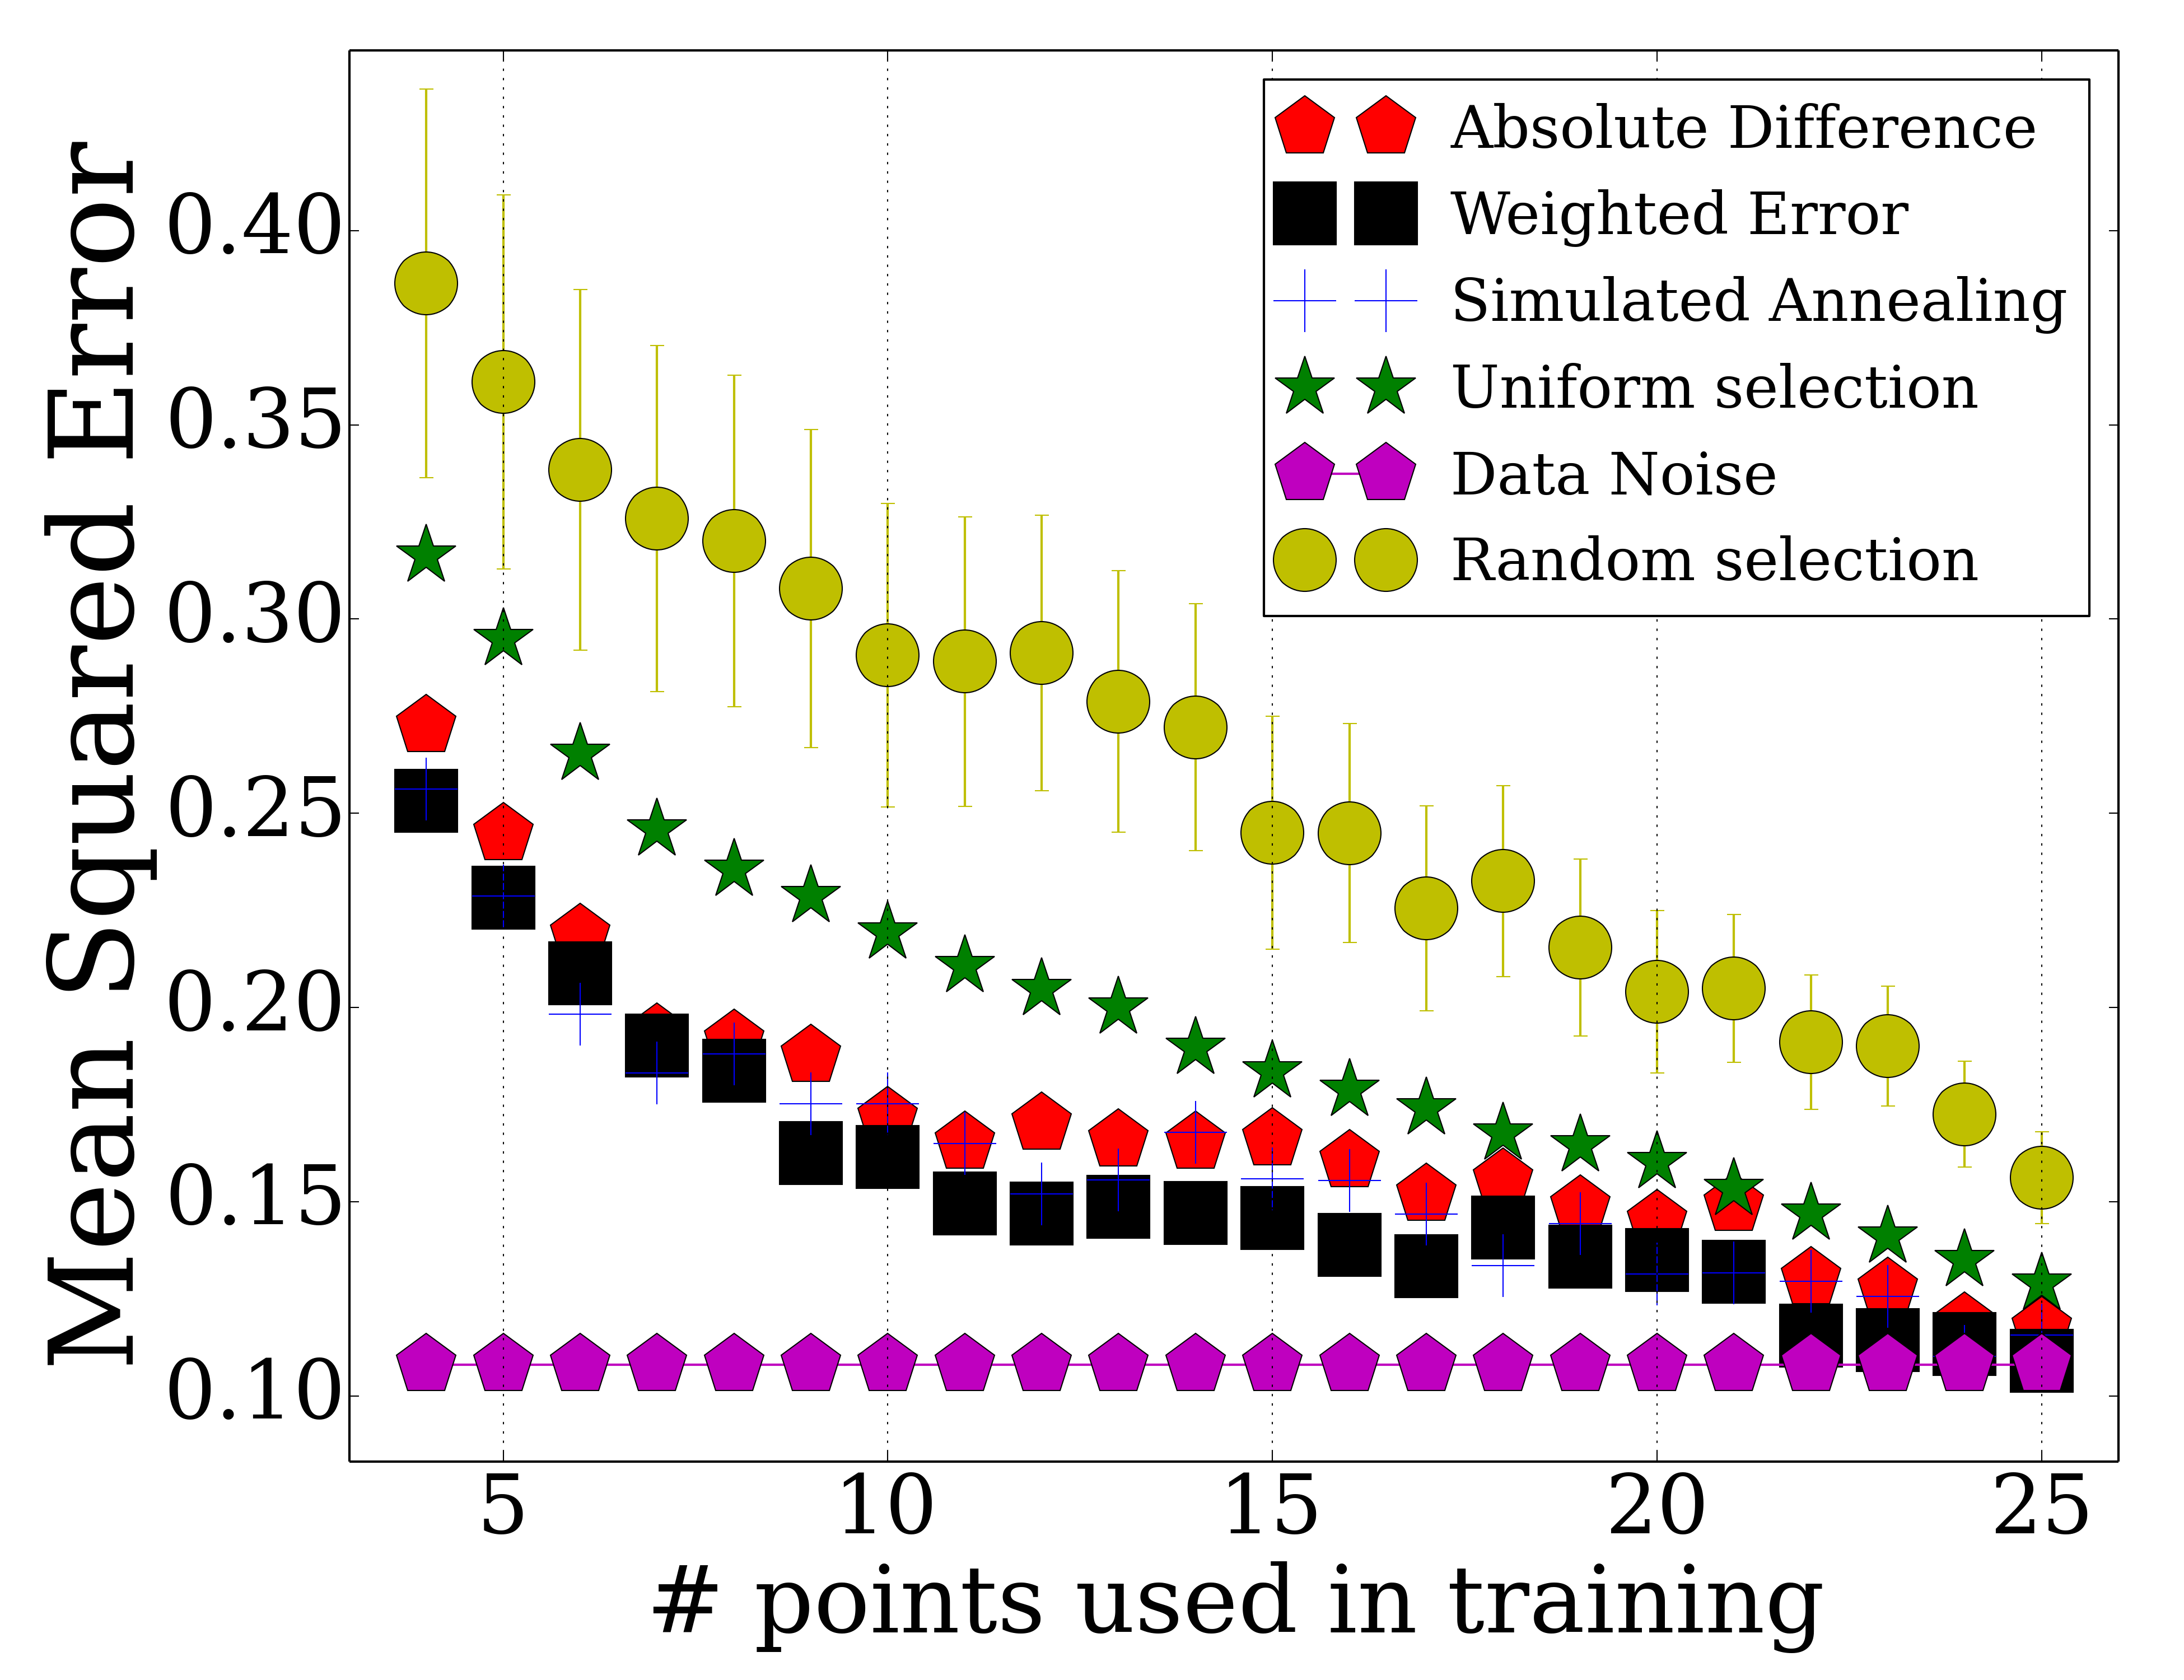
\includegraphics[scale=0.2]{{plots/newdata/performRL2}.png}
\caption{Performance of \Tempselect by increasing number of selected points}
\label{fig:sup2}
\end{figure}

\begin{figure}
\begin{minipage}{1.0\textwidth}
\subfloat[ERB]{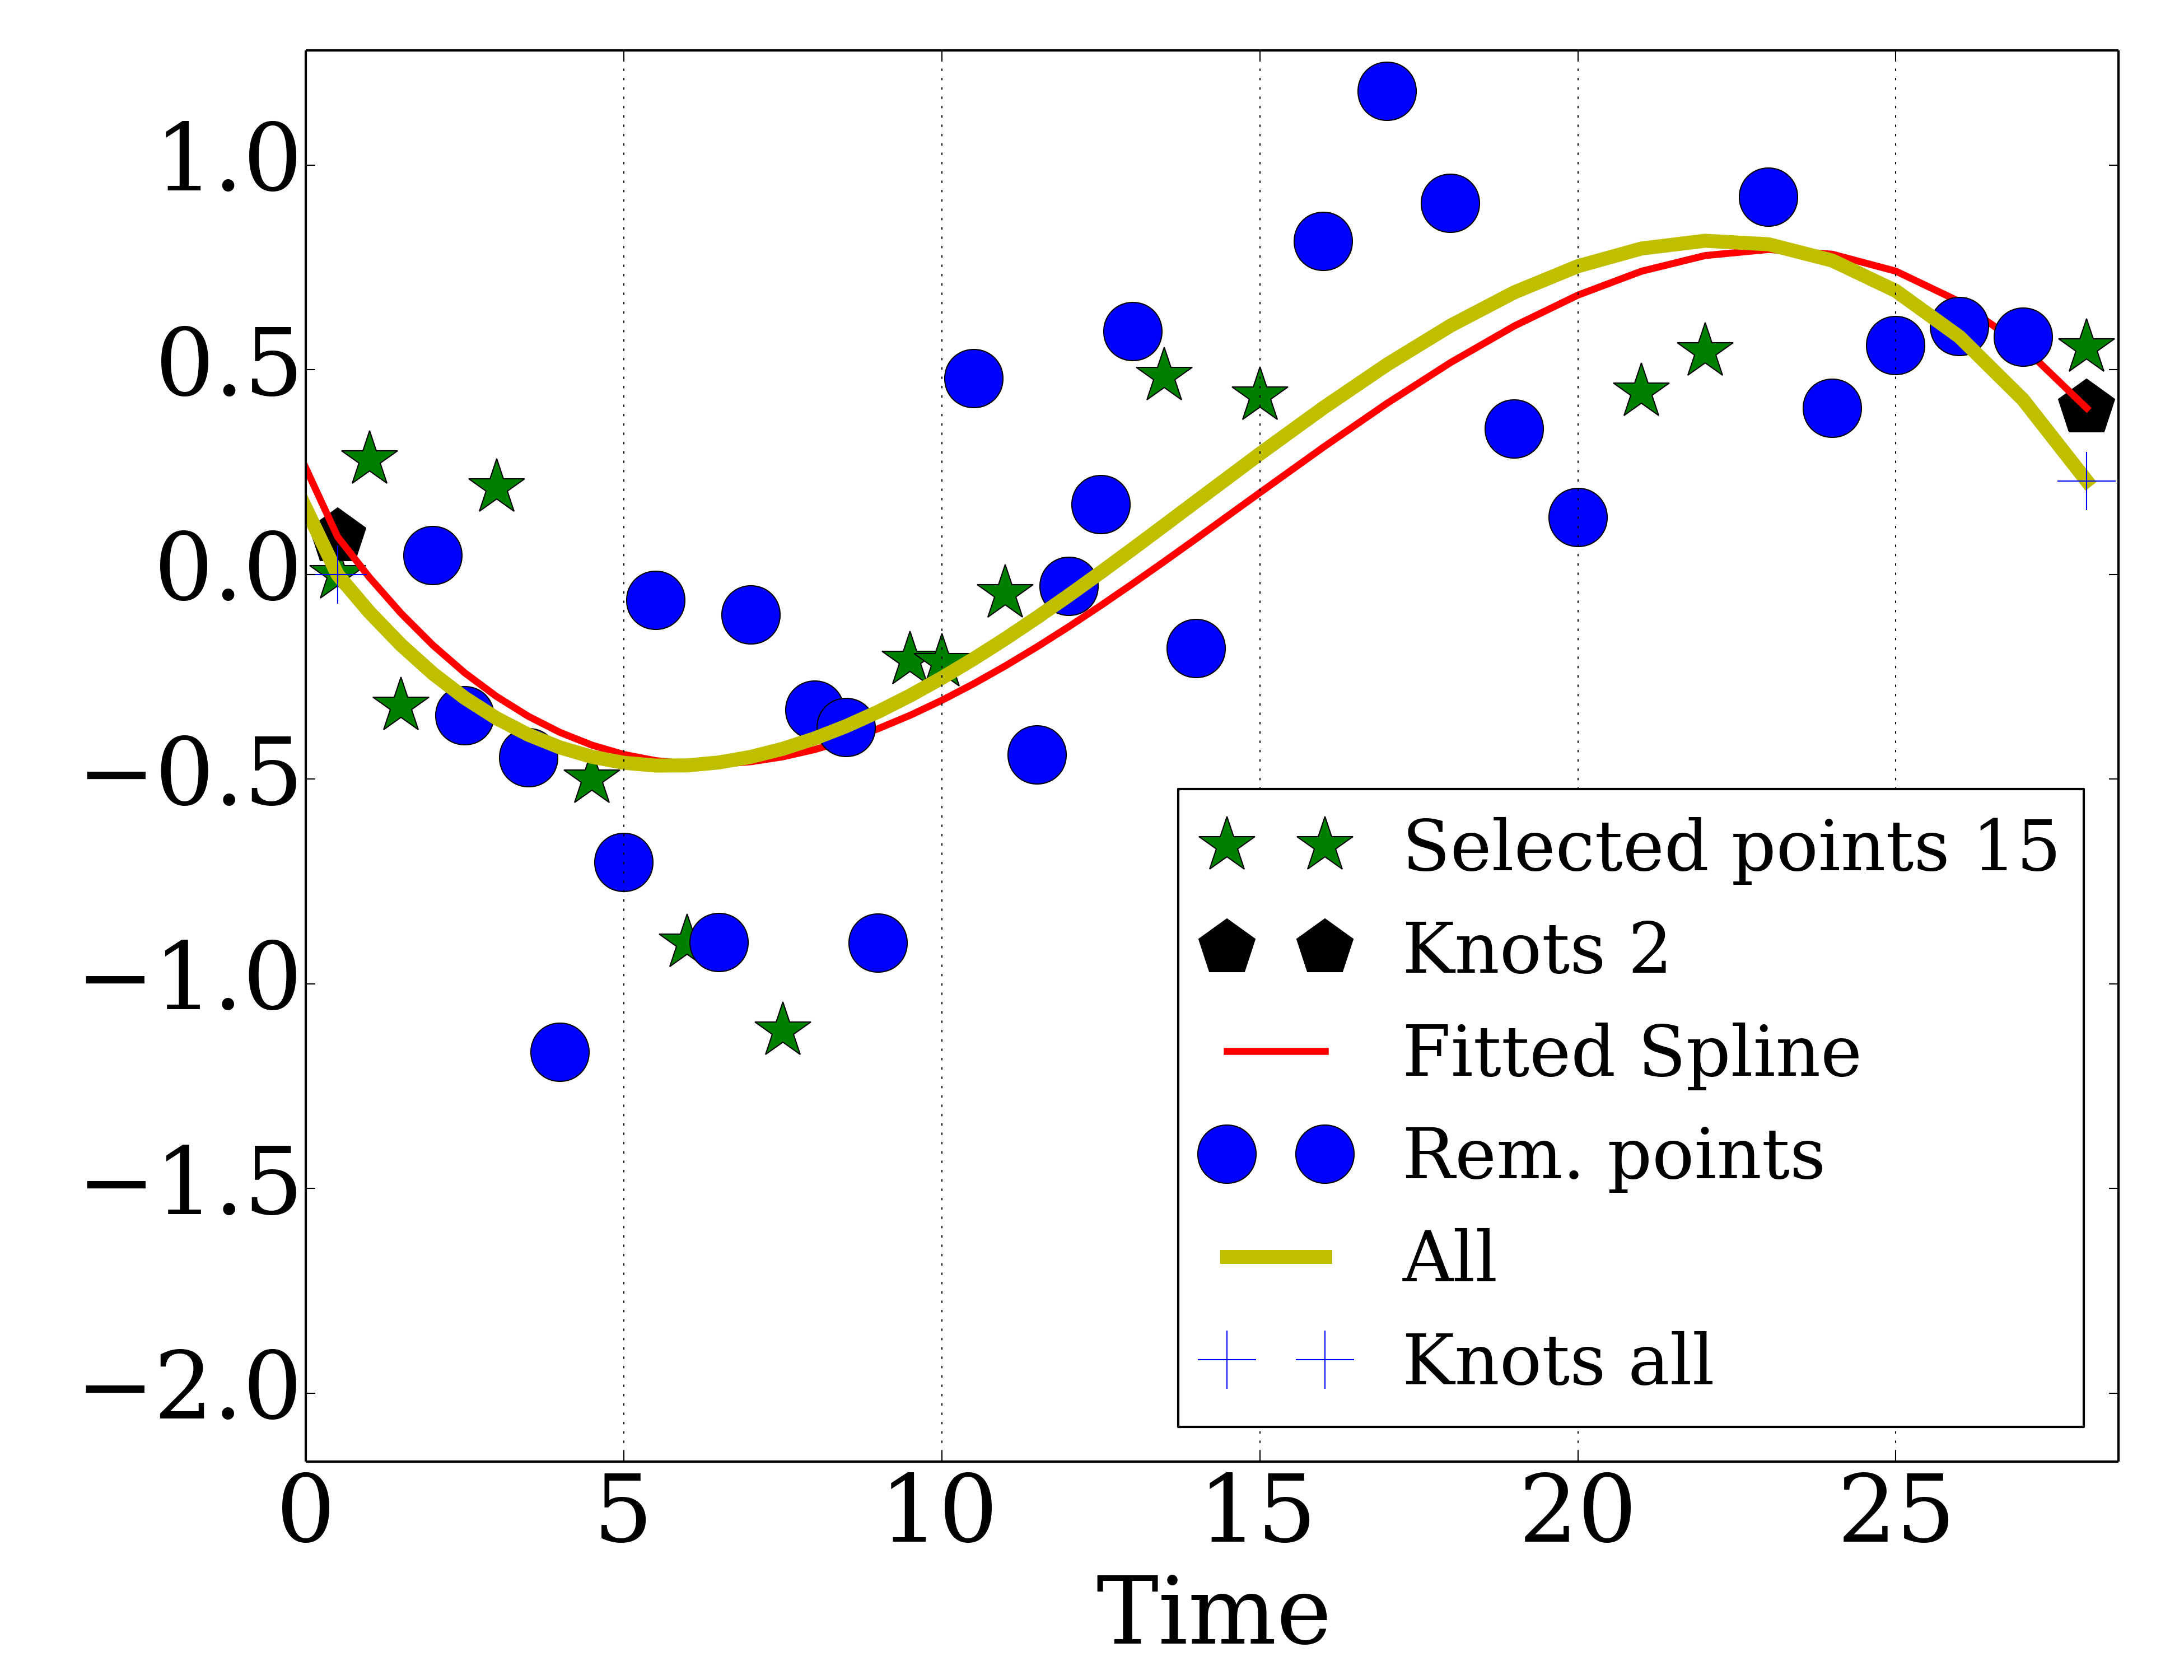
\includegraphics[scale=0.12]{{plots/newdata/splineplots15/ERB_15_all}.png}}
\hfill
\subfloat[NME3]{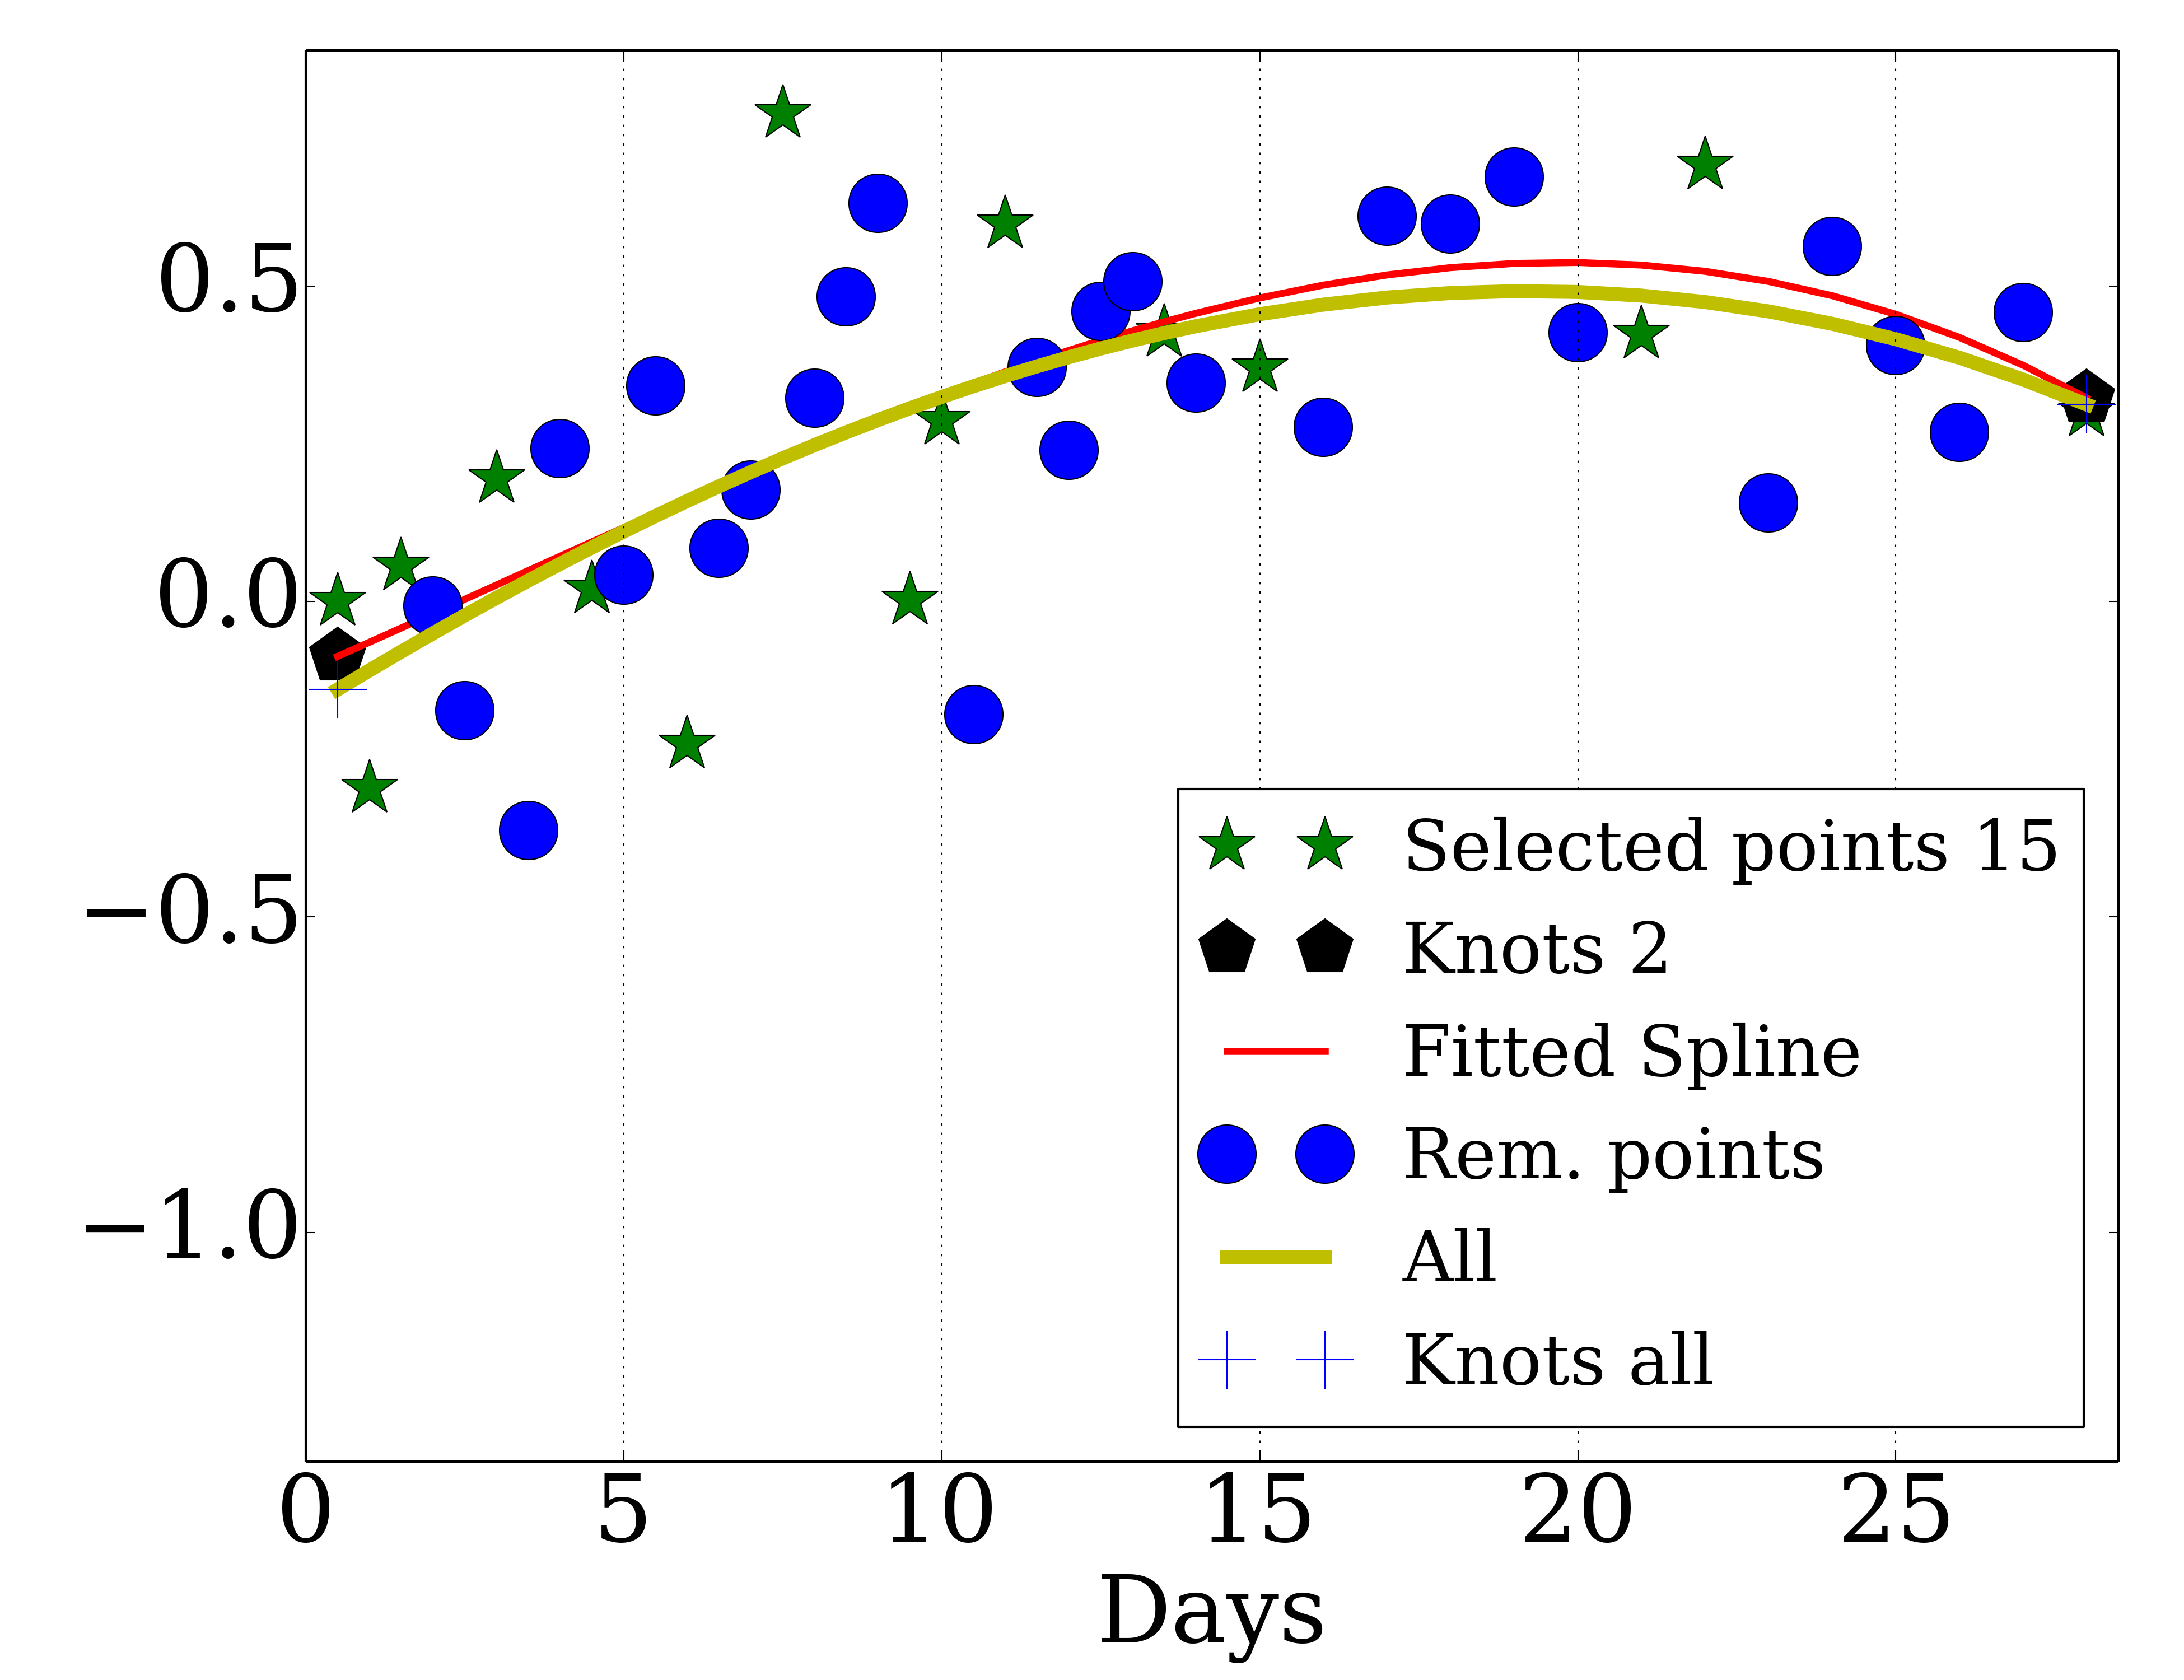
\includegraphics[scale=0.12]{{plots/newdata/splineplots15/NME3_15_all}.png}}
\hfill
\subfloat[POL2RA]{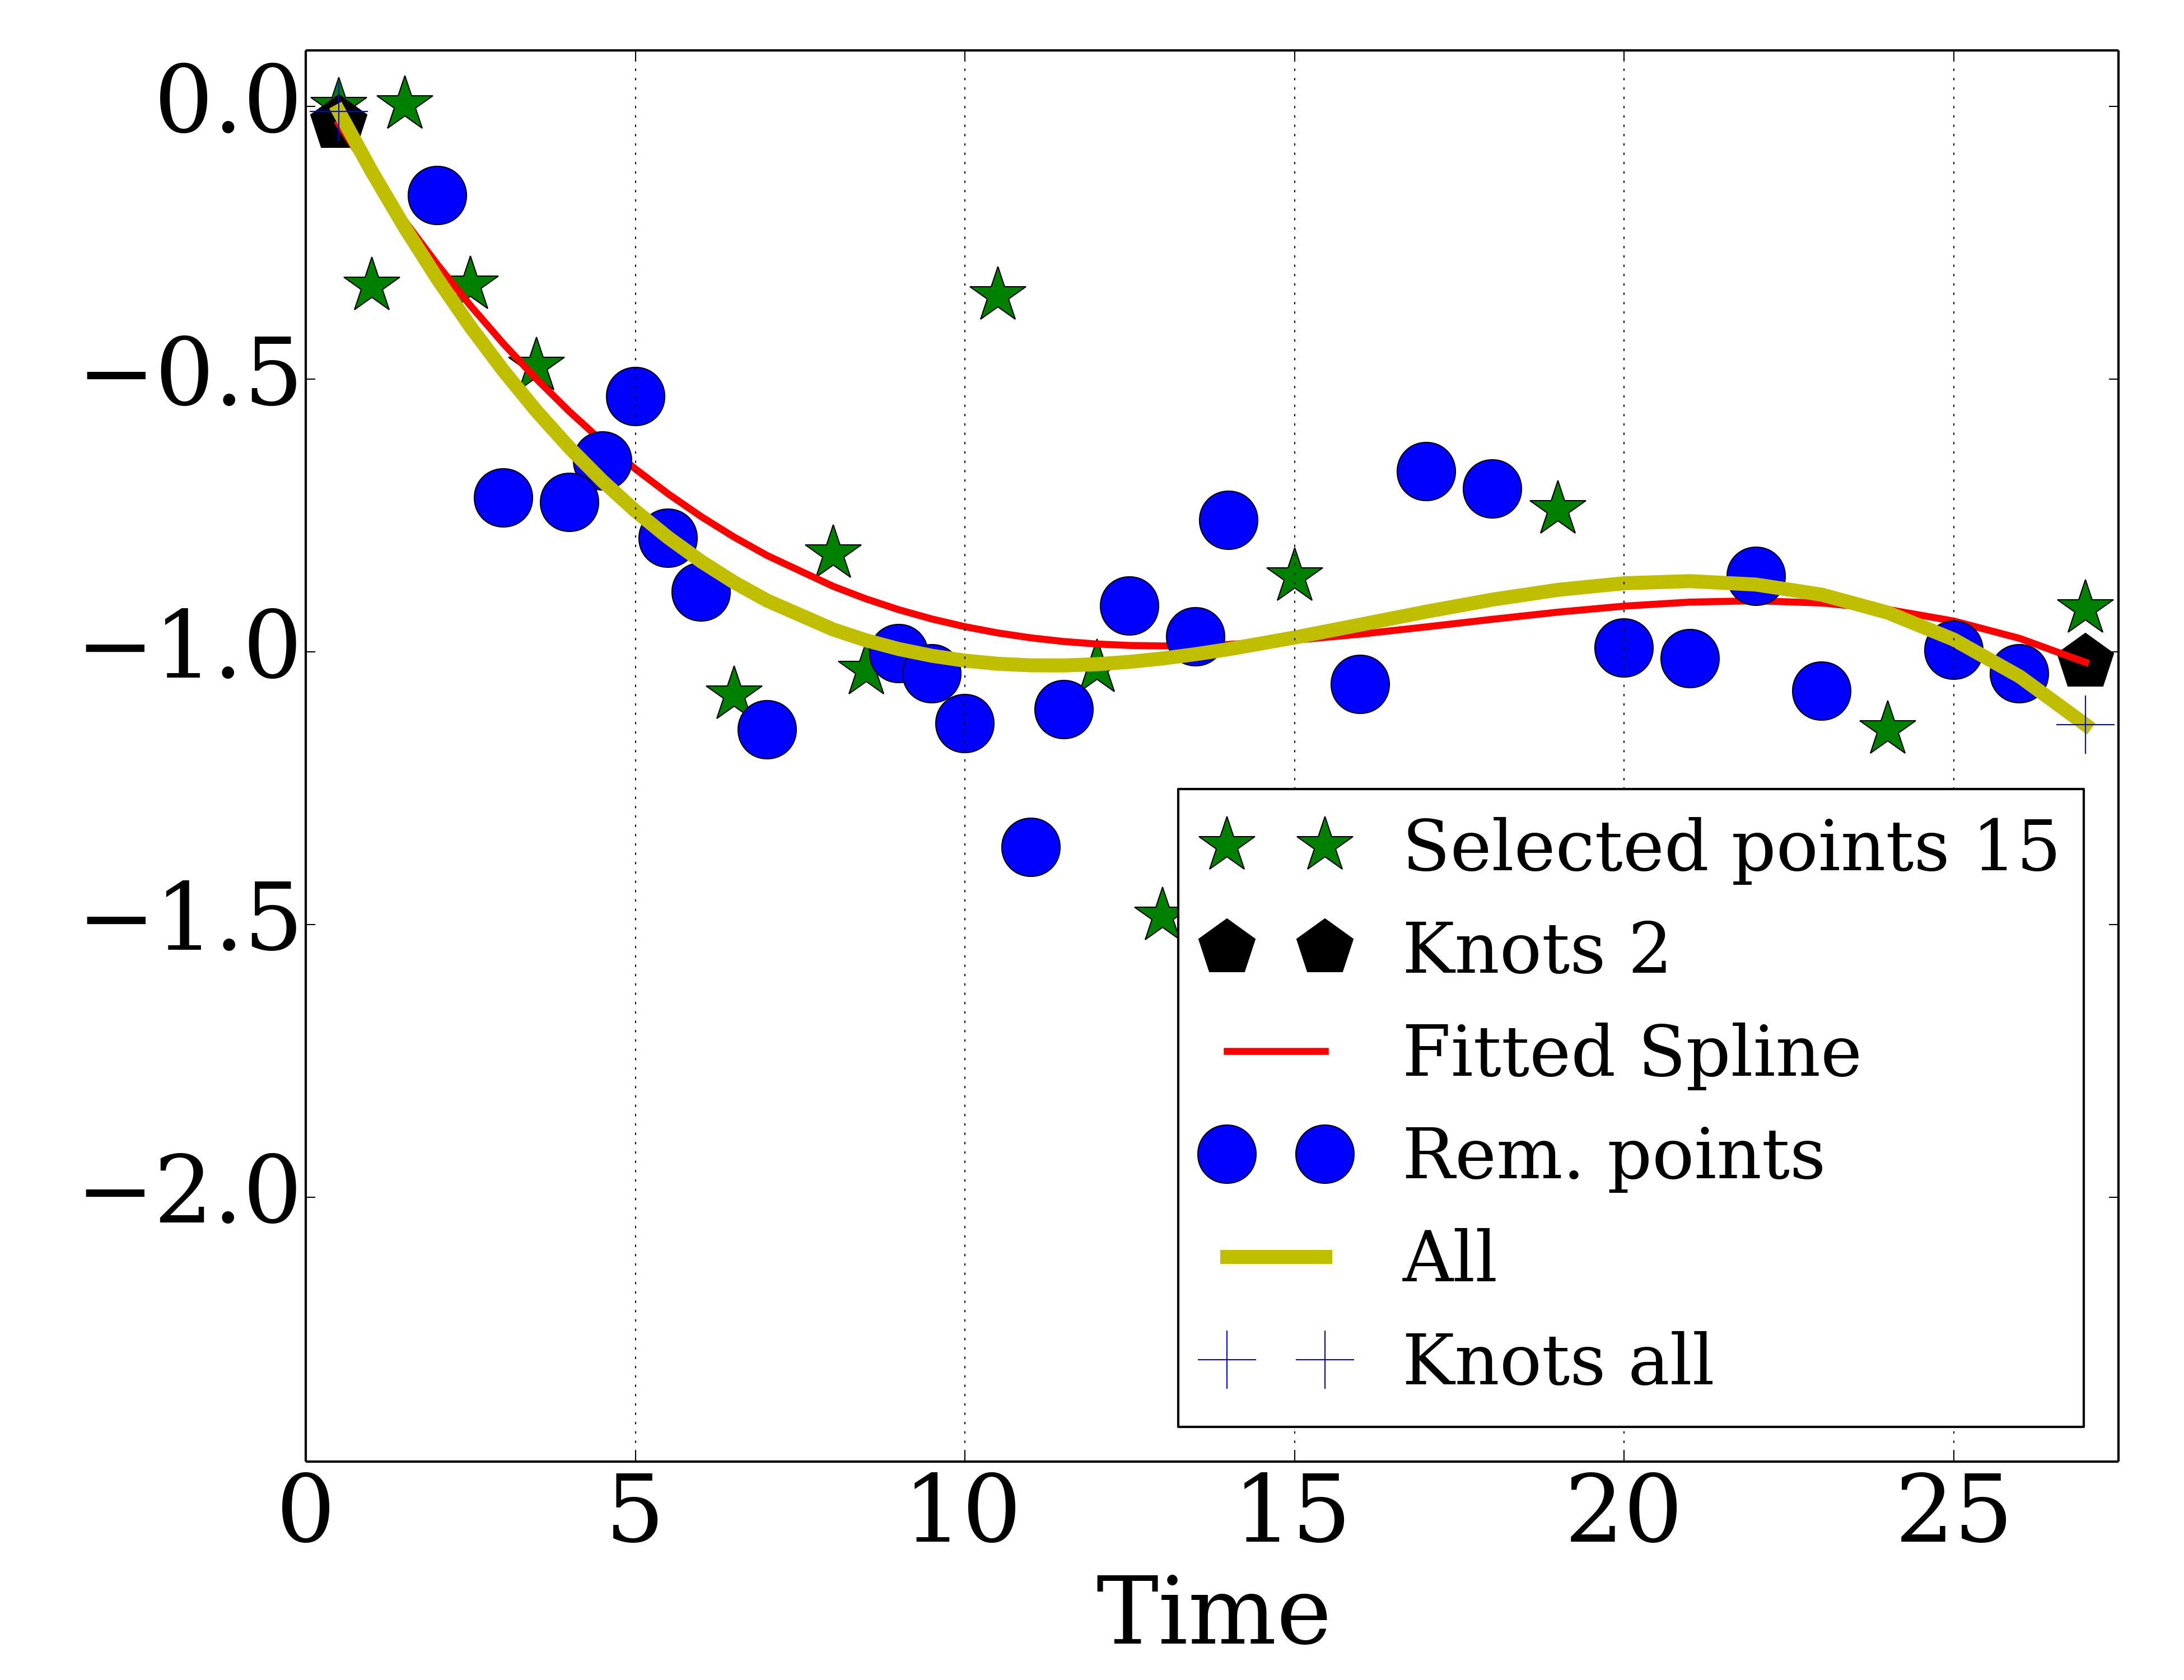
\includegraphics[scale=0.12]{{plots/newdata/splineplots15/polr2a_15_all}.png}}
\hfill
\end{minipage}
\caption{Expression profiles over several genes a) ERB, b) NME3, c) POL2RA}
\label{fig:sup3}
\end{figure}

\begin{figure}
\begin{minipage}{1.0\textwidth}
\subfloat[PDGFRA]{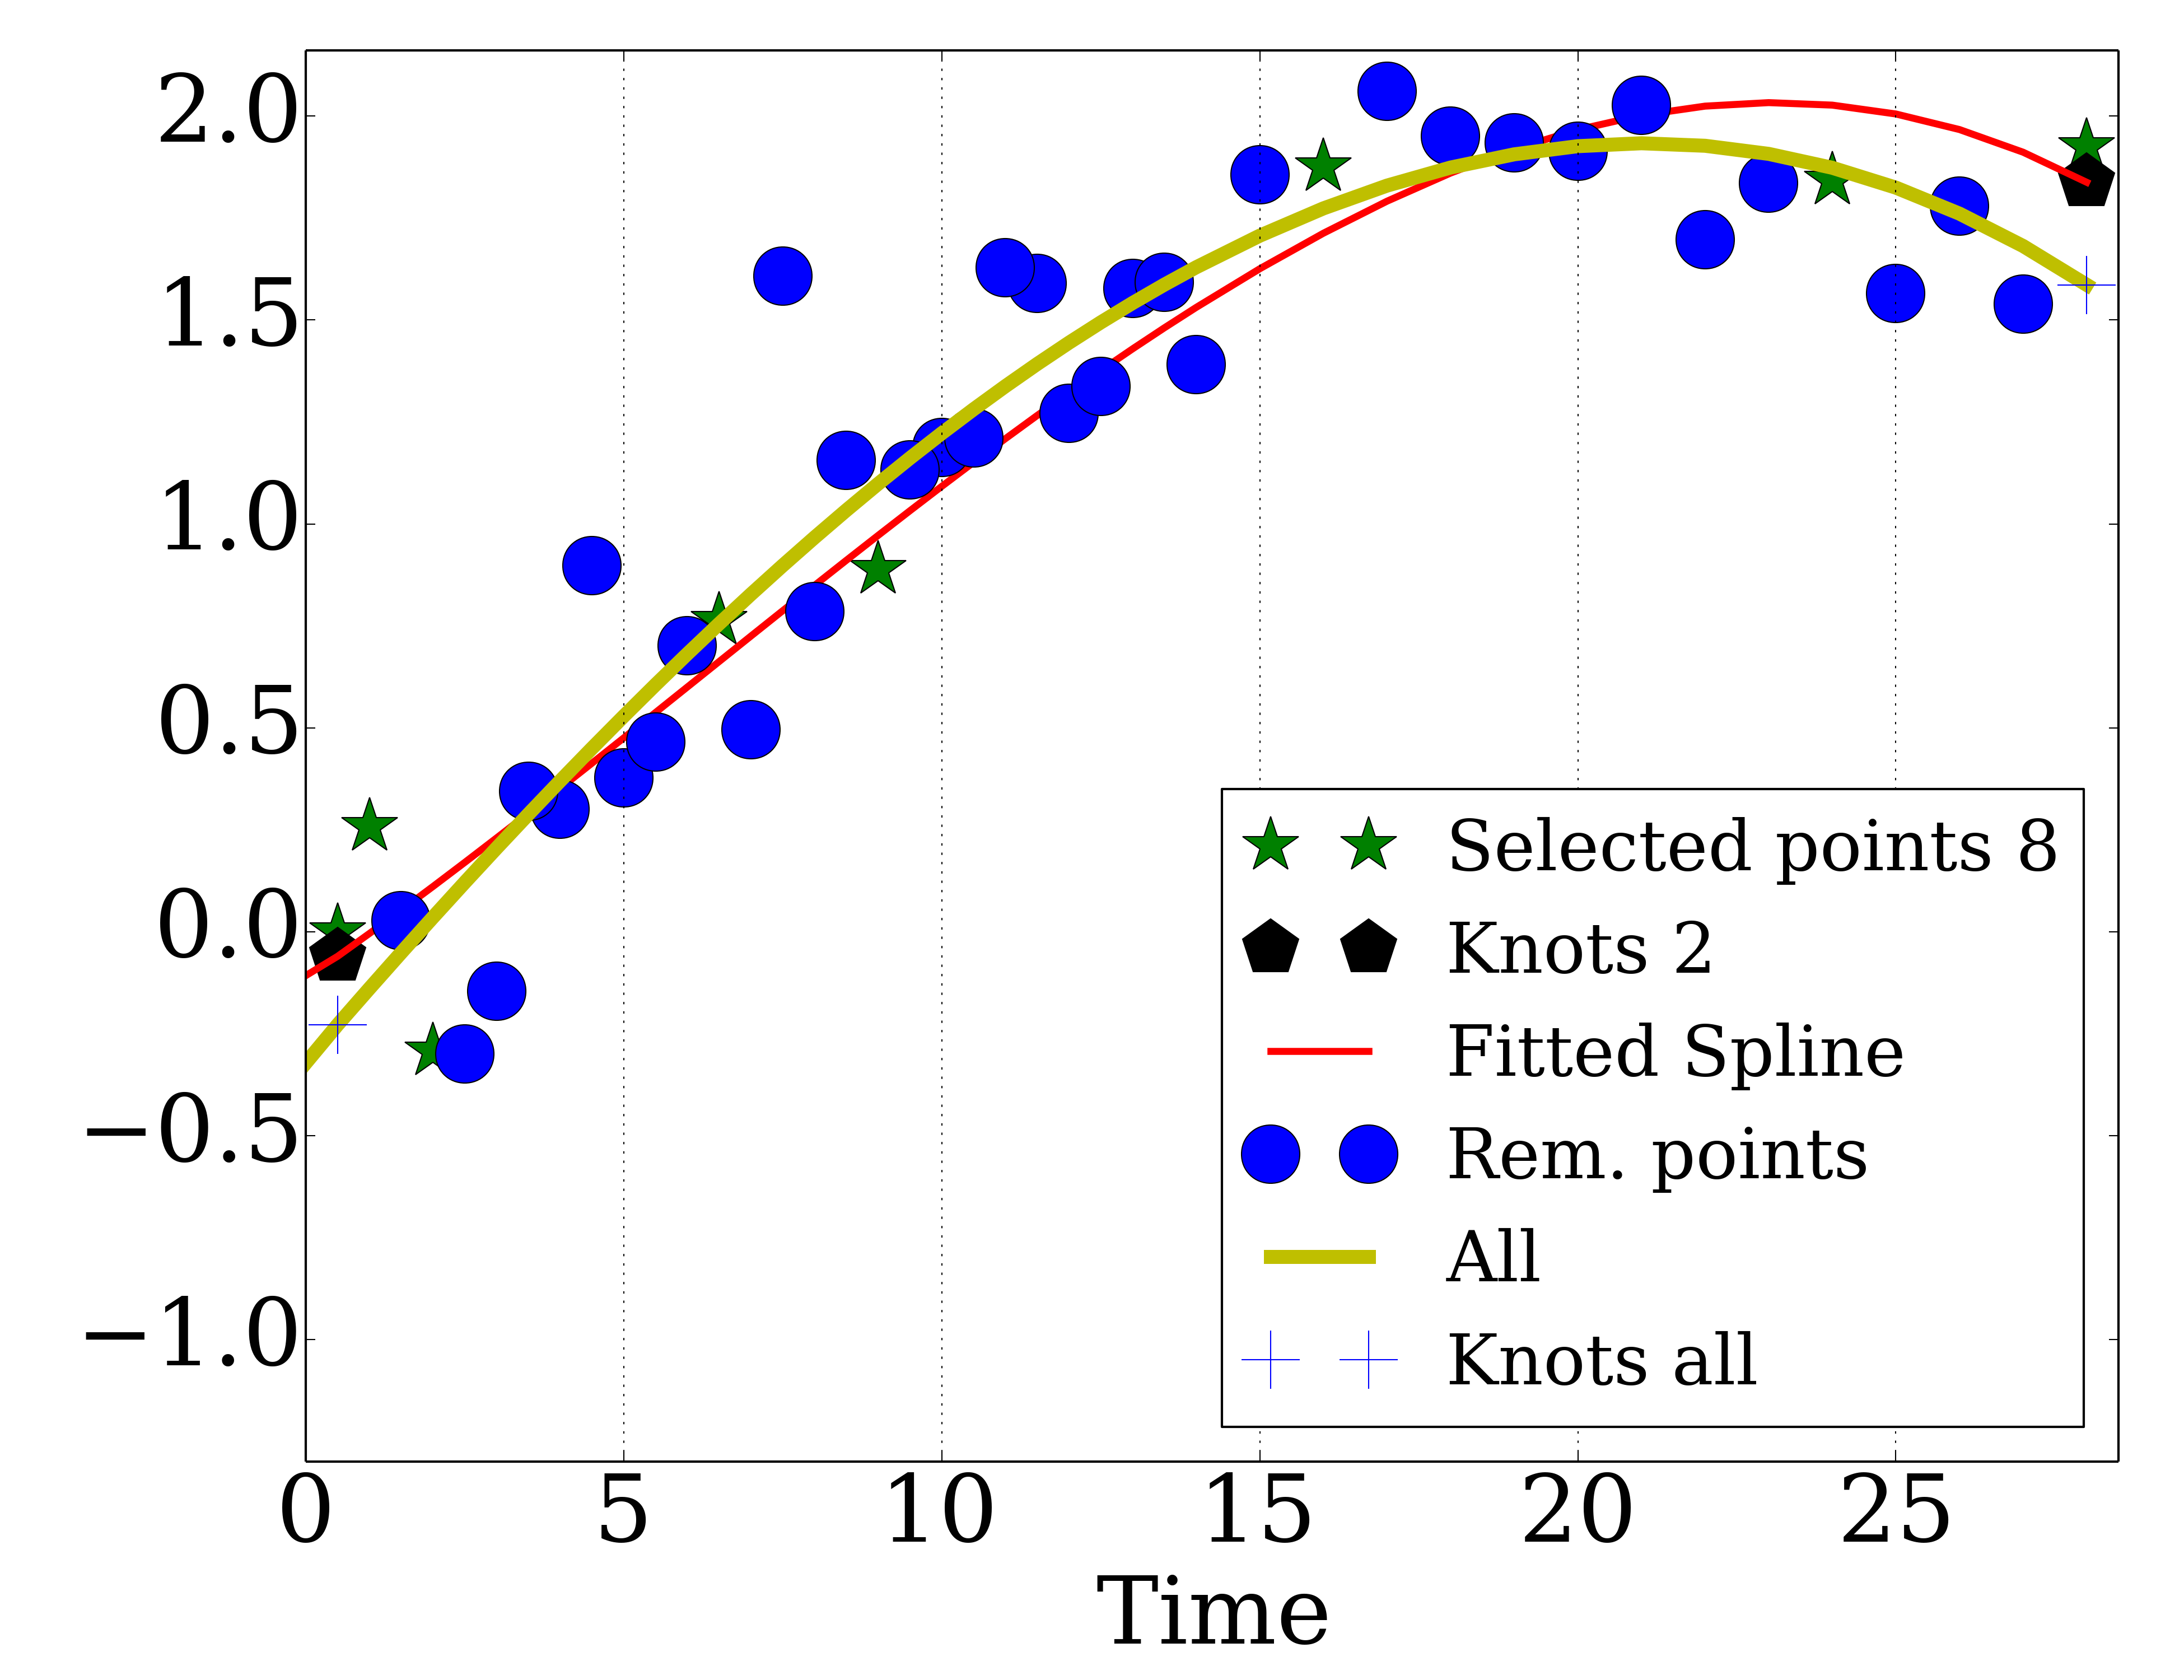
\includegraphics[scale=0.12]{{plots/newdata/splineplots8/PDGFRA_8_all}.png}}
\hfill
\subfloat[ELN]{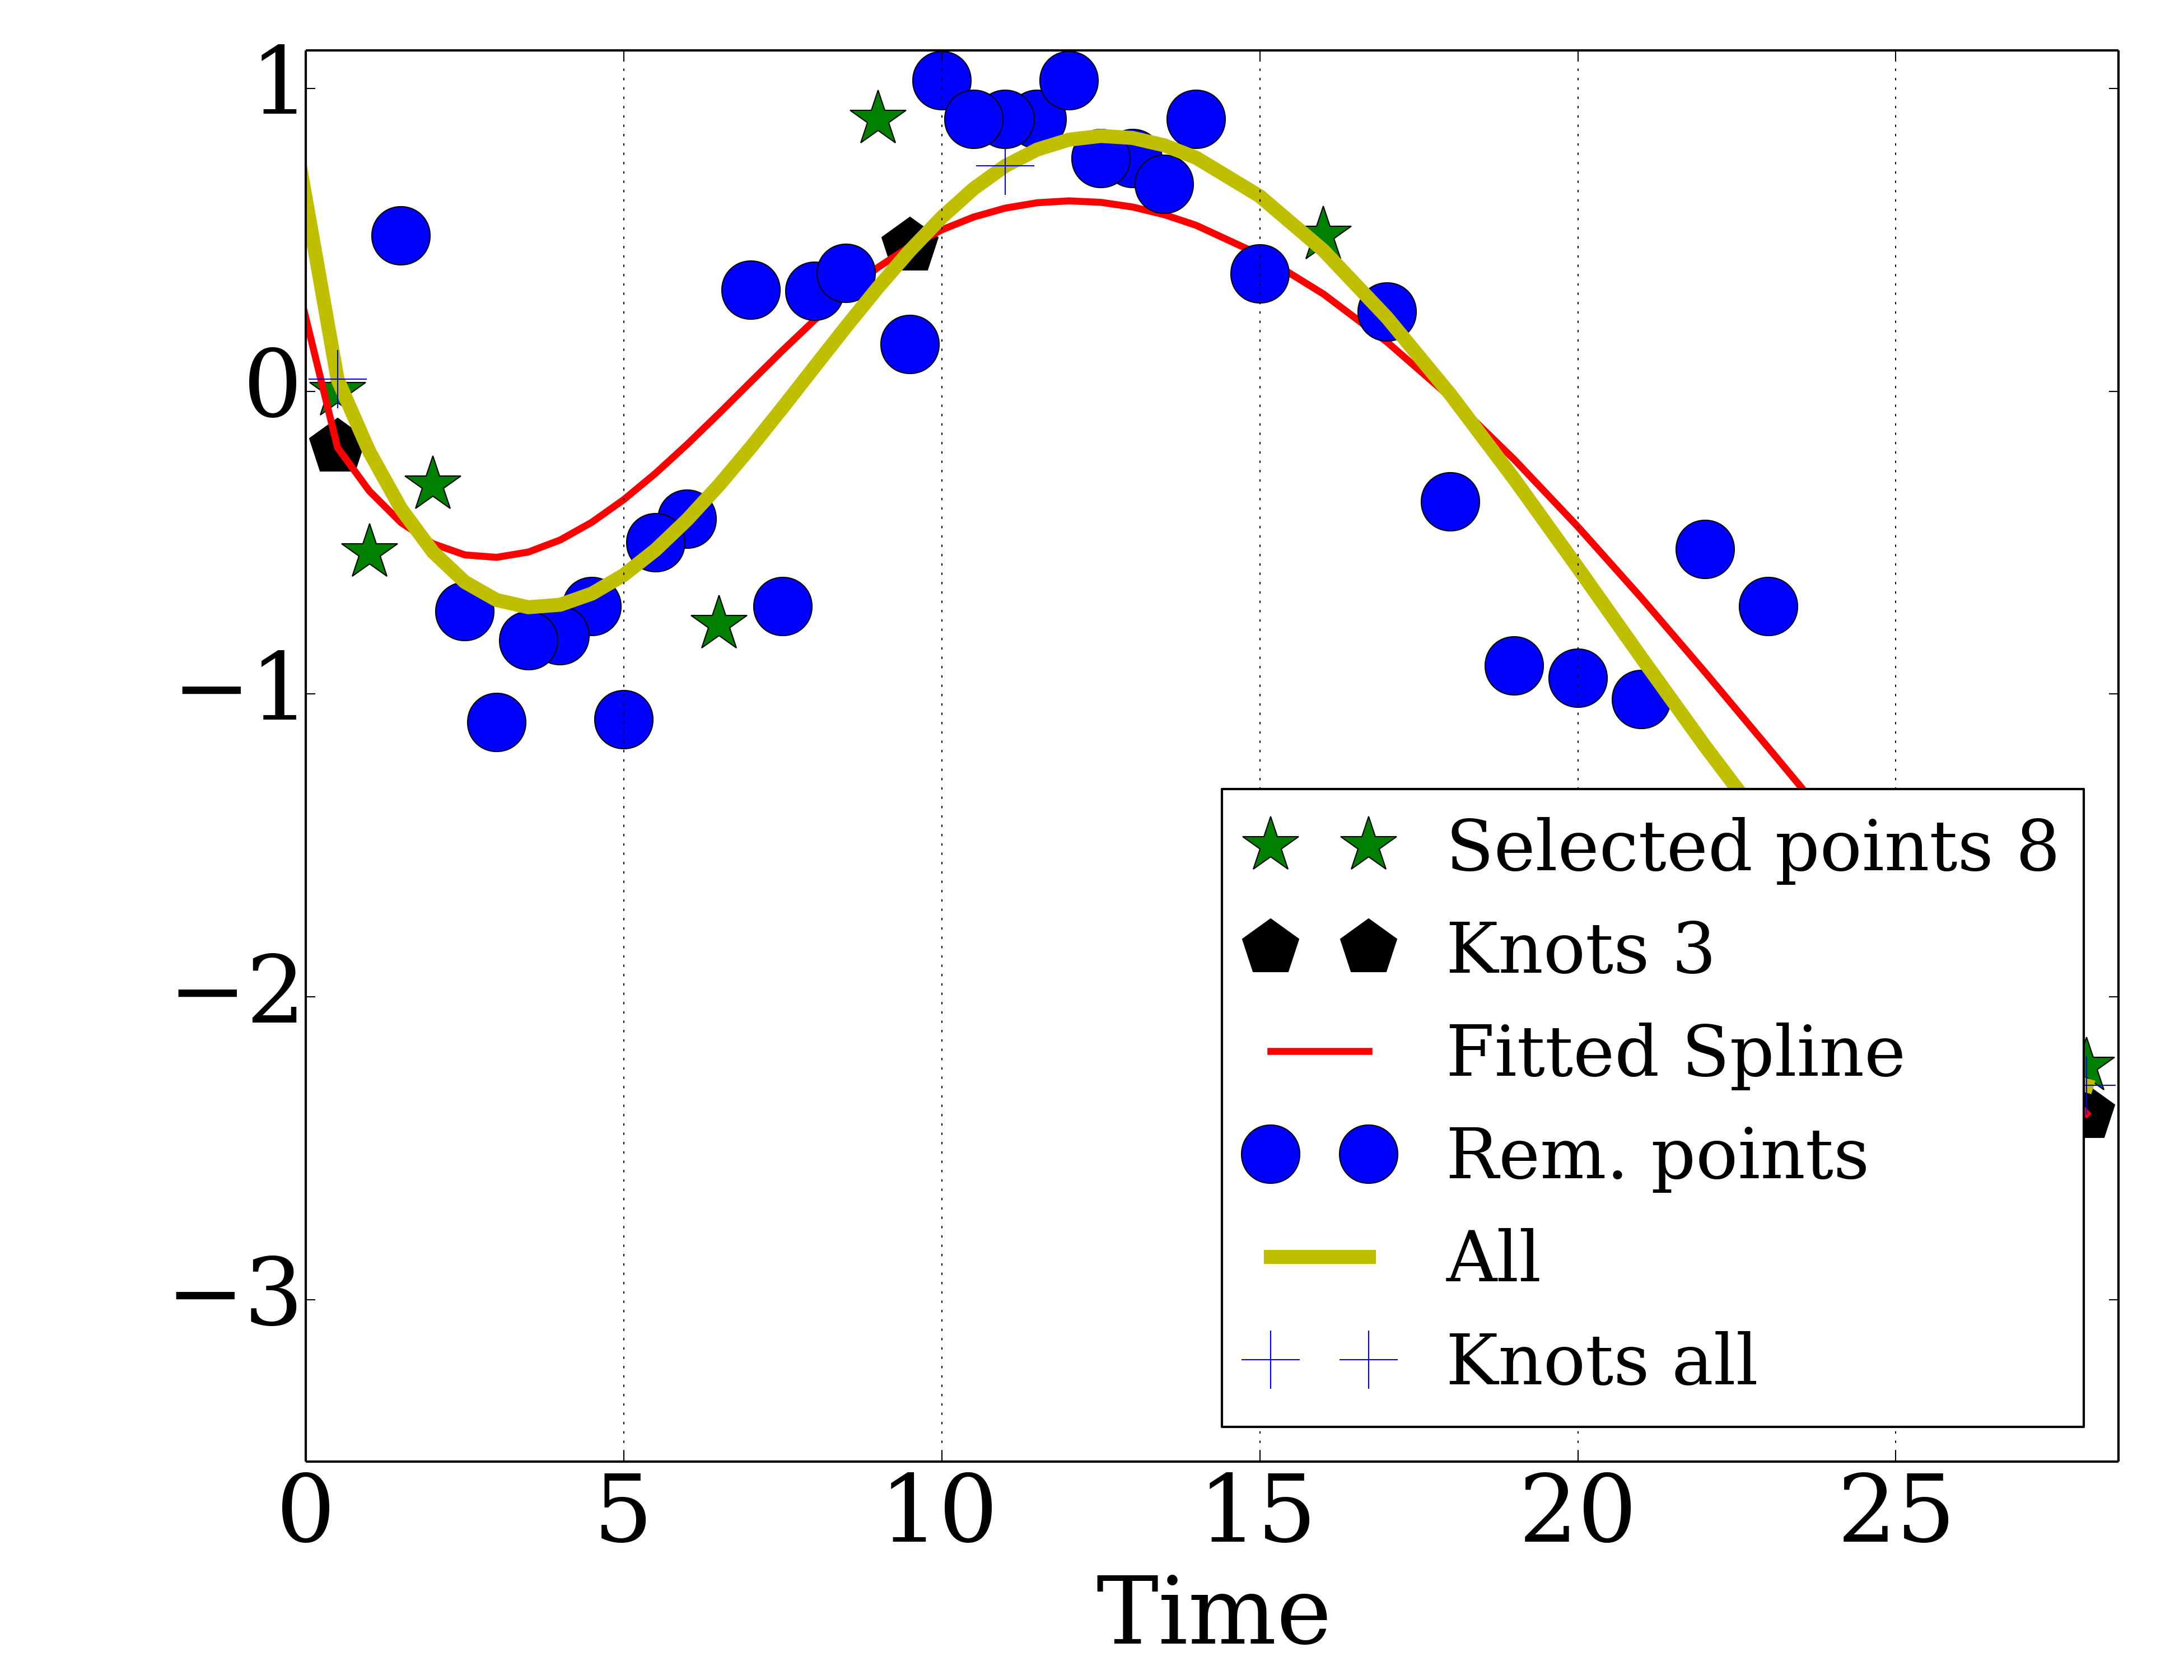
\includegraphics[scale=0.12]{{plots/newdata/splineplots8/Eln_8_all}.png}}
\hfill
\subfloat[INMT]{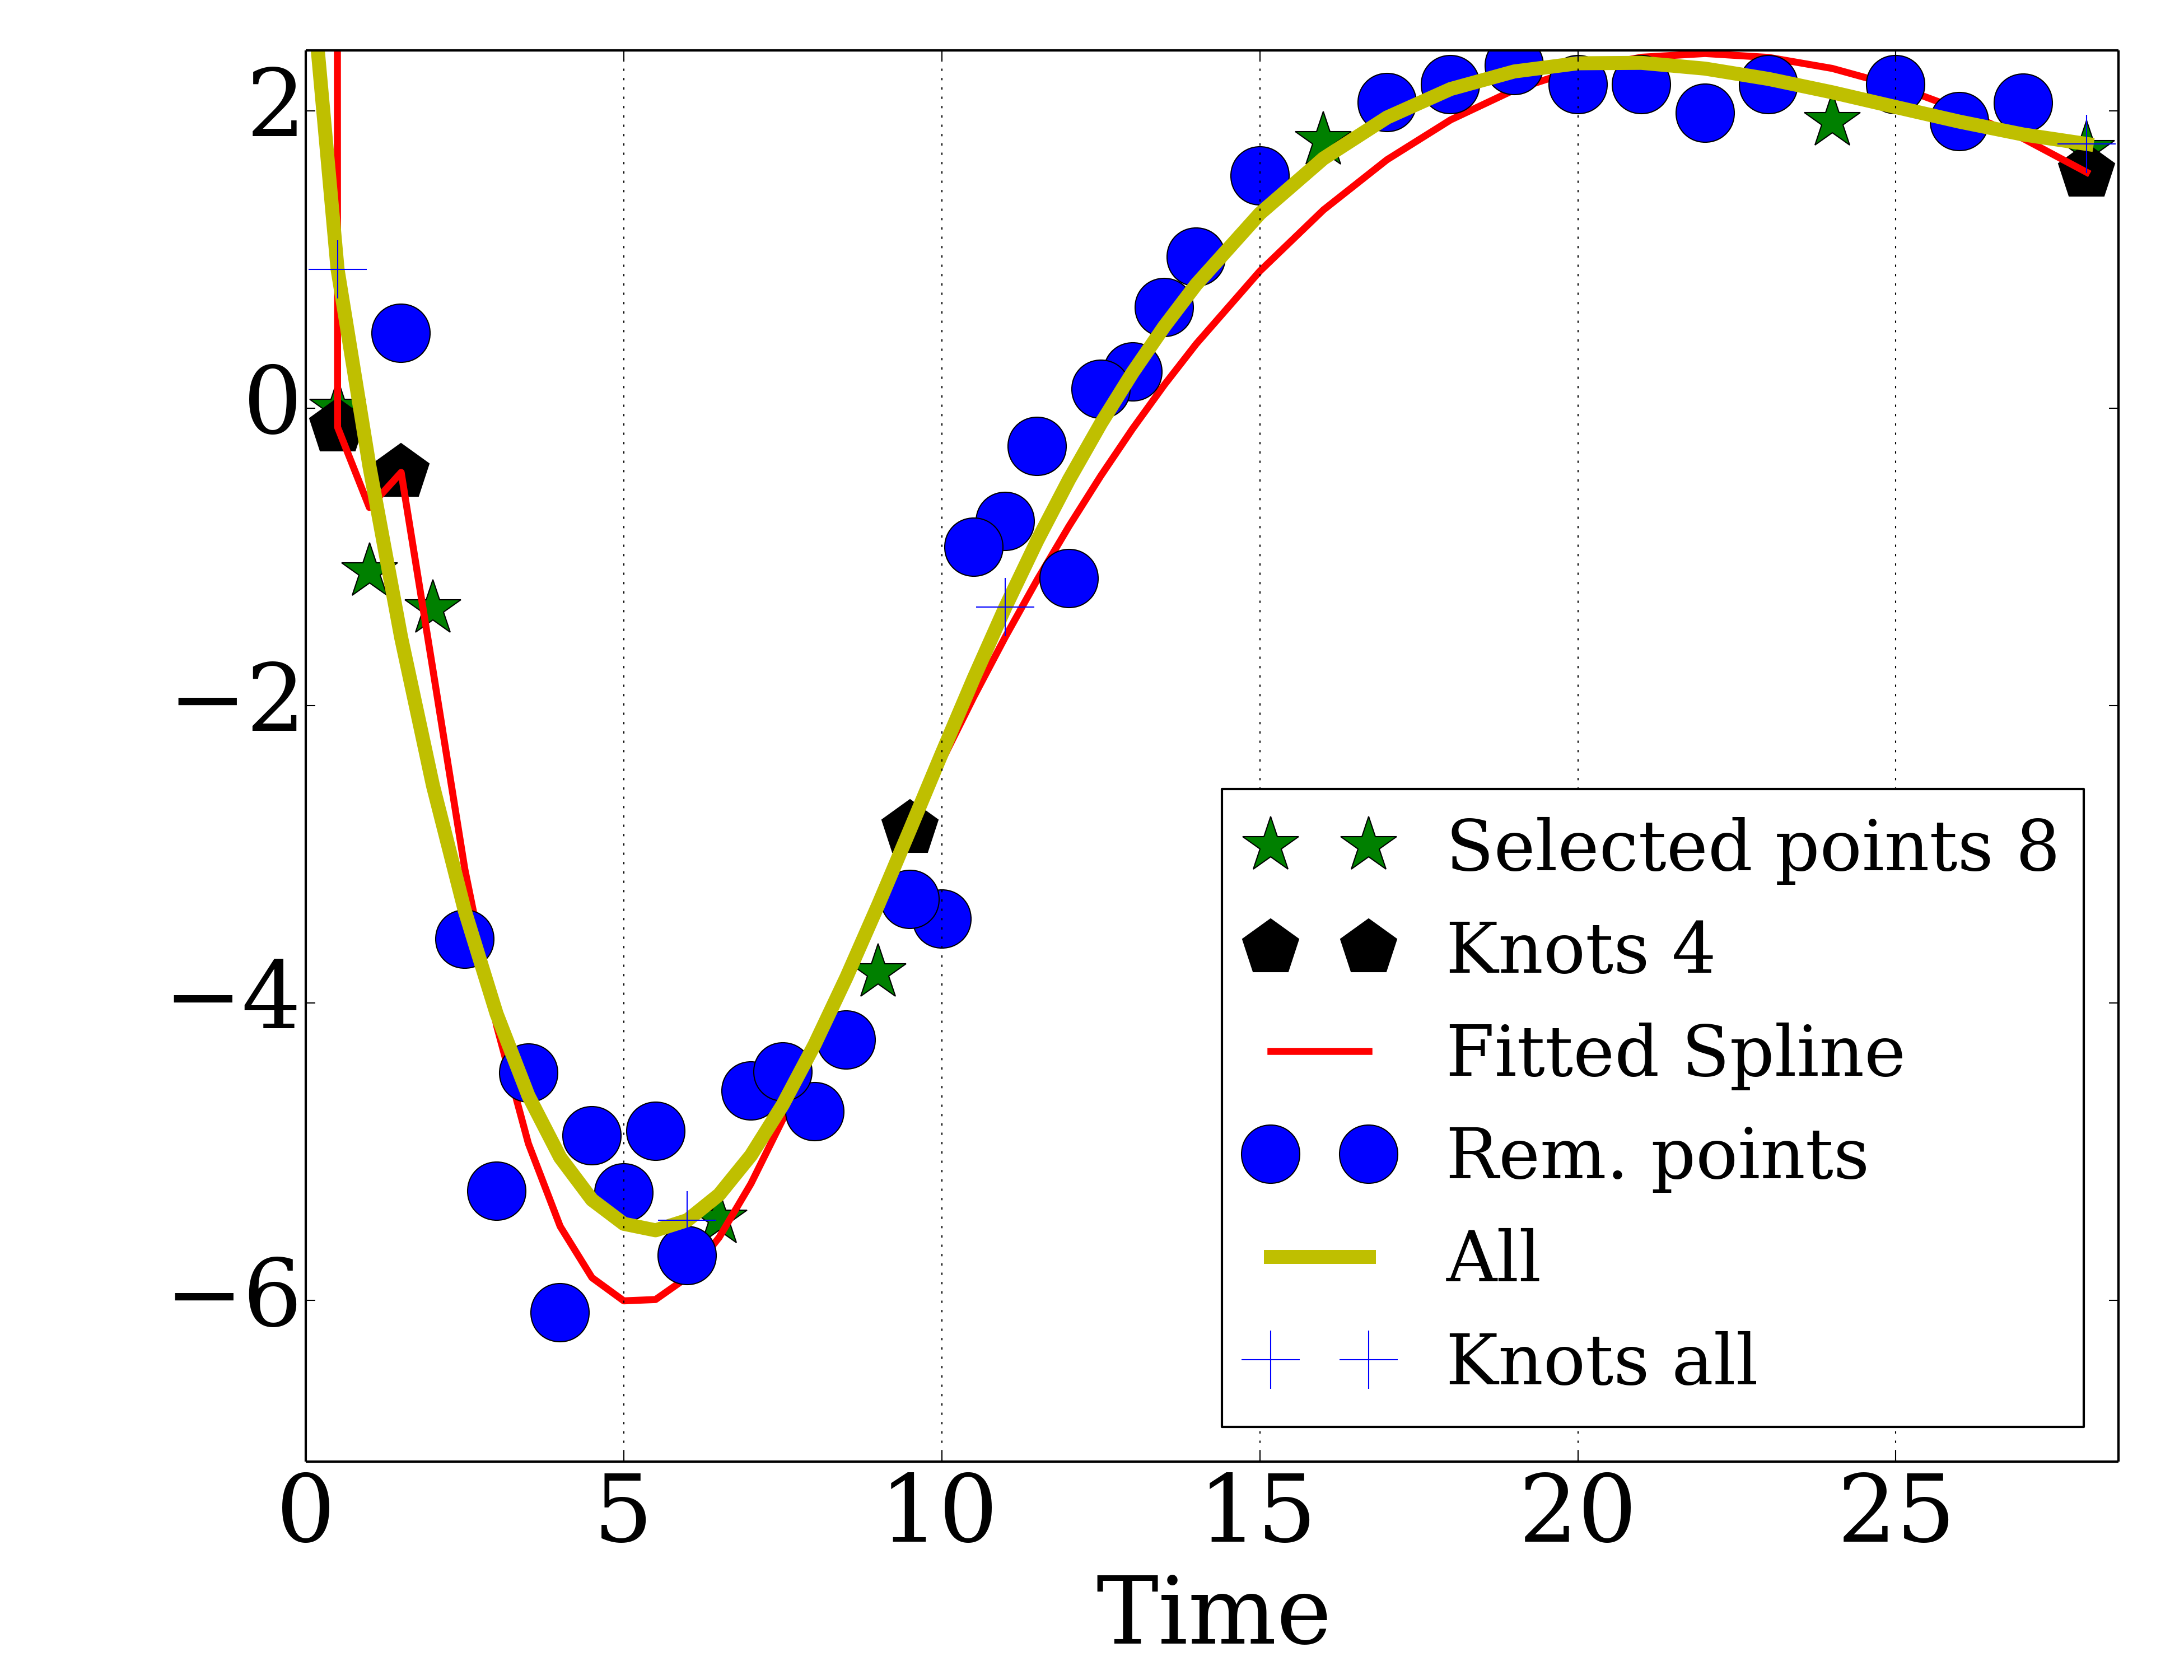
\includegraphics[scale=0.12]{{plots/newdata/splineplots8/INMT_8_all}.png}}
\hfill
\end{minipage}
\caption{Reconstructed expression profiles by $8$ points over genes a) PDGFRA, b) ELN, c) INMT}
\label{fig:sup4}
\end{figure}

\begin{figure}
\begin{minipage}{1.0\textwidth}
\subfloat[PDGFRA]{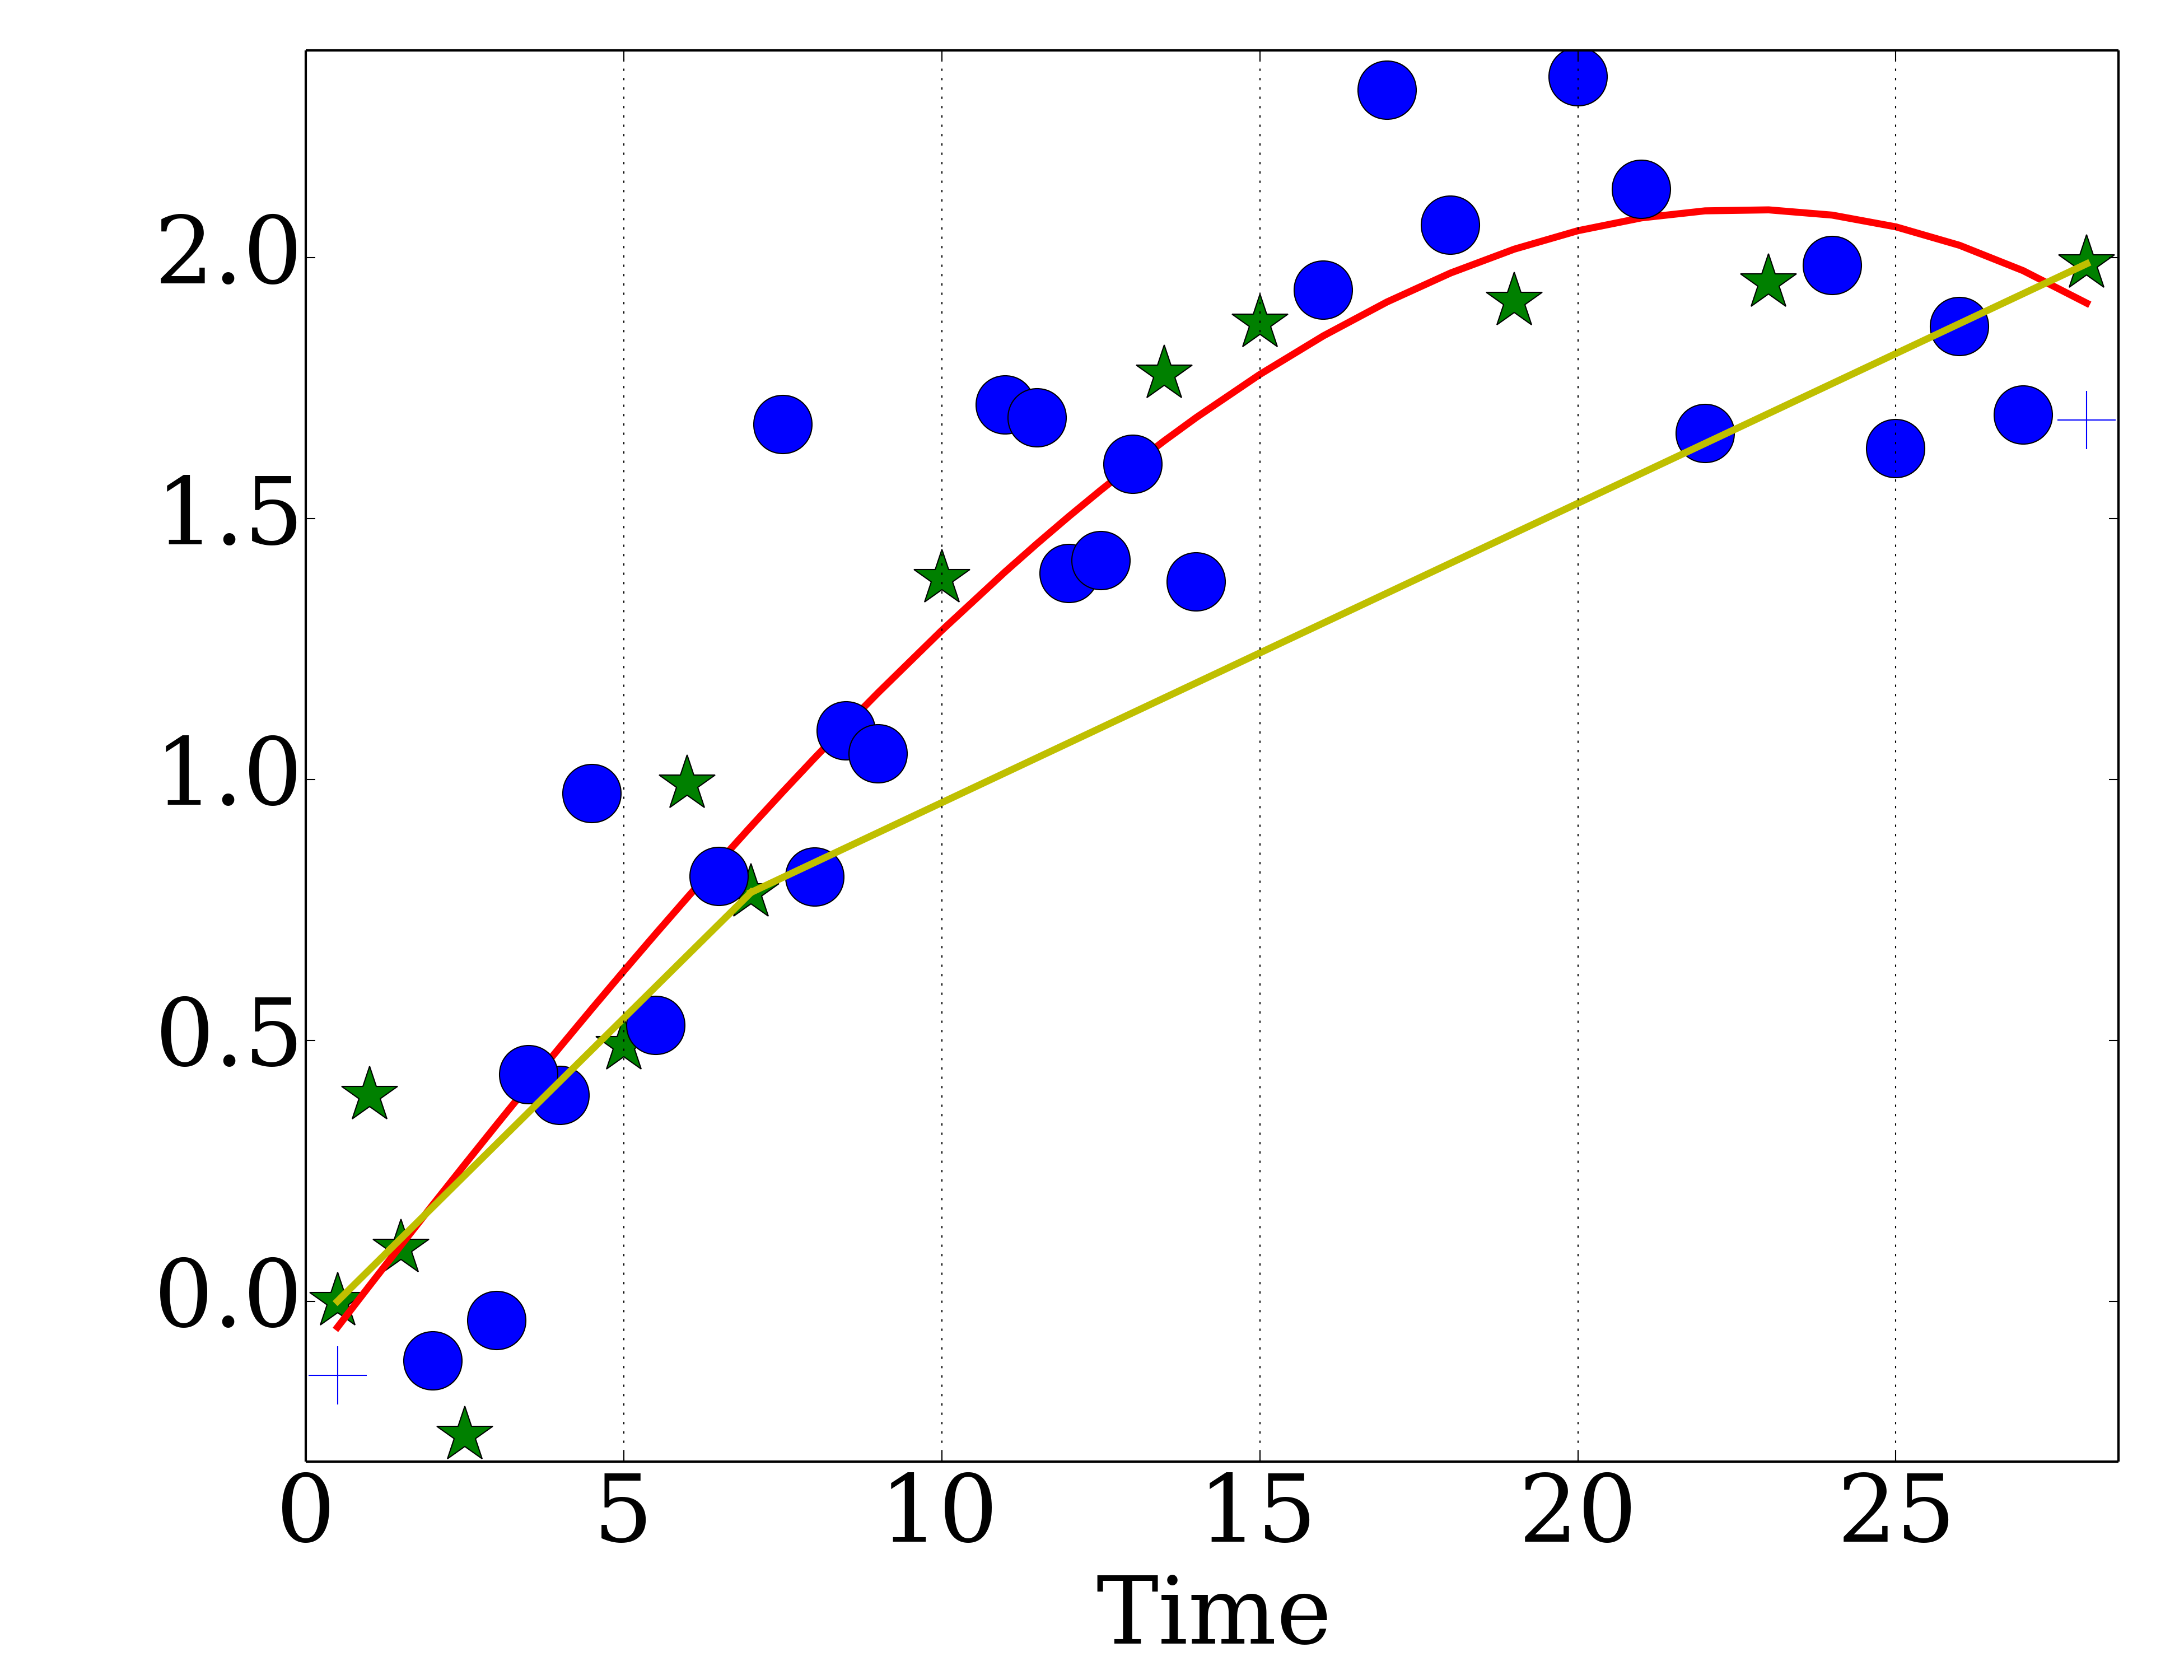
\includegraphics[scale=0.12]{{plots/newdata/splineAndLinear/17_PDGFRA_13_all}.png}}
\hfill
\subfloat[ELN]{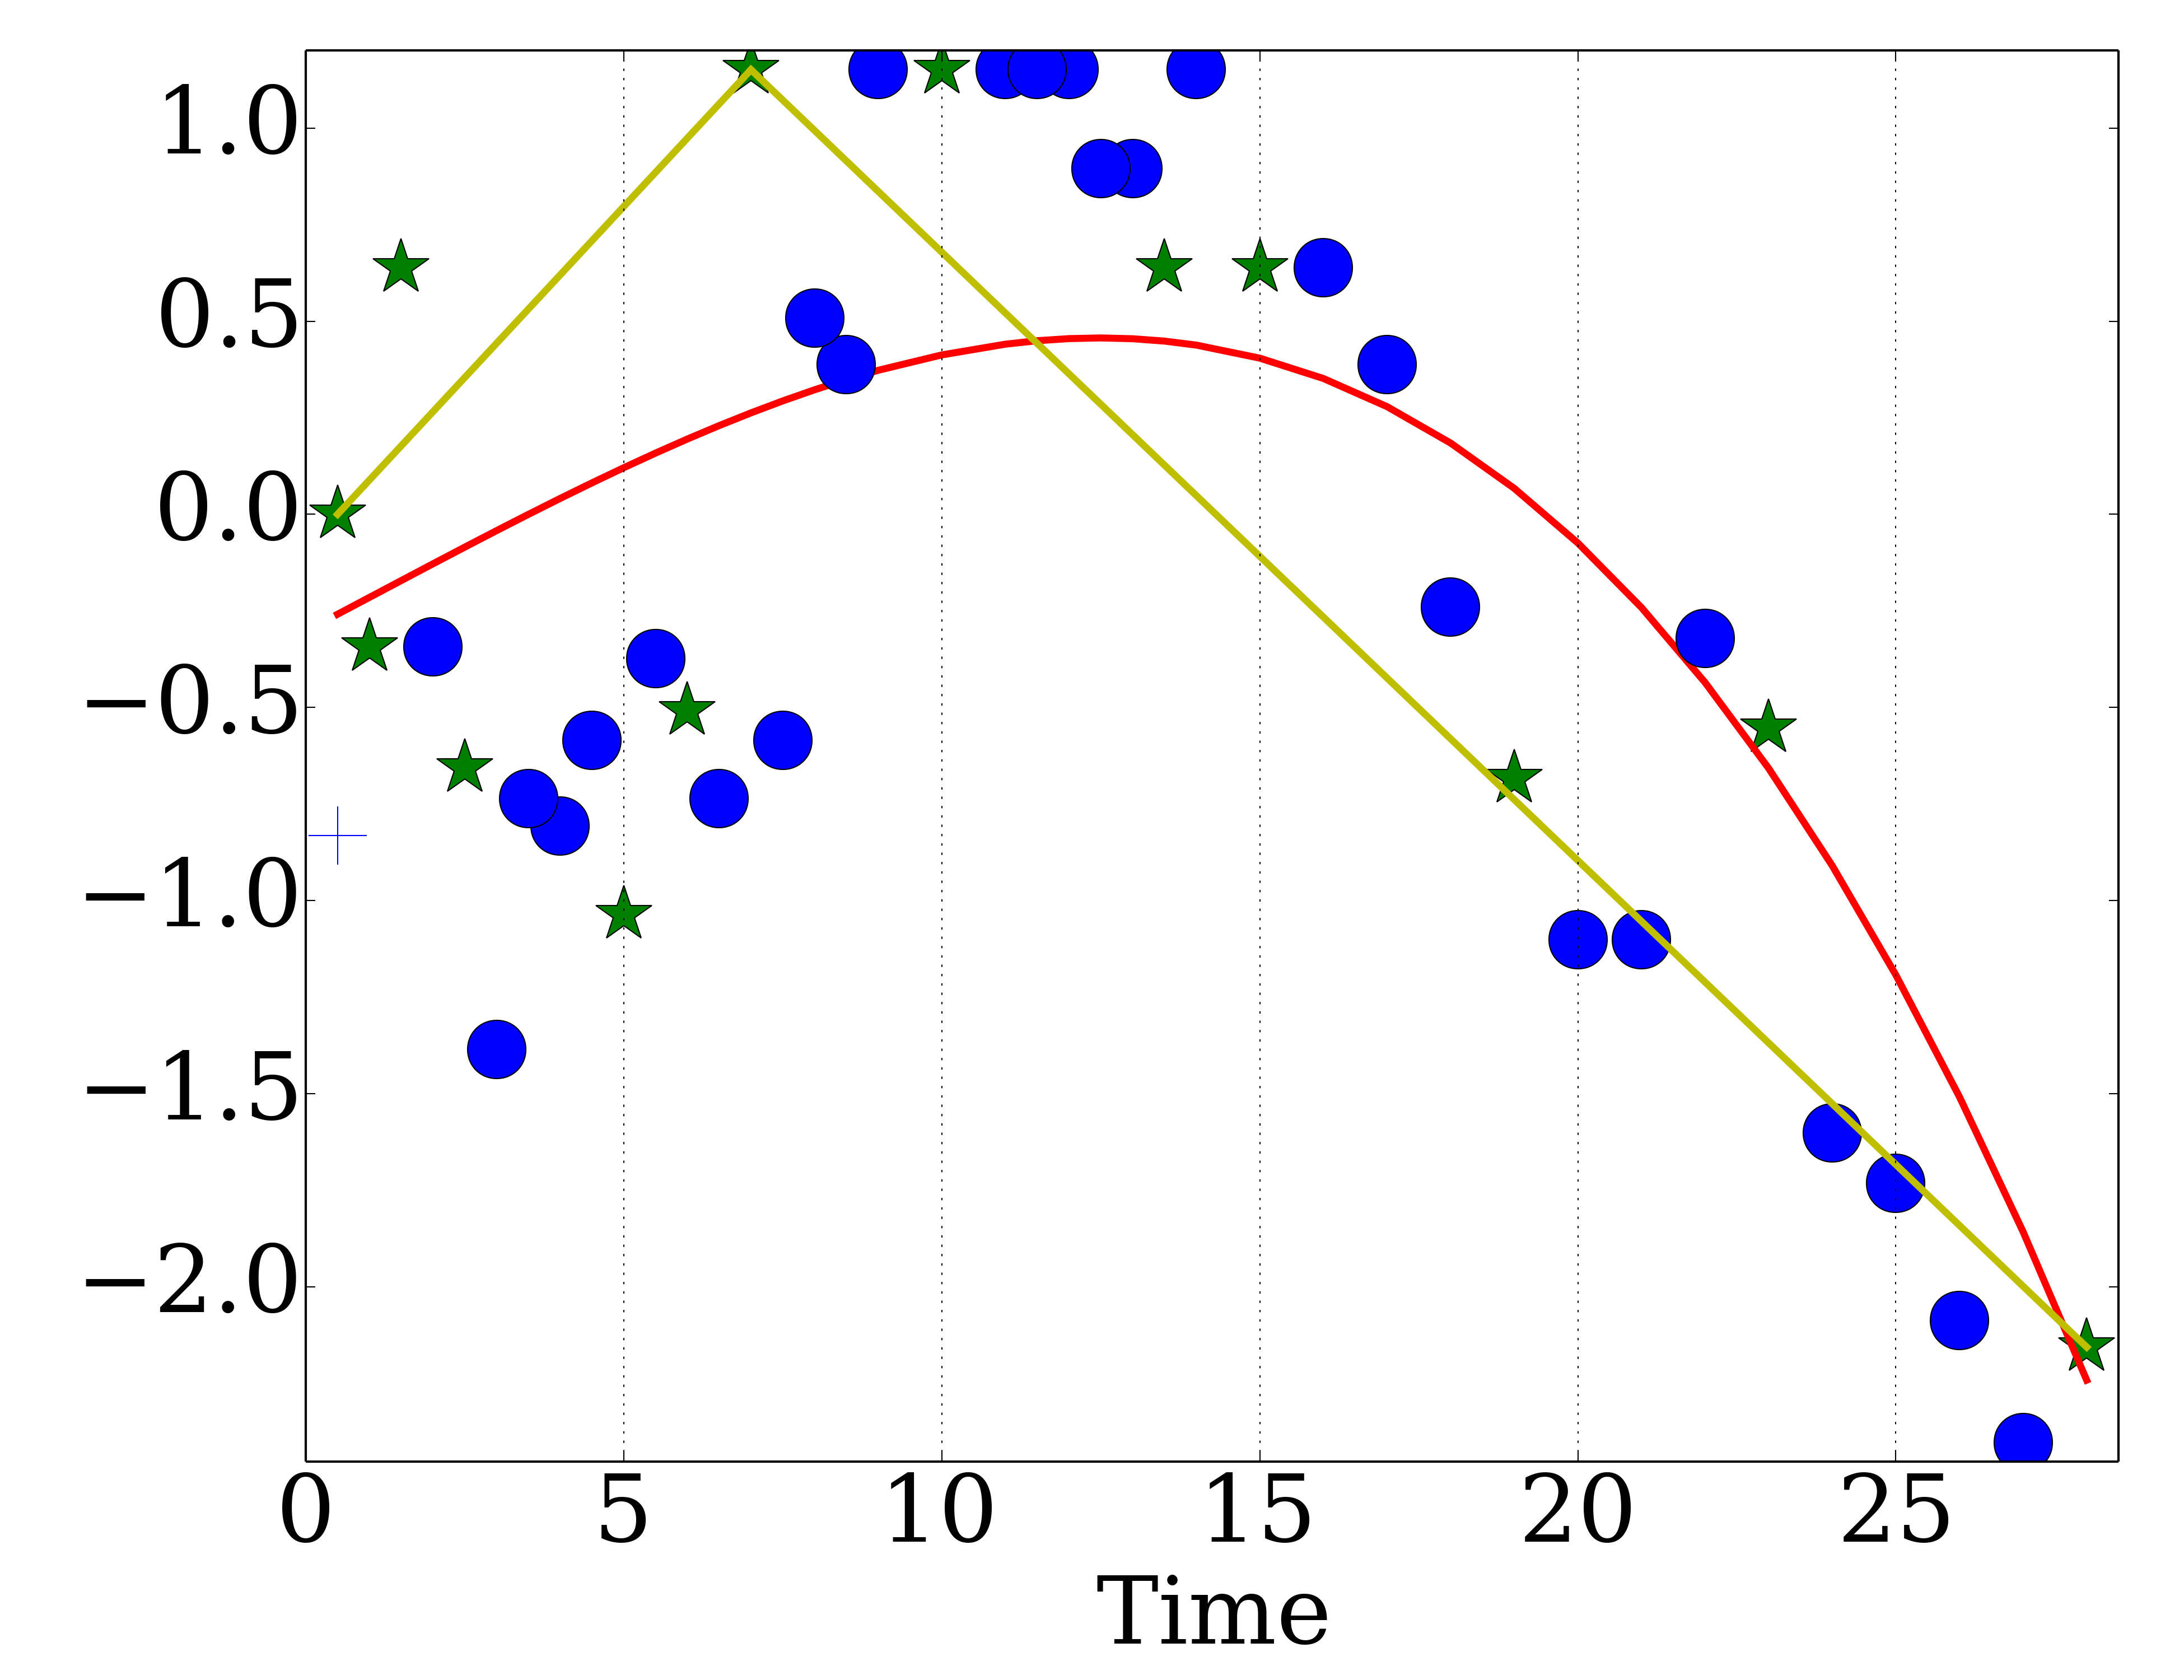
\includegraphics[scale=0.12]{{plots/newdata/splineAndLinear/14_Eln_13_all}.png}}
\hfill
\subfloat[LRAT]{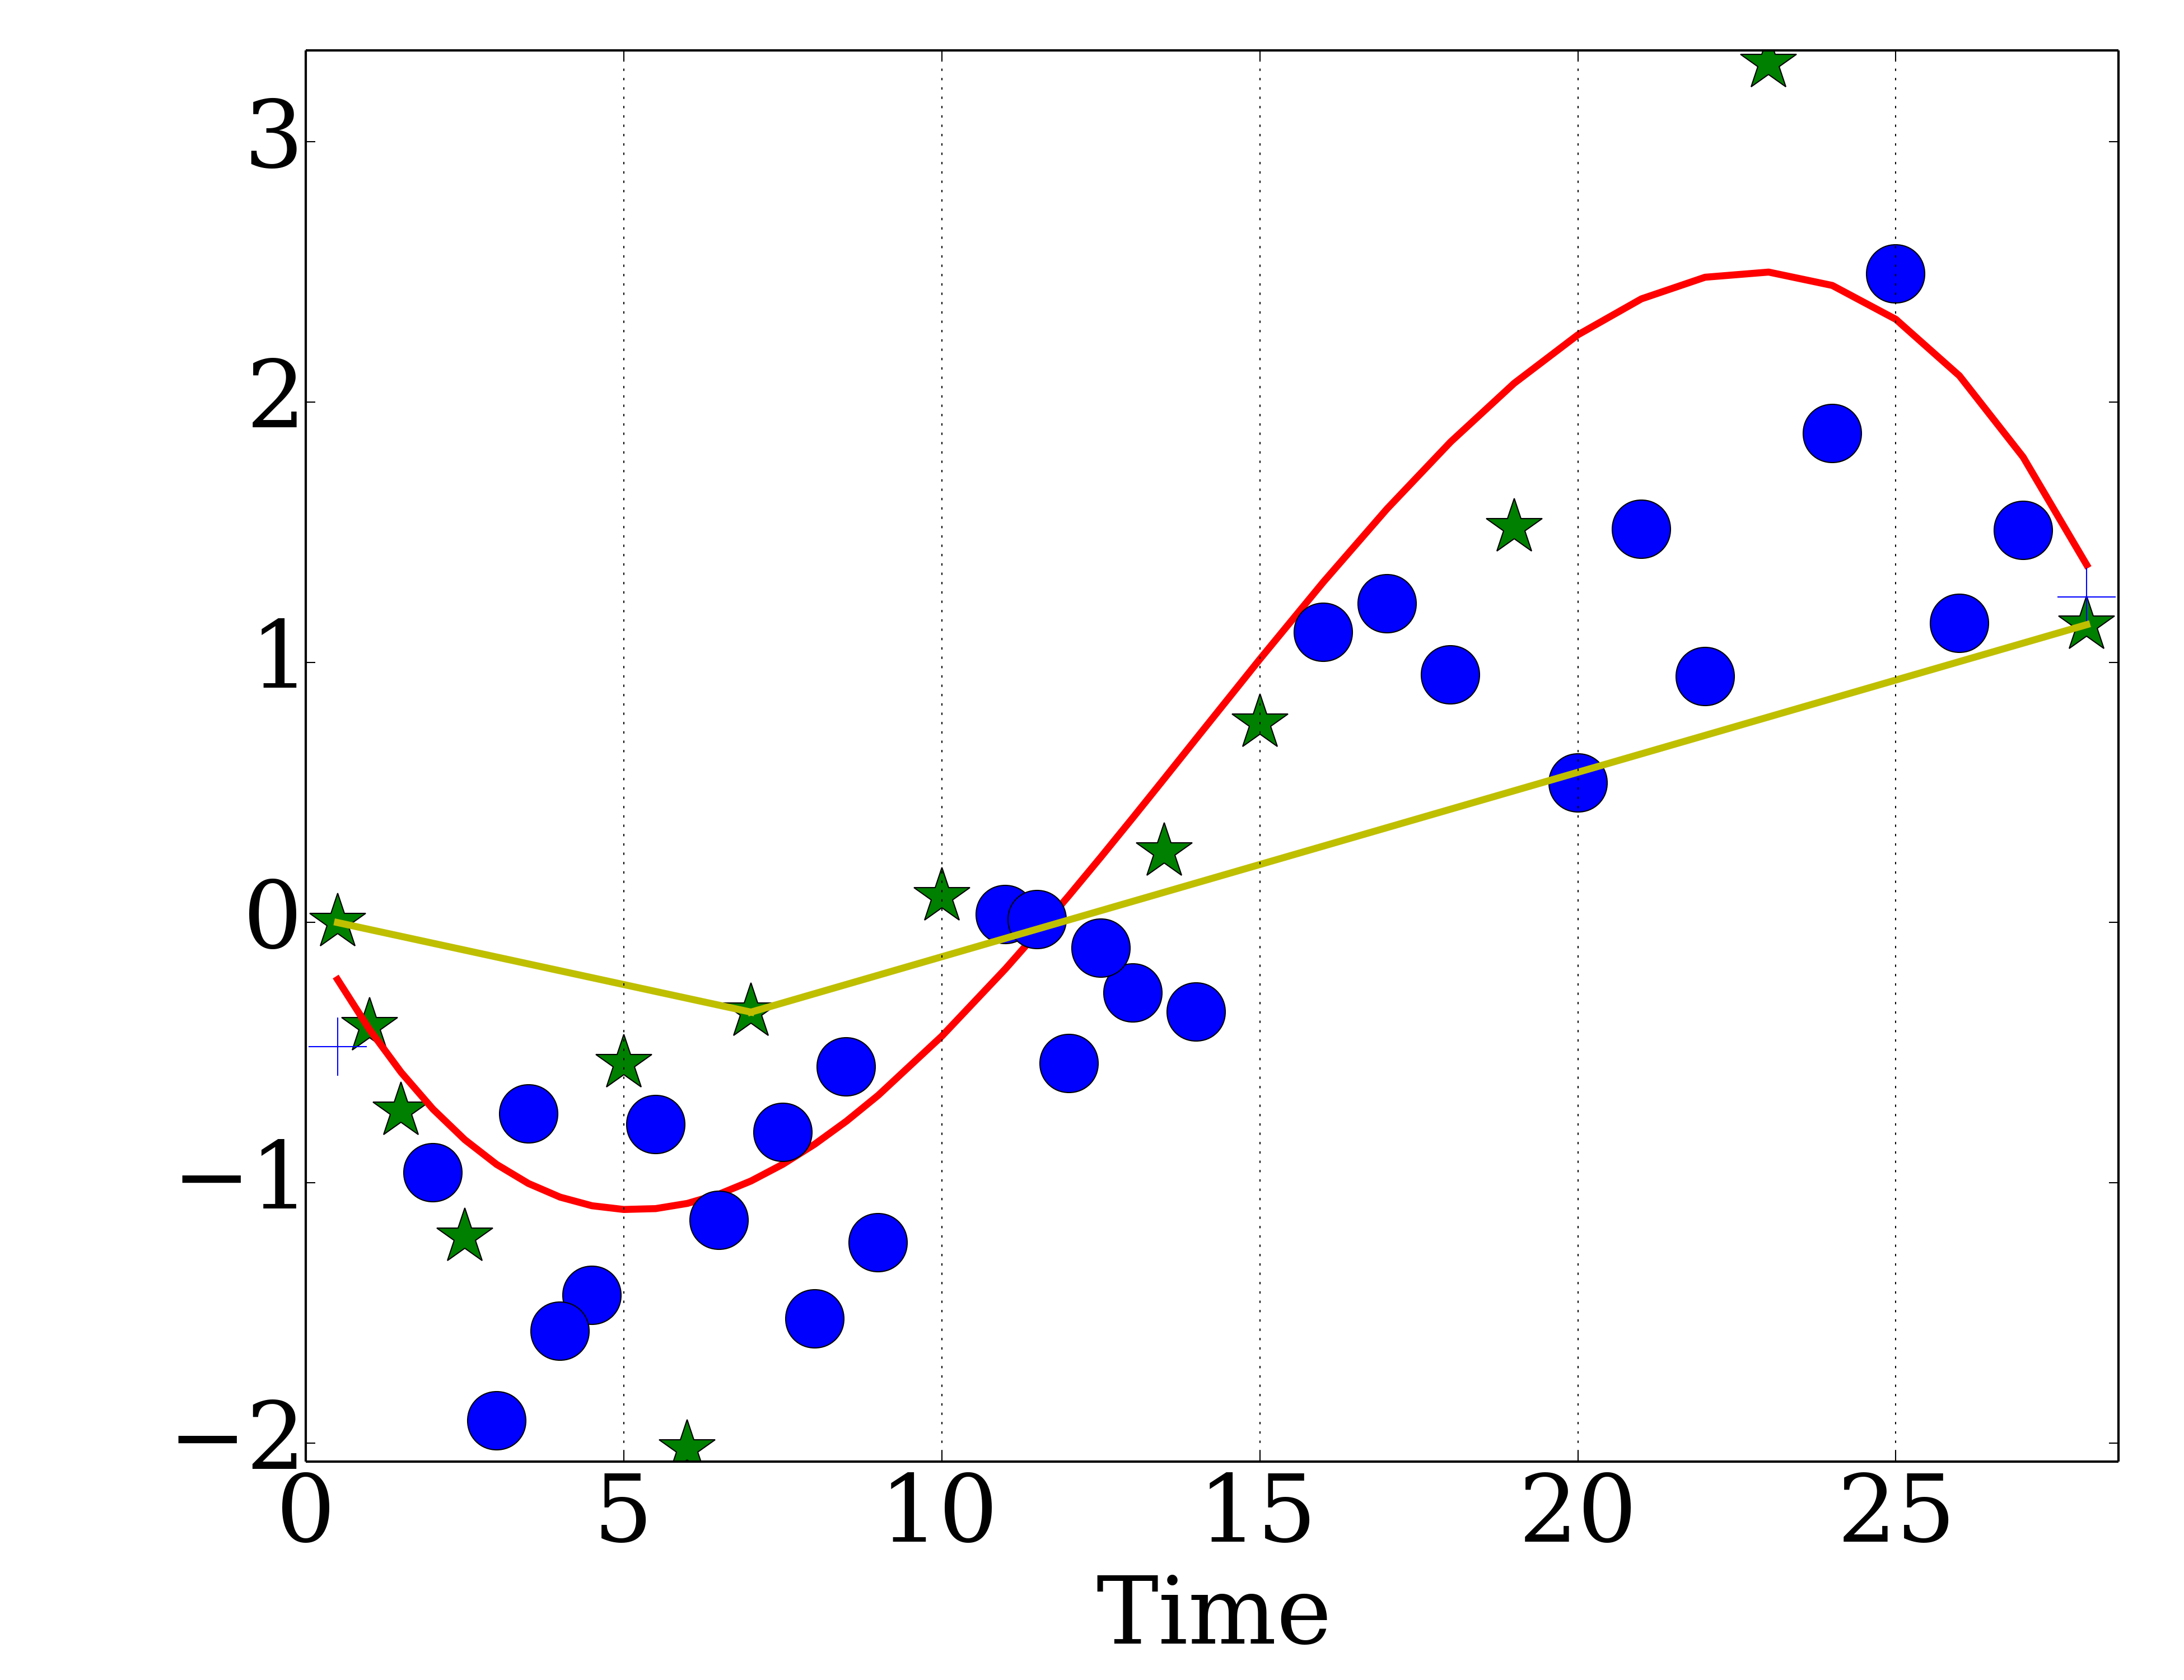
\includegraphics[scale=0.12]{{plots/newdata/splineAndLinear/1_LRAT_13_all}.png}}
\hfill
\end{minipage}
\caption{Comparison of \Tempselect and piecewise linear fitting over
  genes a) PDGFRA, b) ELN, c) LRAT}
\label{fig:sup5}
\end{figure}

\begin{figure}
\begin{minipage}{1.0\textwidth}
\subfloat[6 stable clusters]{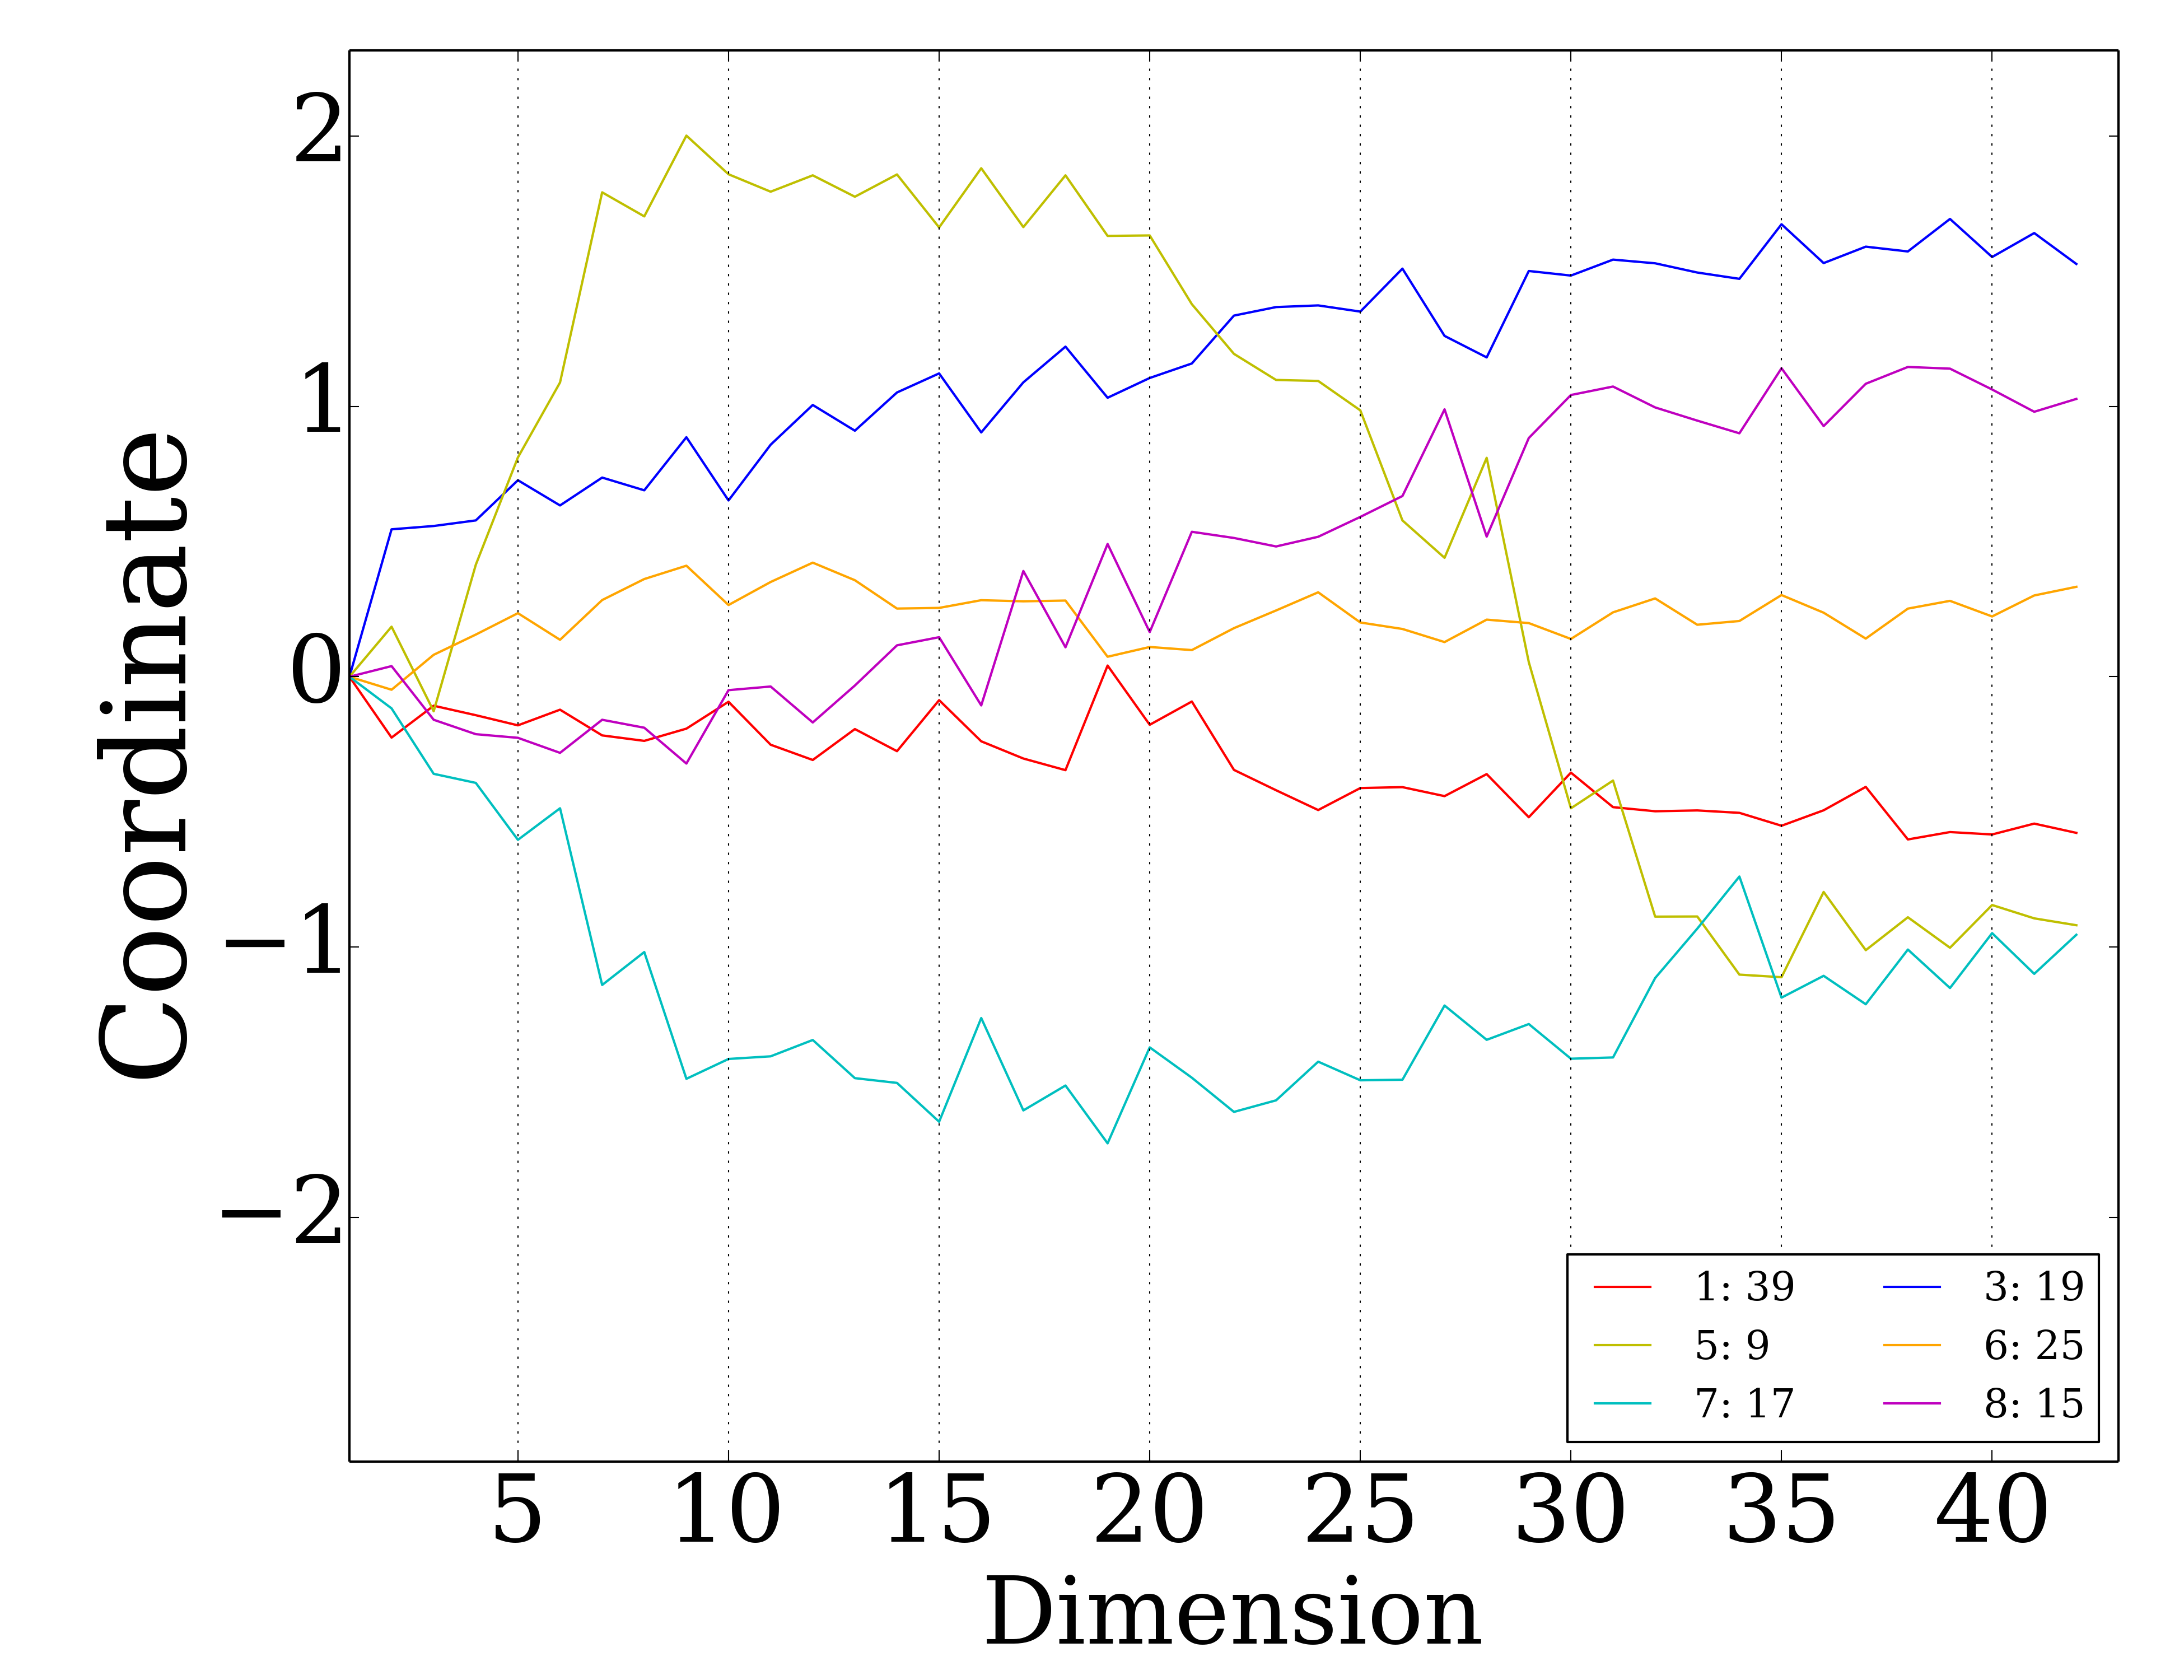
\includegraphics[scale=0.15]{{plots/newdata/centplotlimit}.png}}
\hfill
\subfloat[Centroids]{\includegraphics[scale=0.15]{{plots/newdata/centplot}.png}}
\end{minipage}
\caption{}
\label{fig:sup6}
\end{figure}

\begin{table}[ht]
\centering
\begin{tabular}{|c|c|c|c|c|}
\hline
Gene & Number of loci  & & Gene & Number of loci  \\
\hline
Cdh11 & 14 & & Zfp536 & 16 \\
\hline
Src & 11 & & Igfbp3 & 34 \\
\hline
Sox9 & 16 & & Wif1 & 21 \\
\hline
Dnmt3a & 41 & & Vegfa & 20 \\
\hline
Eln & 20 & & Tnc & 4 \\
\hline
Foxf2 & 41 & & Lox & 17 \\
\hline
Akt1 & 11 & & &  \\
\hline
\end{tabular}
\caption{Summary of methylation dataset}
\label{tab:sup1}
\end{table}

\begin{table}
\centering
\begin{tabular}{|c|c|c|c|c|}
\hline
Gene & $r$  & & Gene & $r$ \\
\hline
Cdh11 & $0.60$ & & Lox & $0.88$ \\
\hline
Src & $0.77$ & & Igfbp3 & $0.55$ \\
\hline
Sox9 & $0.45$ & & Wif1 & $0.54$ \\
\hline
Dnmt3a & $0.82$ & & Vegfa & $0.60$ \\
\hline
Eln & $0.72$ & & Tnc & $-0.36$ \\
\hline
Foxf2 & $0.62$ & & & \\
\hline
Akt1 & $0.13$ & & &  \\
\hline
\end{tabular}
\caption{Pearson correlation $r$  between expression and
  methylation datasets over $8$ time points for each gene.}
\label{tab:sup2}
\end{table}


\end{document}
